% Document class
\documentclass[8pt,a4paper]{article}

% Packages
\usepackage[utf8]{inputenc}
\usepackage[top=1.5cm, bottom=1.5cm, left=1cm, right=1cm]{geometry}
\usepackage{amsmath}
\usepackage{amssymb}
\usepackage{graphicx}
\usepackage{float}
\usepackage{adjustbox}
\usepackage{hyperref}

% Hyperref setup
\hypersetup{
    colorlinks=true,
    linkcolor=blue,
    urlcolor=blue
}

\title{Homework 1 - VLSI II}
\author{Demian Marin - dm6430}
\date{\today}




\begin{document}
\maketitle	

\section*{Problem 1}

\begin{figure}[h]
    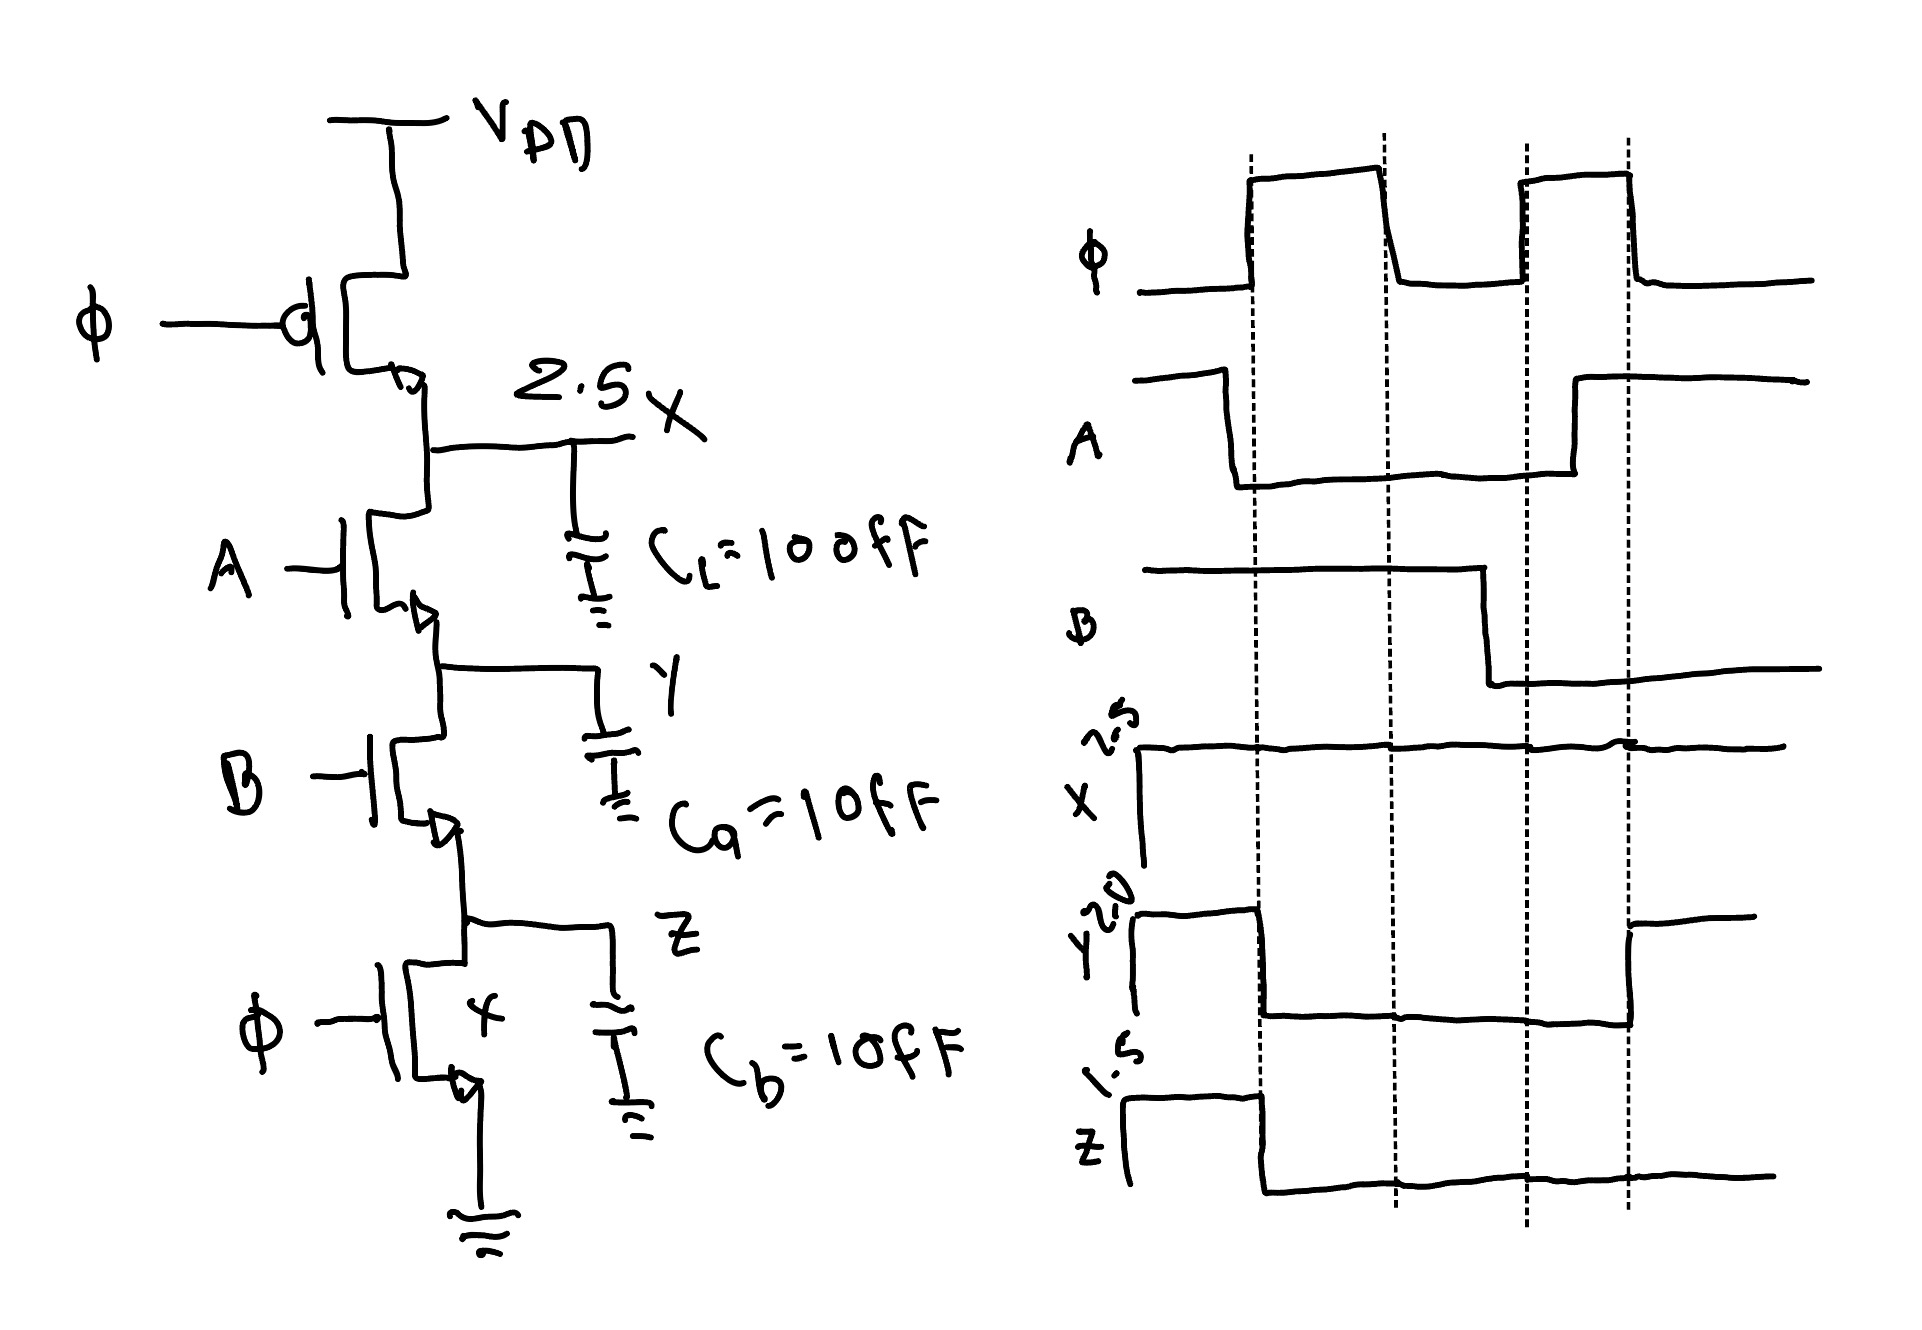
\includegraphics[width=0.45\textwidth]{Images/sketch_p1.jpg}
    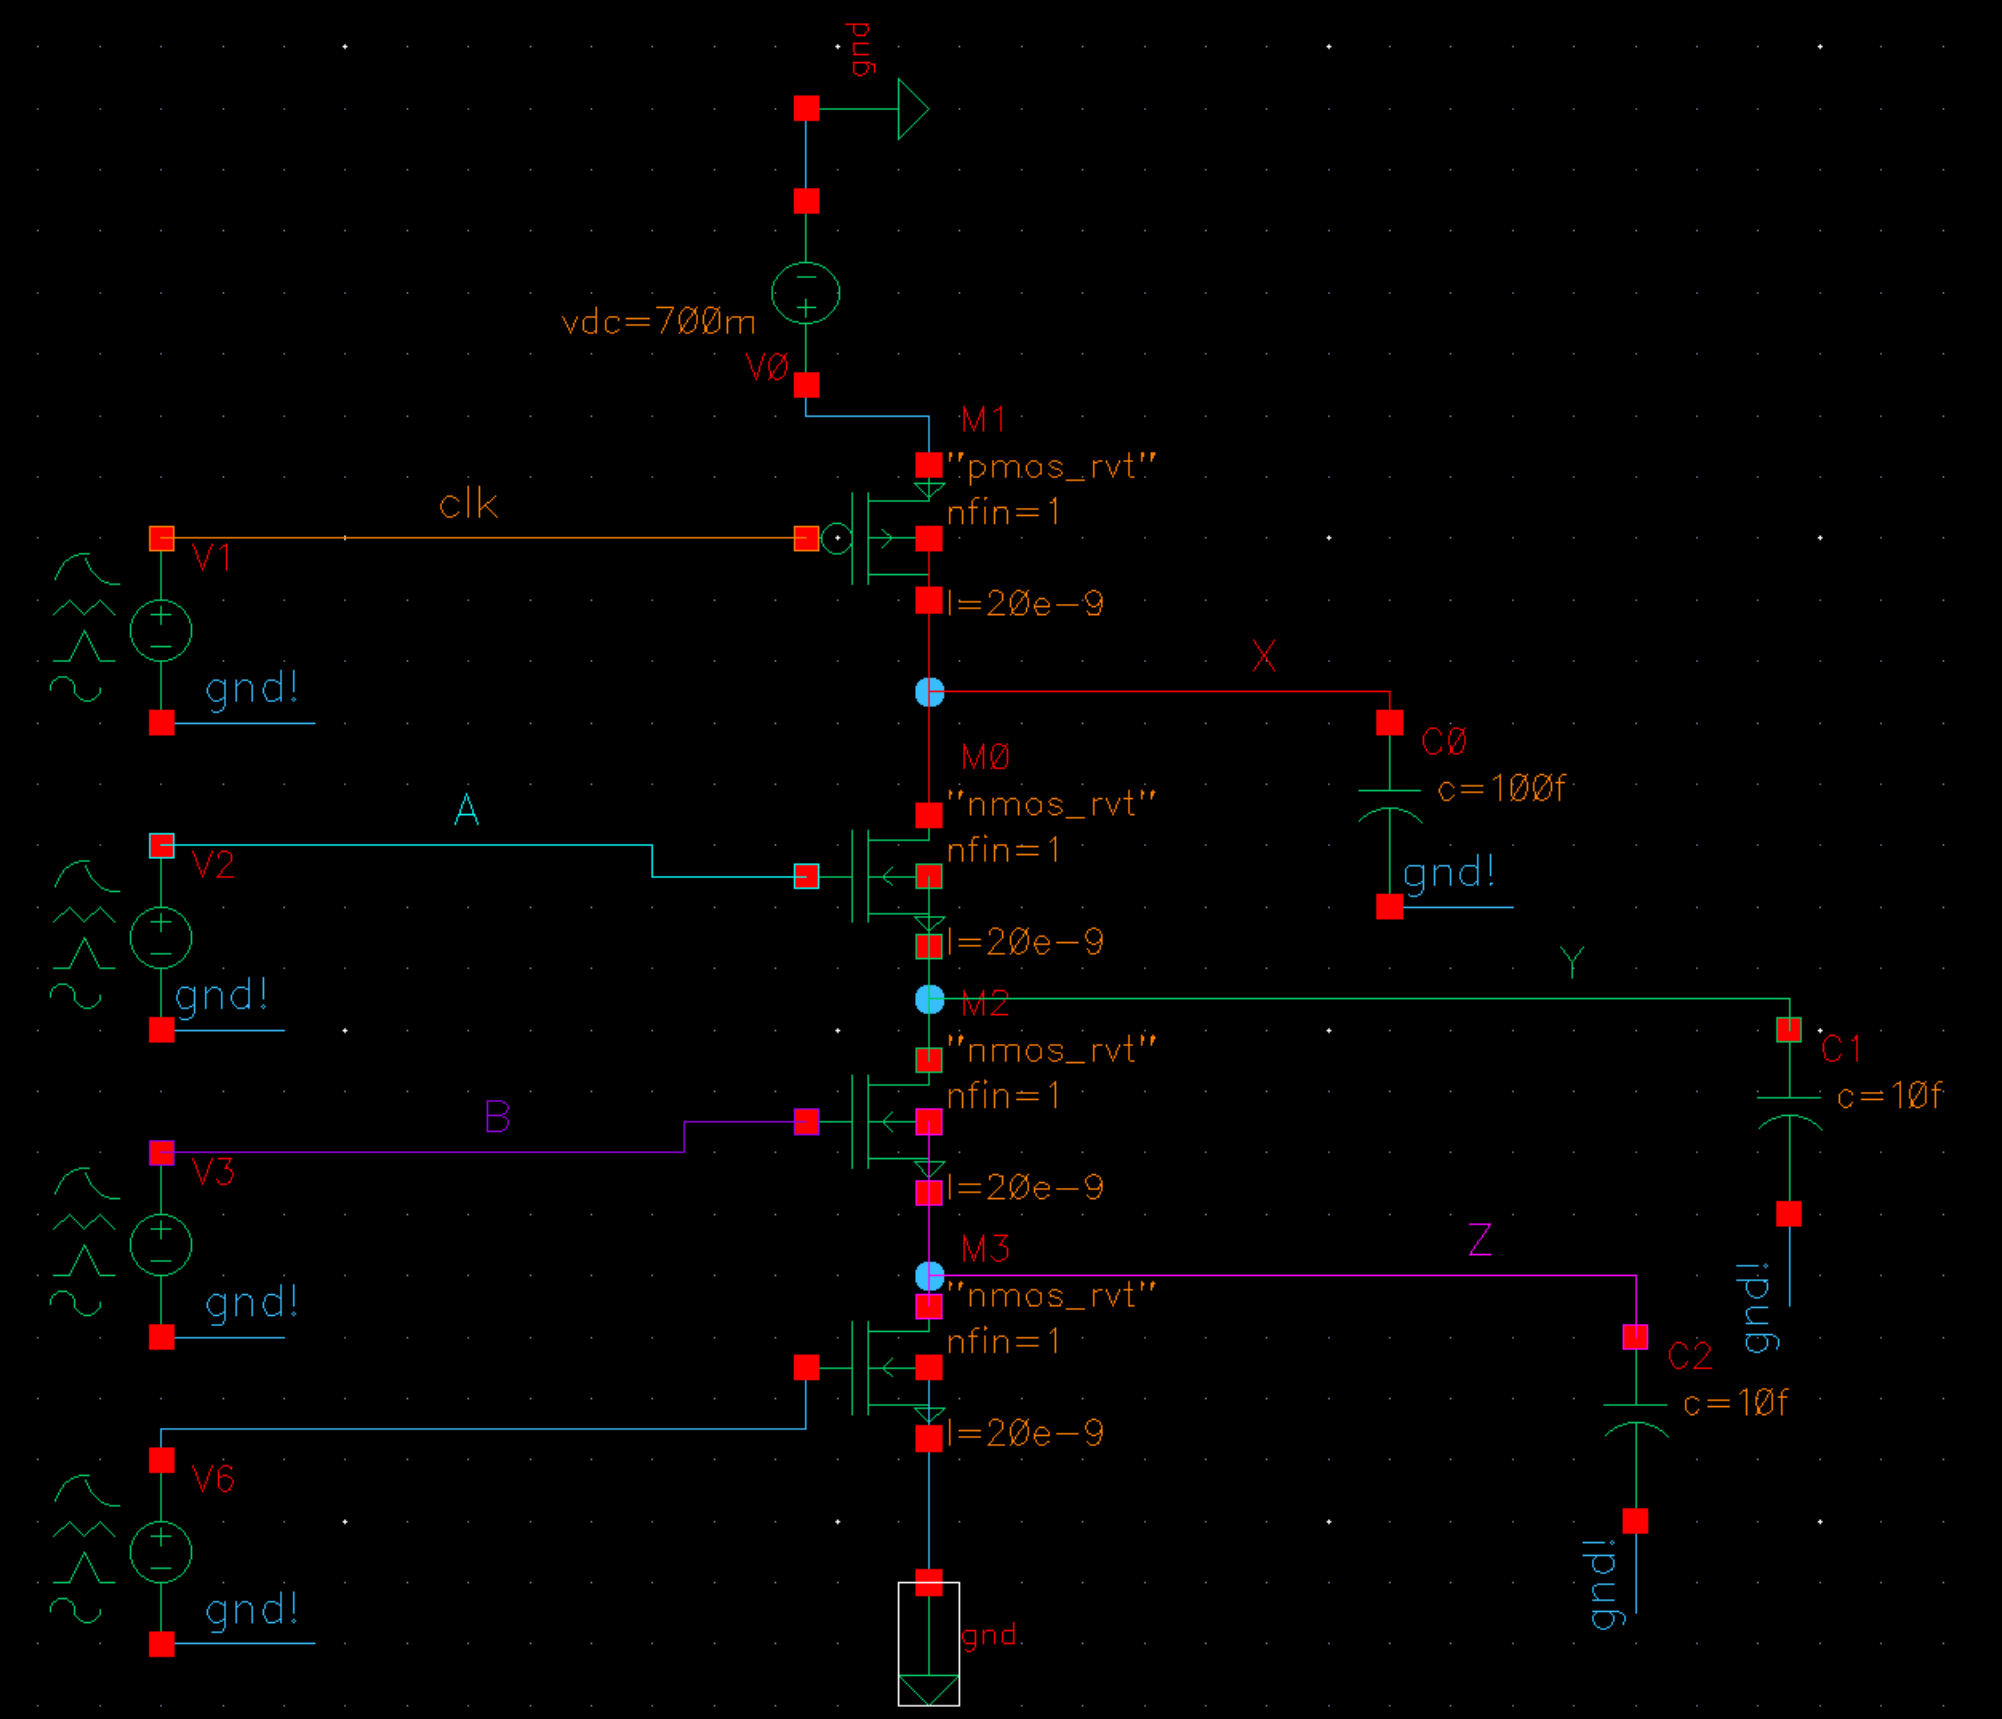
\includegraphics[width=0.65\textwidth]{Images/sch_p1.png}
    \caption{Problem 1. Wave sketch (left) and Schematic (right) problem 1}
    \label{fig:sketch_sch_problem1}
\end{figure}

\begin{figure}[h]
    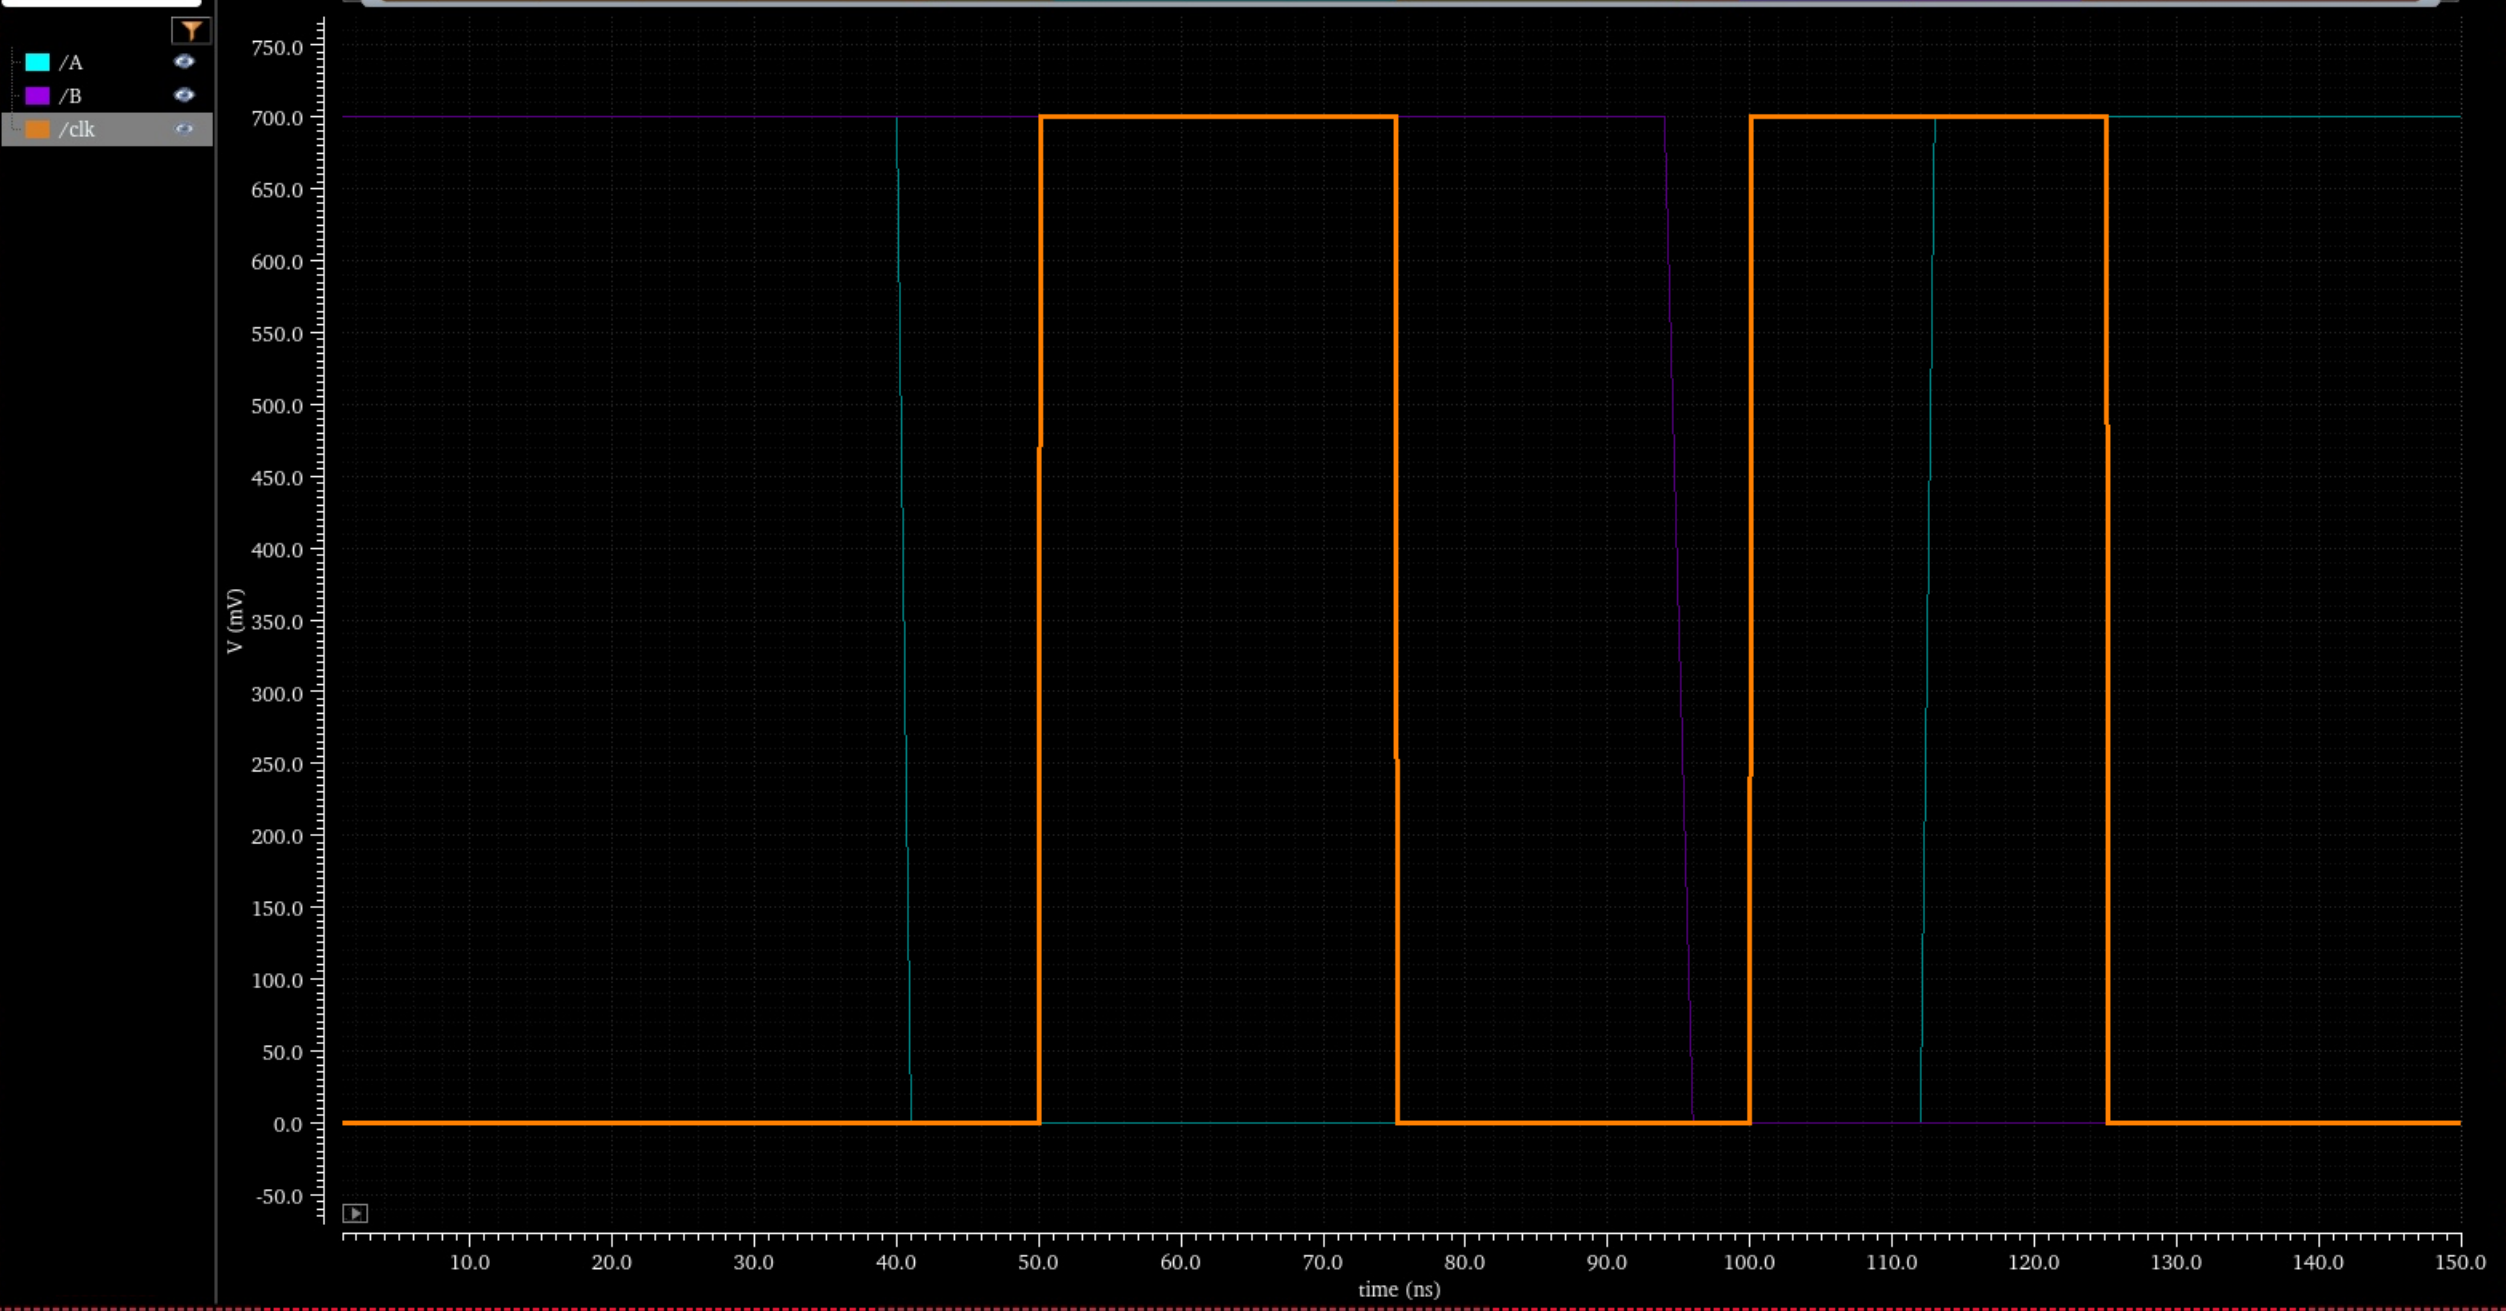
\includegraphics[width=0.50\textwidth]{Images/input_p1.png}
    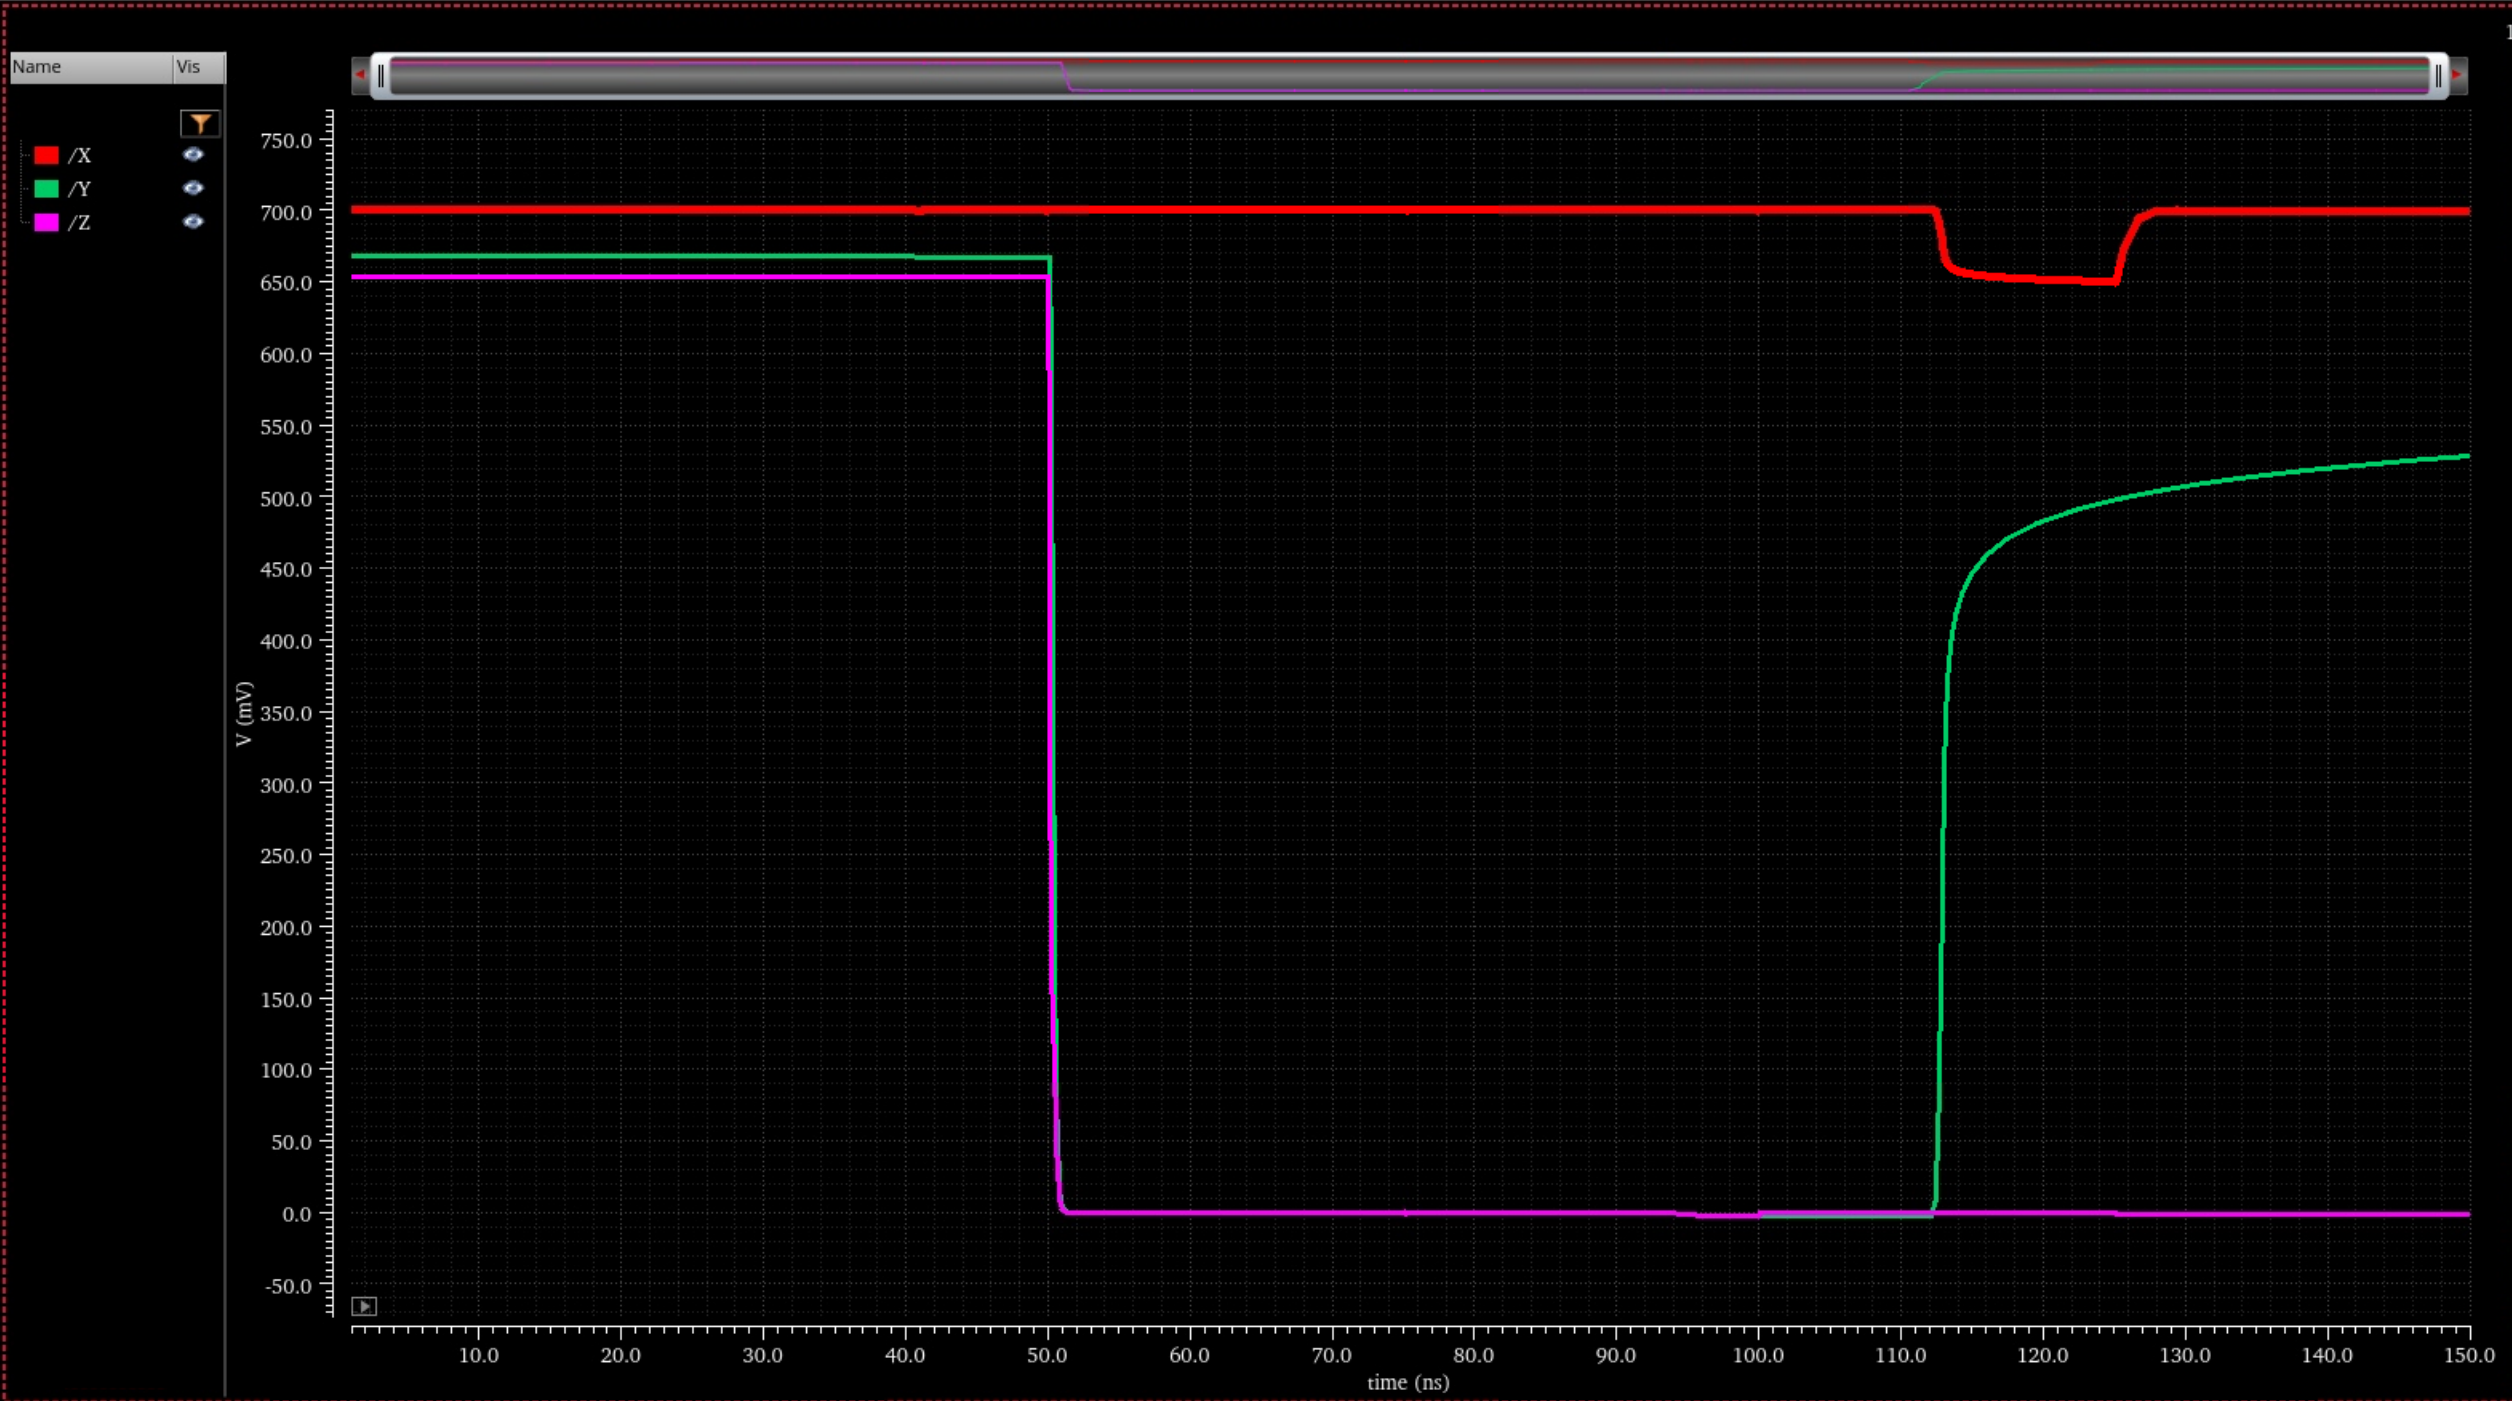
\includegraphics[width=0.50\textwidth]{Images/output_p1.png} 
    \caption{Problem 1.Input (left) and Ouput (right) Problem 1}
    \label{fid:input_output_p1}
\end{figure}

\clearpage

\section*{Problem 2}

\begin{figure}[h]
  \centering
  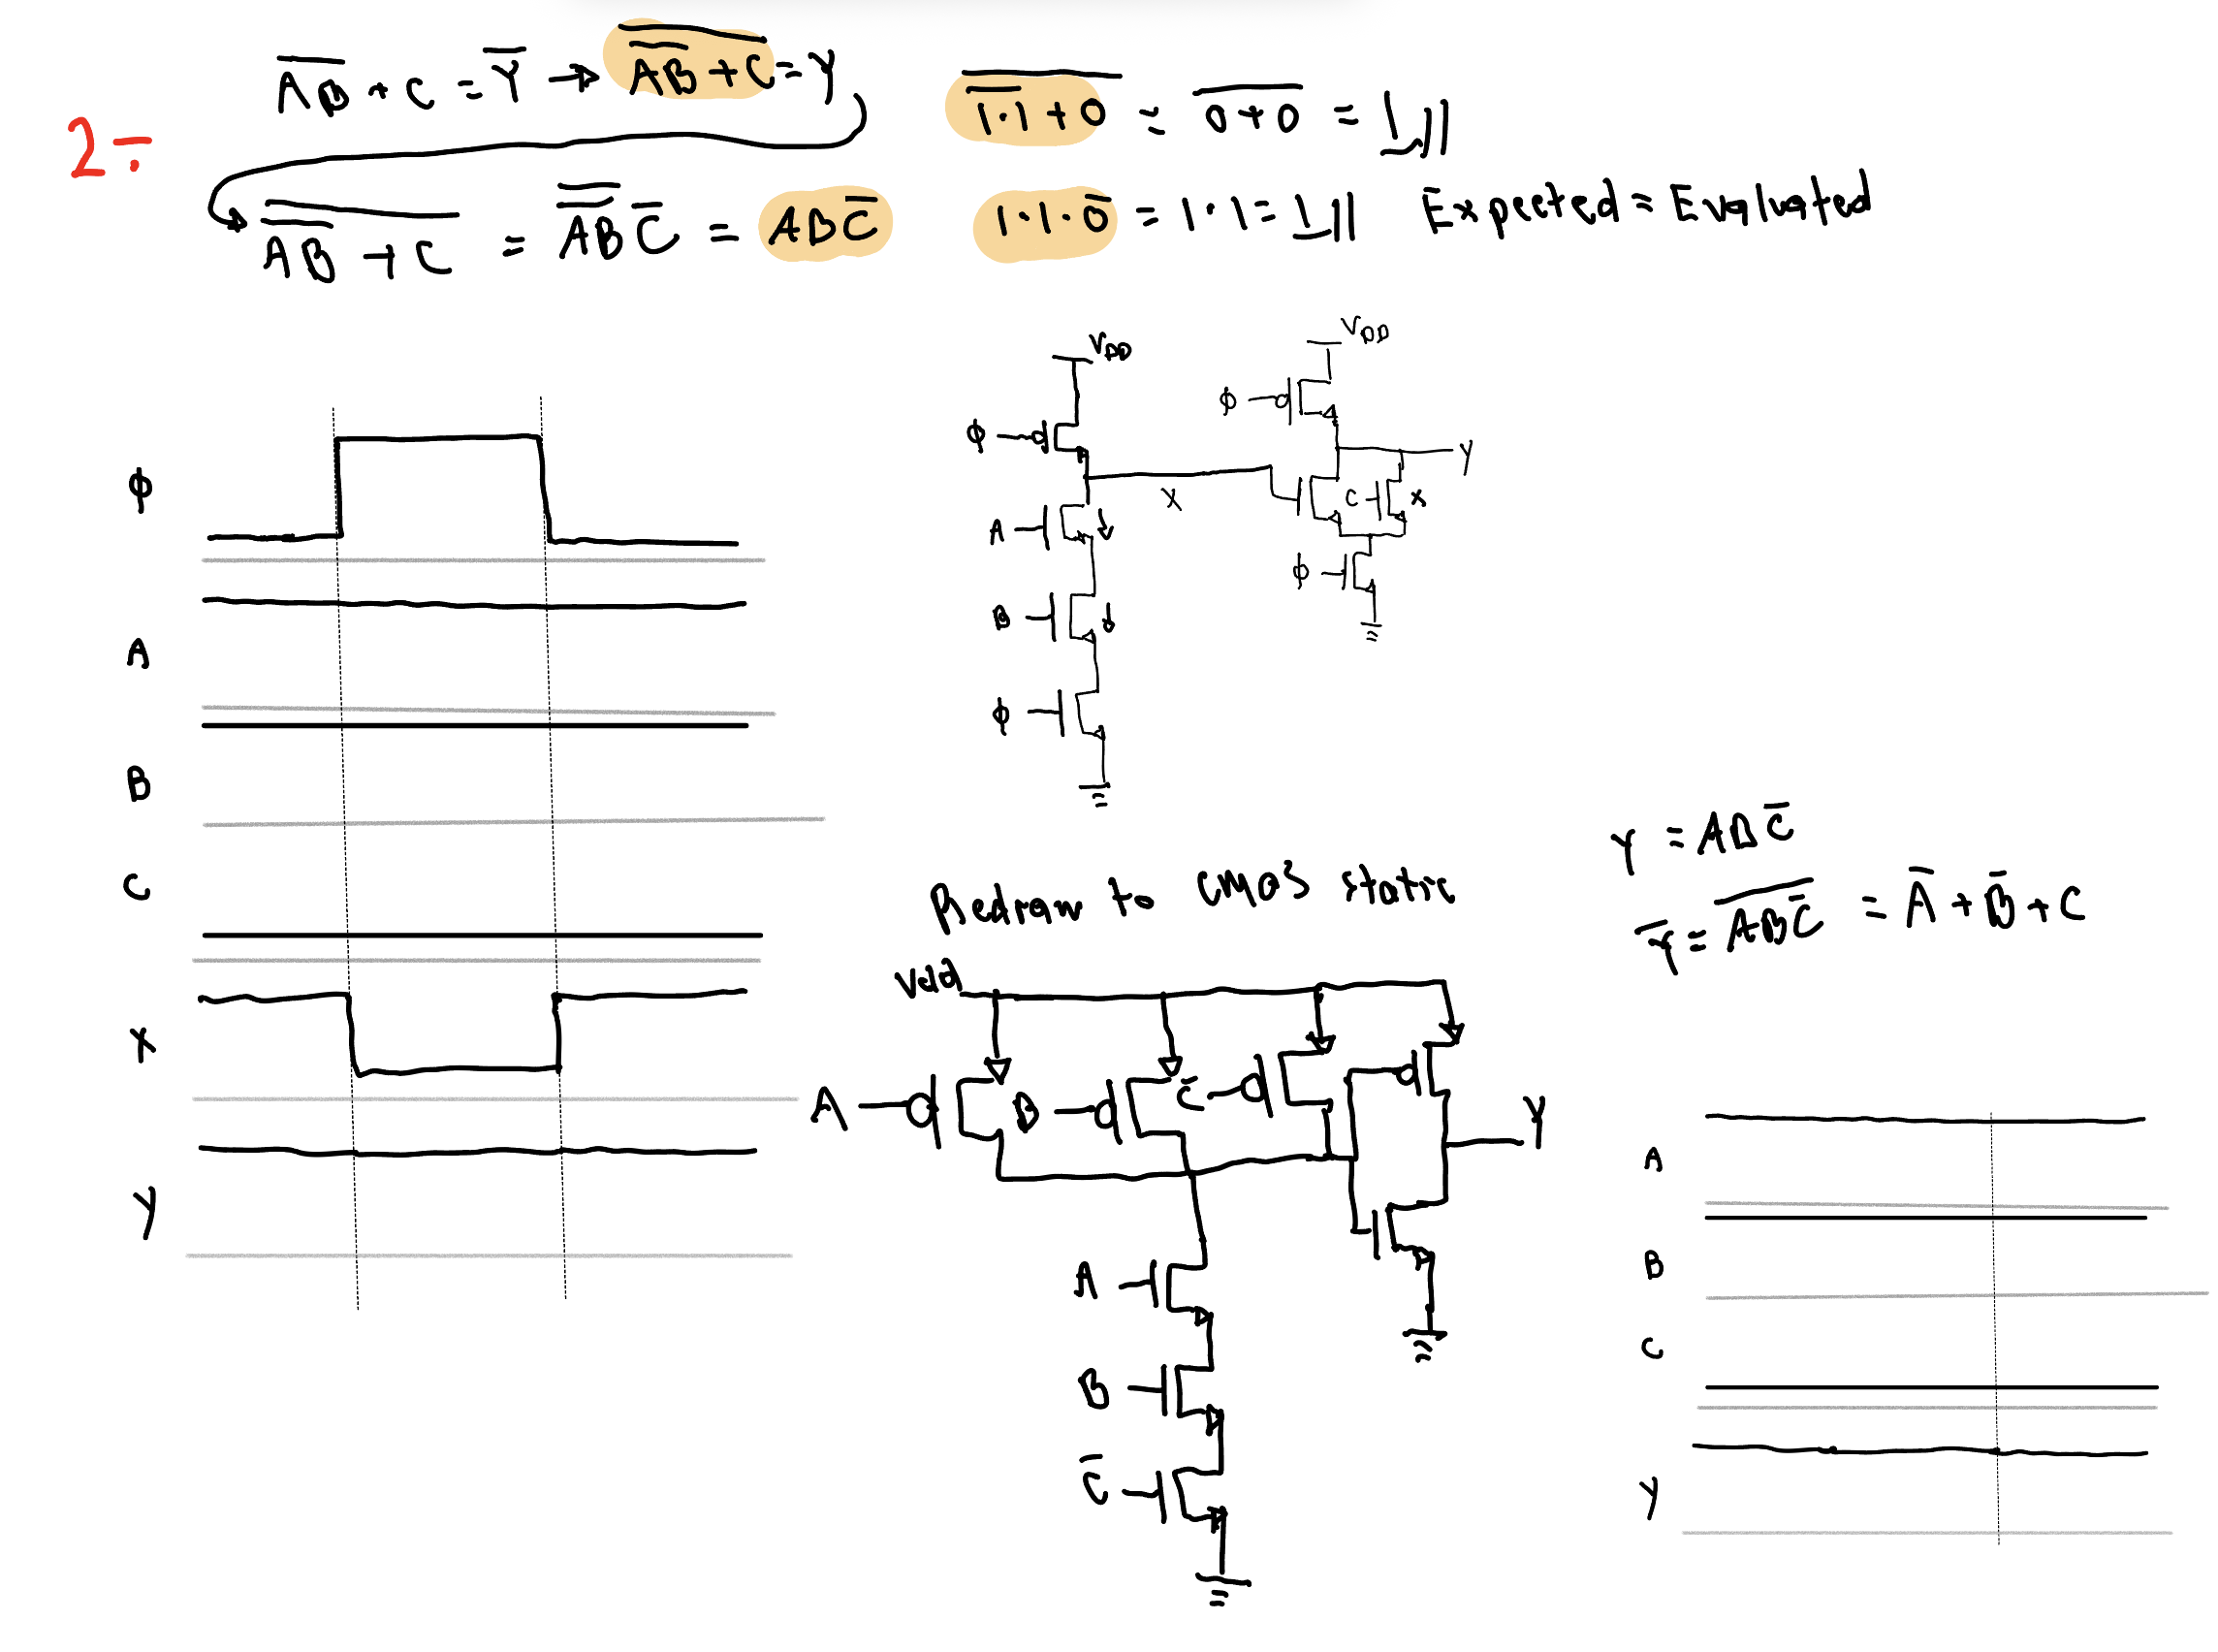
\includegraphics[width=0.80\linewidth, height=0.30\textheight, keepaspectratio]{Images/sketch_p2.png}
  \\[\smallskipamount]
  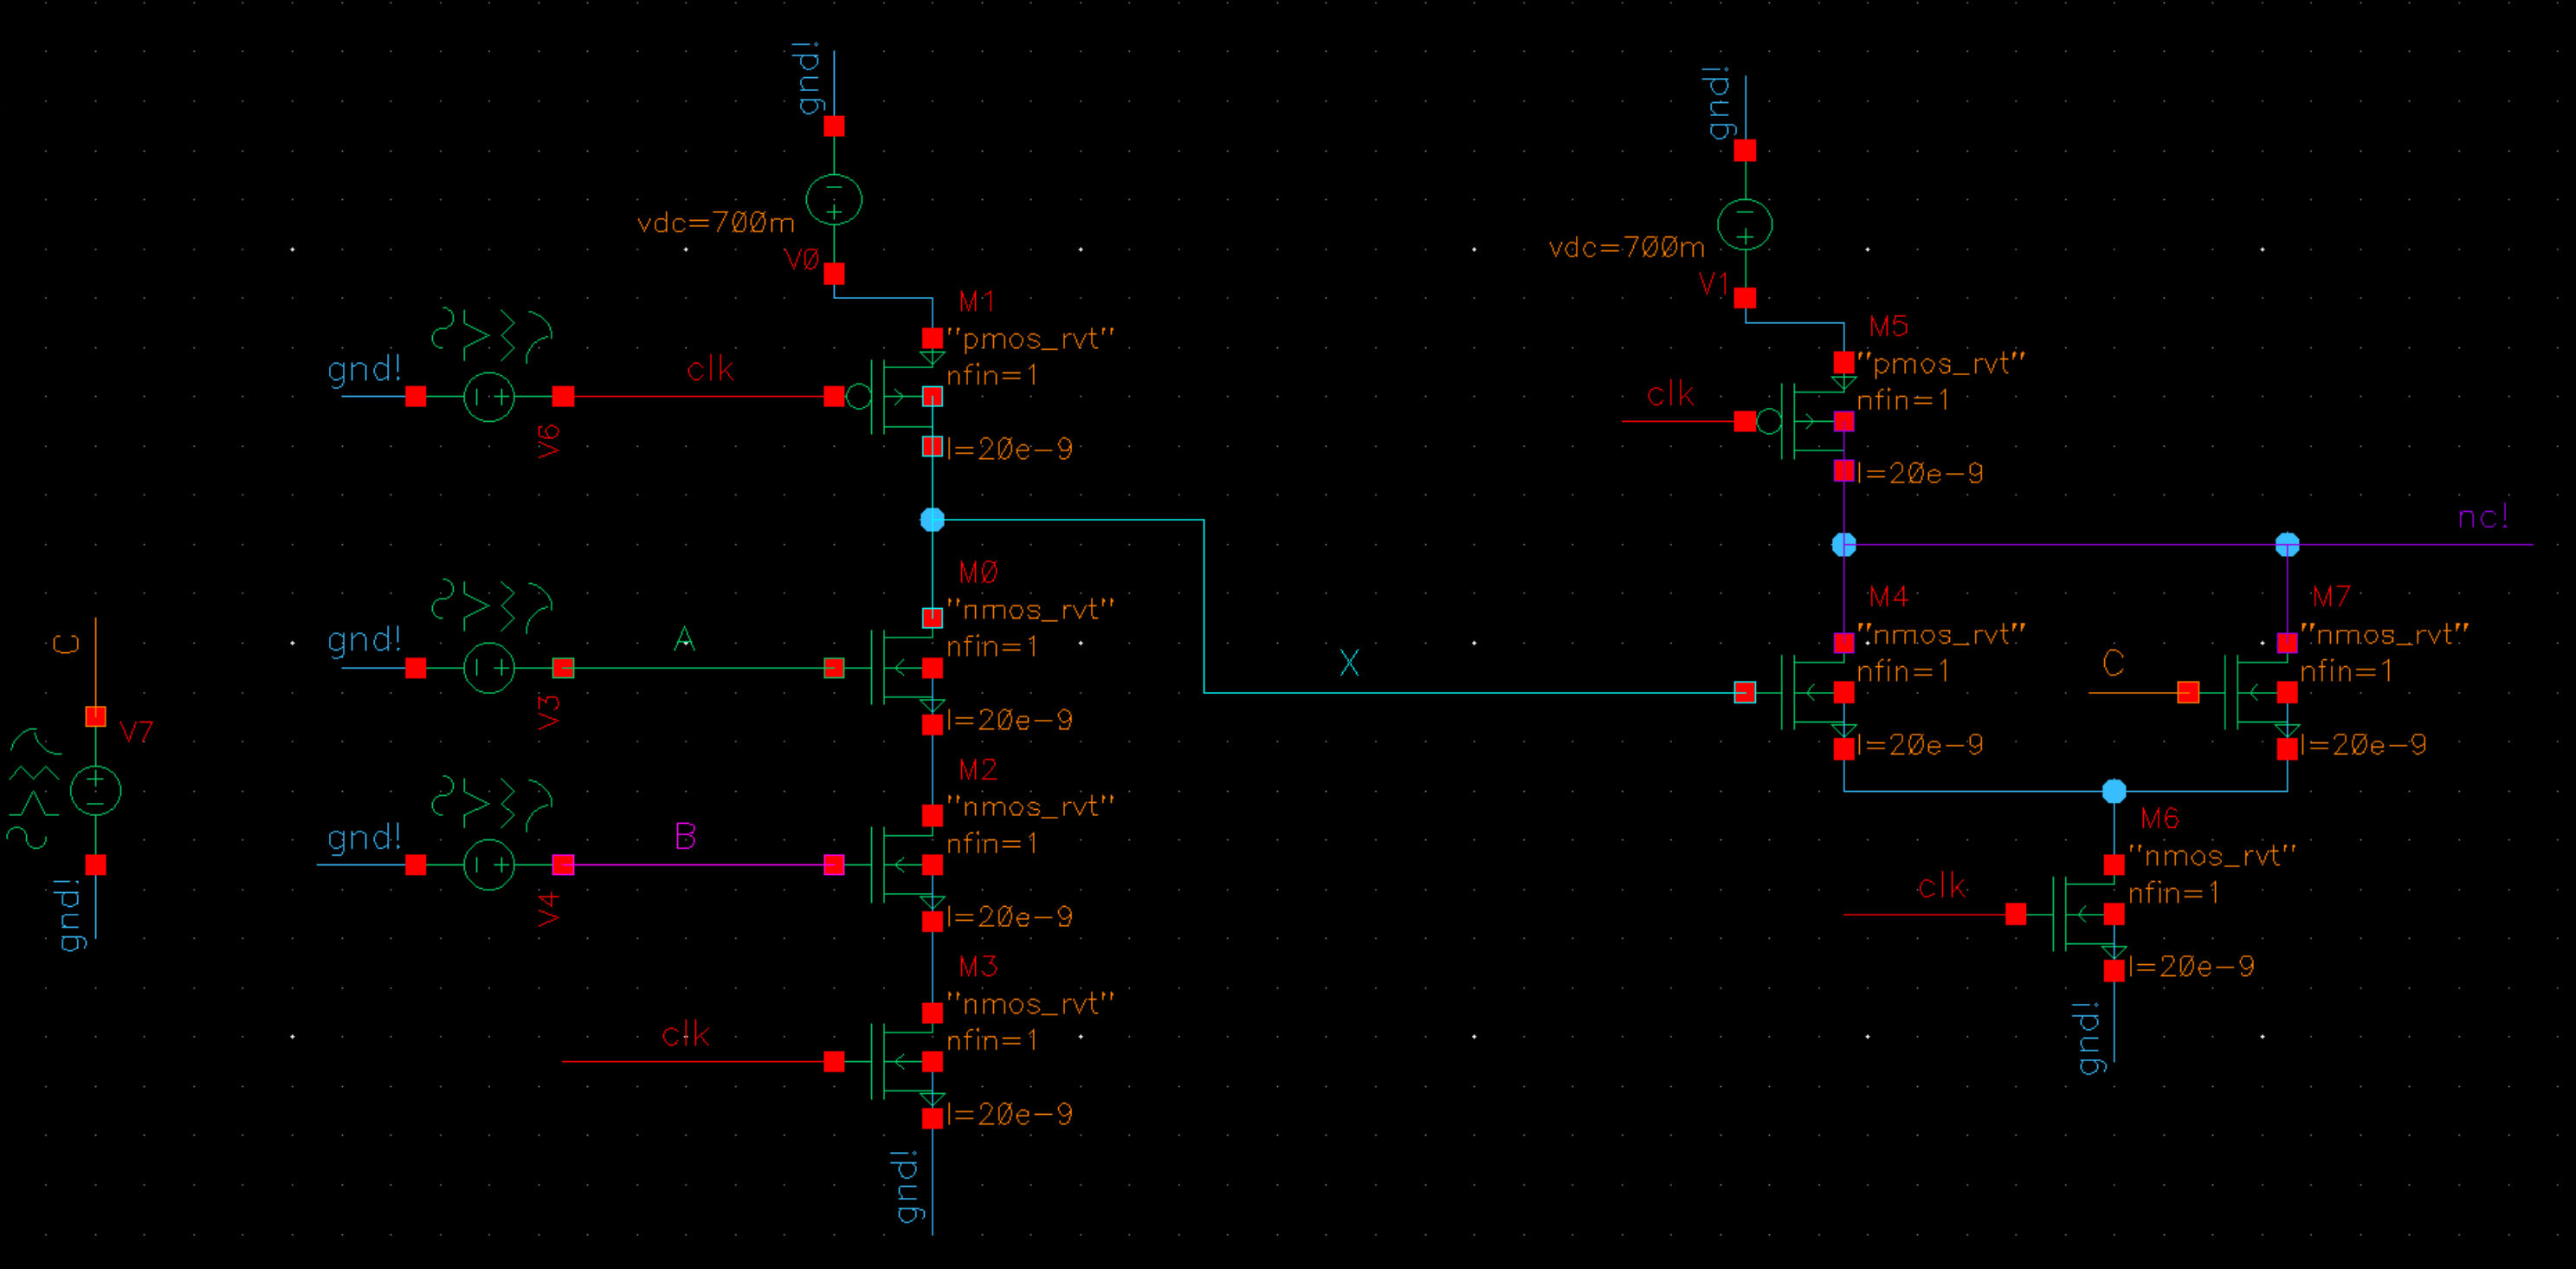
\includegraphics[width=0.45\linewidth, height=0.20\textheight, keepaspectratio]{Images/sch_p2.png}\hfill
  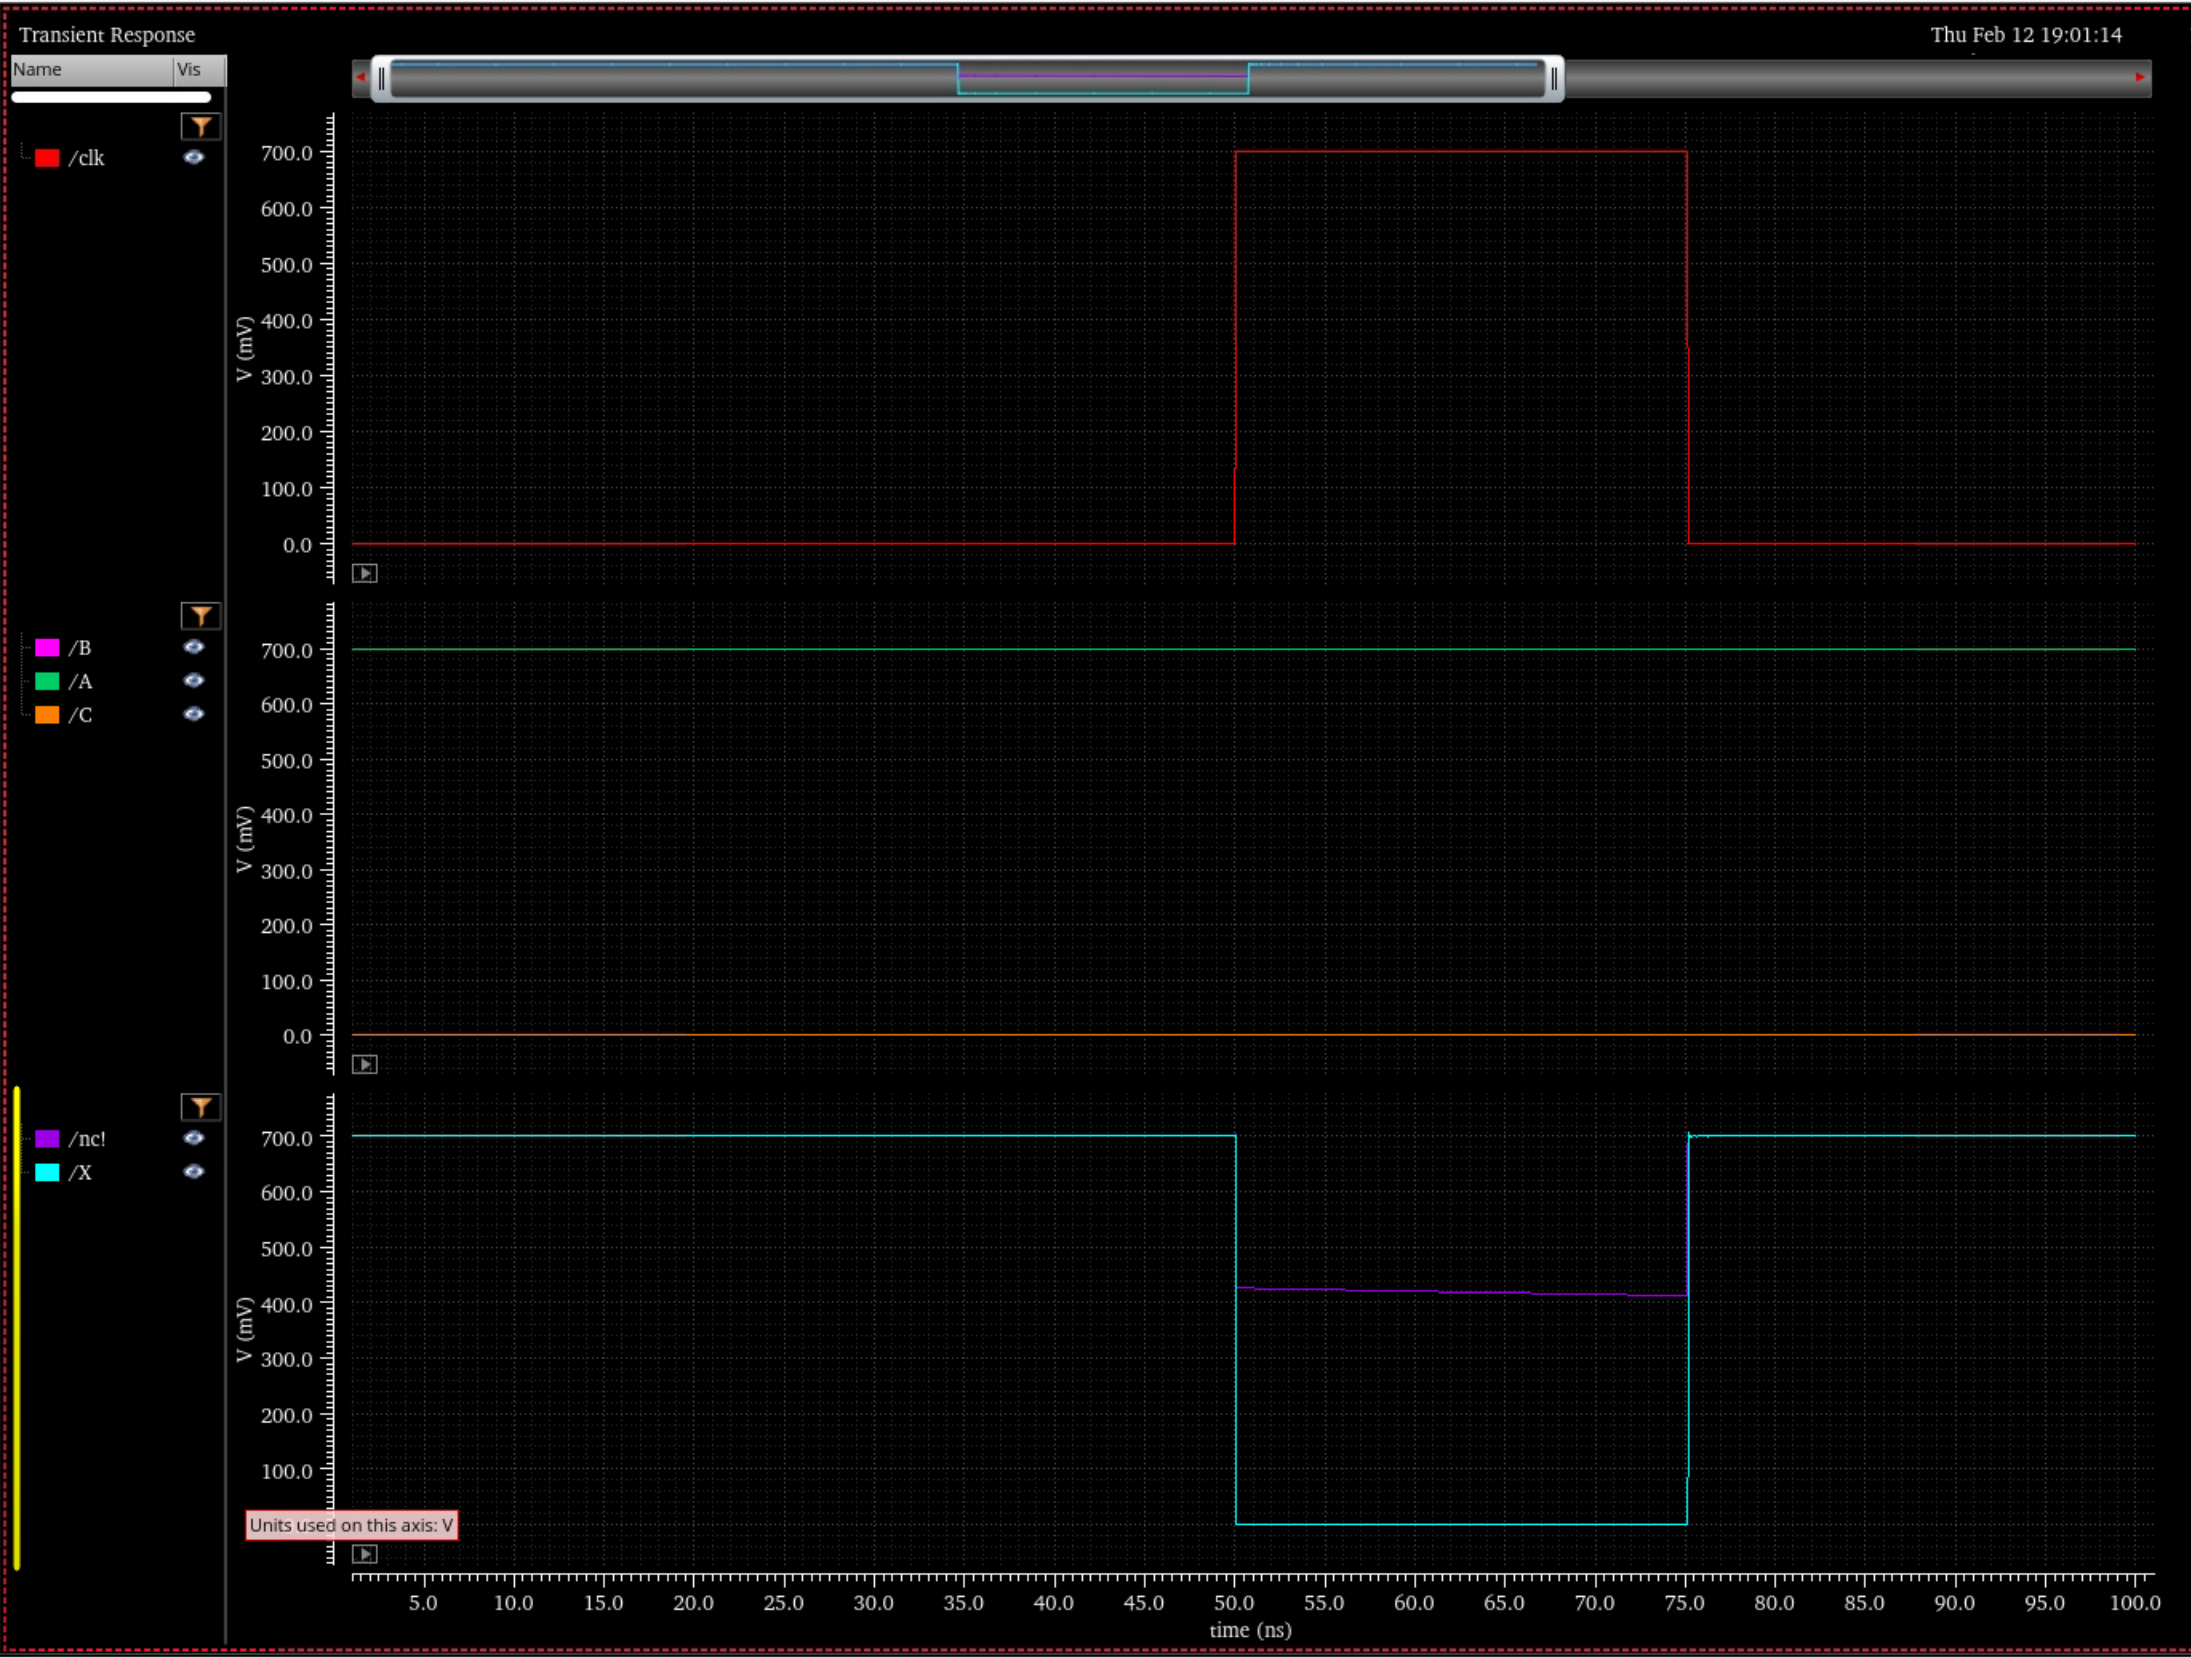
\includegraphics[width=0.54\linewidth, height=0.20\textheight, keepaspectratio]{Images/output_p2.png}
  \\[\smallskipamount]
  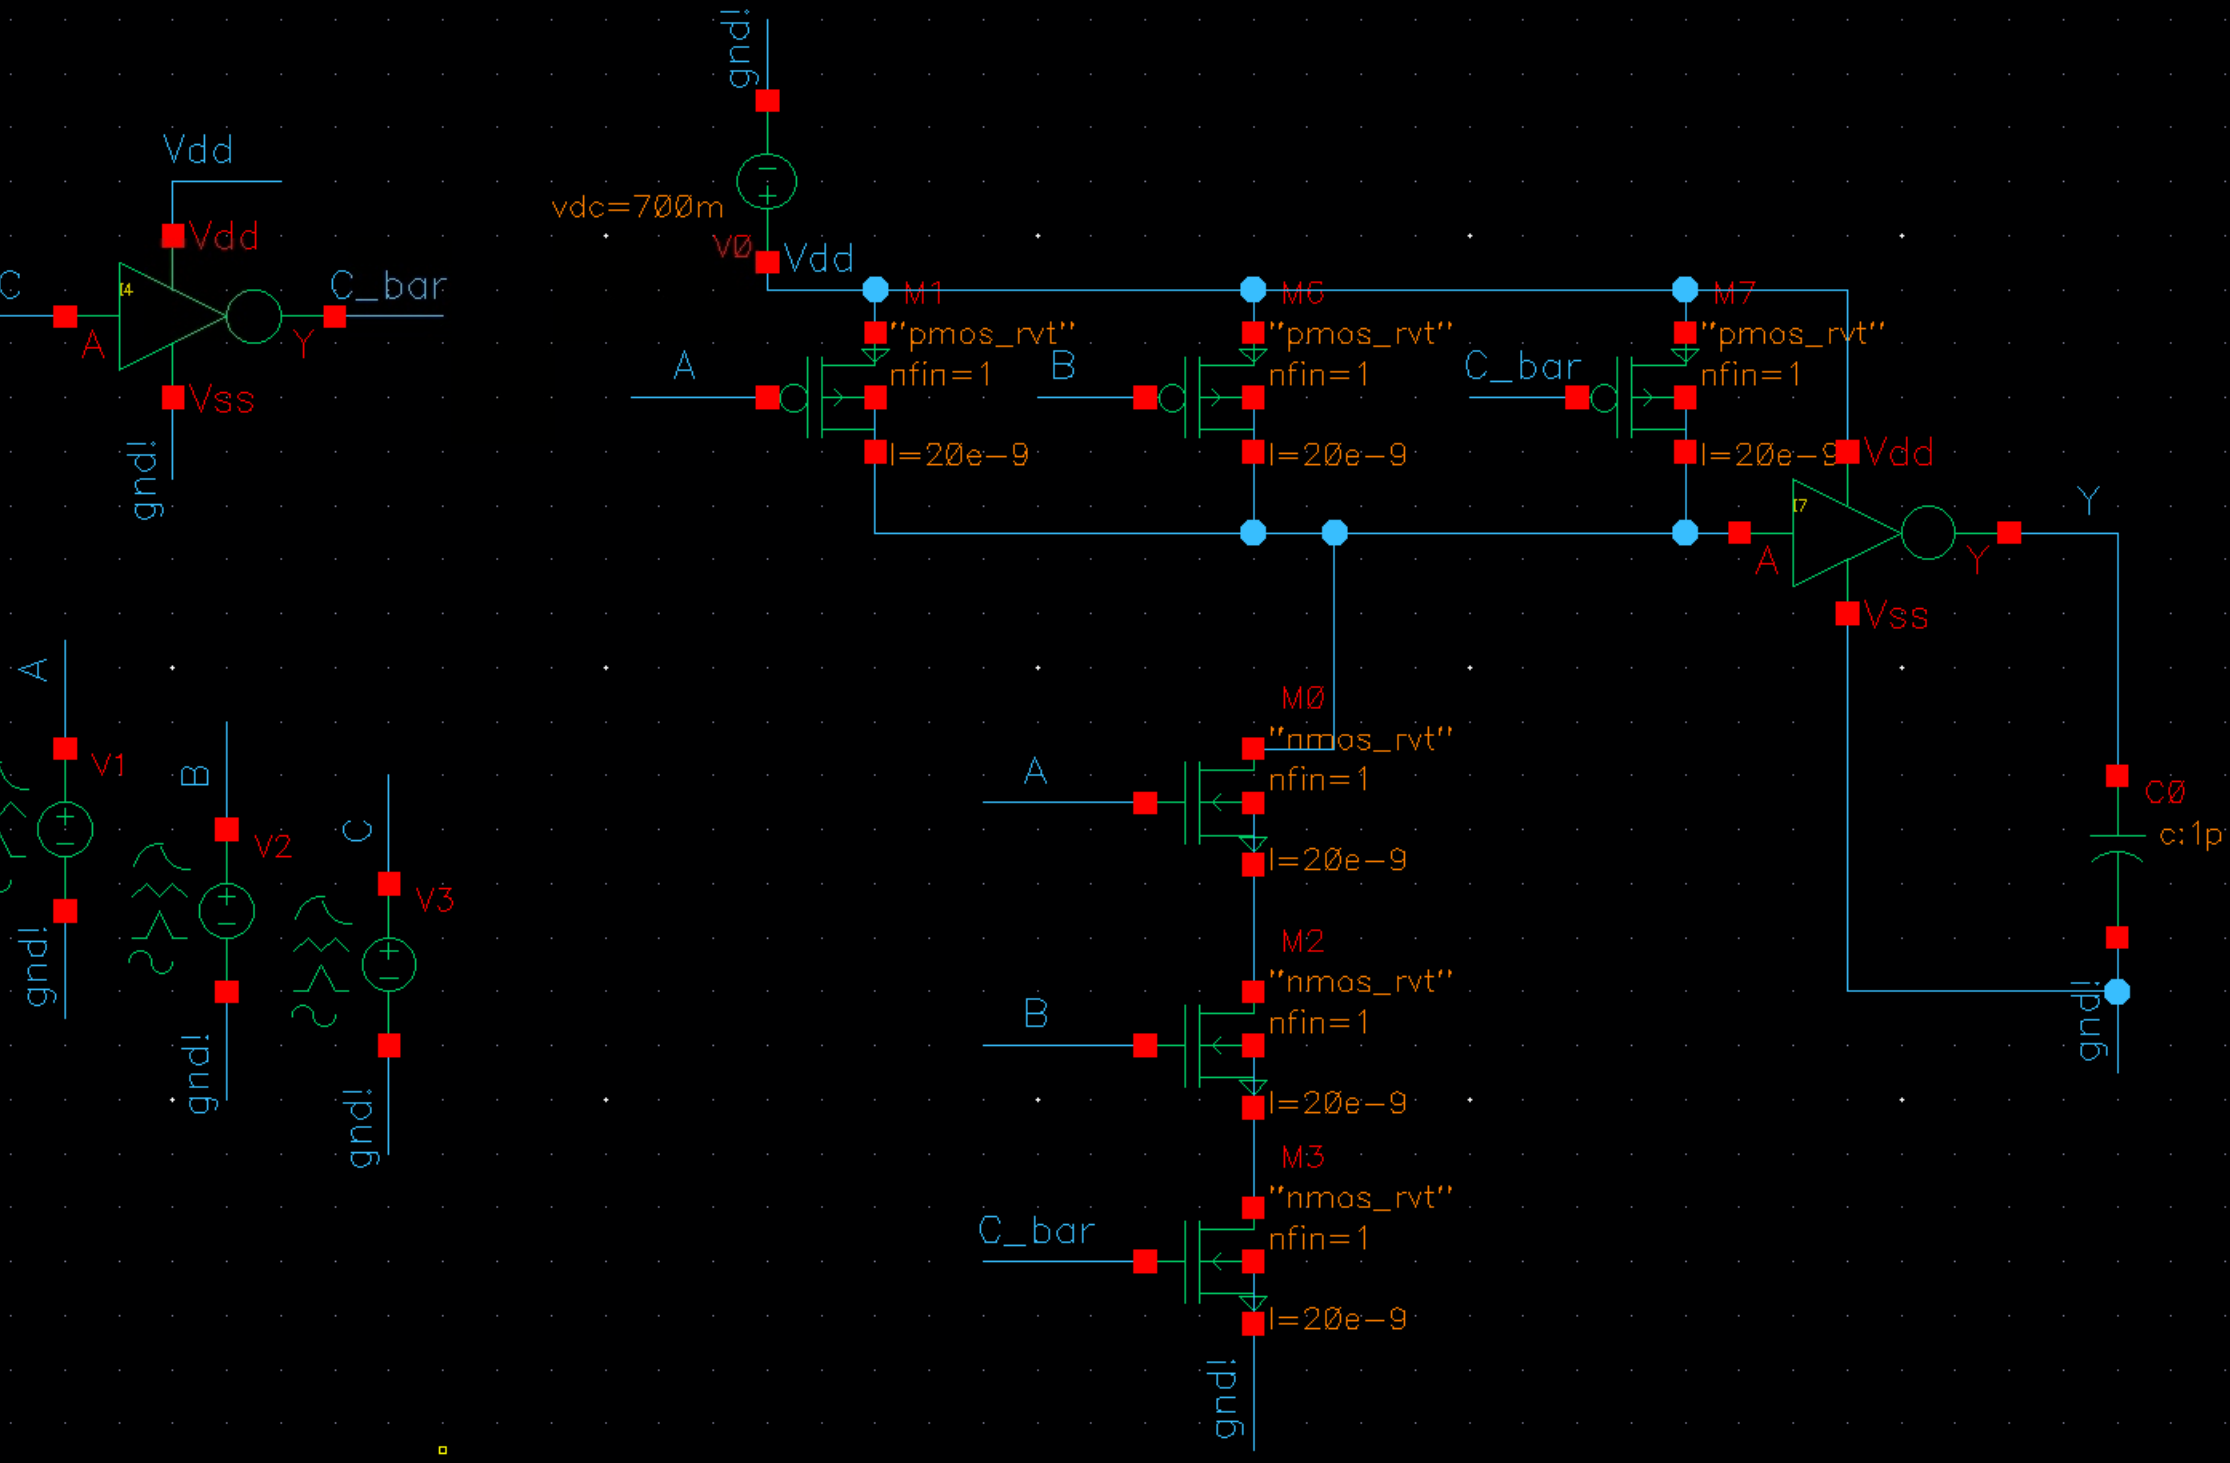
\includegraphics[width=0.45\linewidth, height=0.20\textheight, keepaspectratio]{Images/sch_b_p2.png}\hfill
  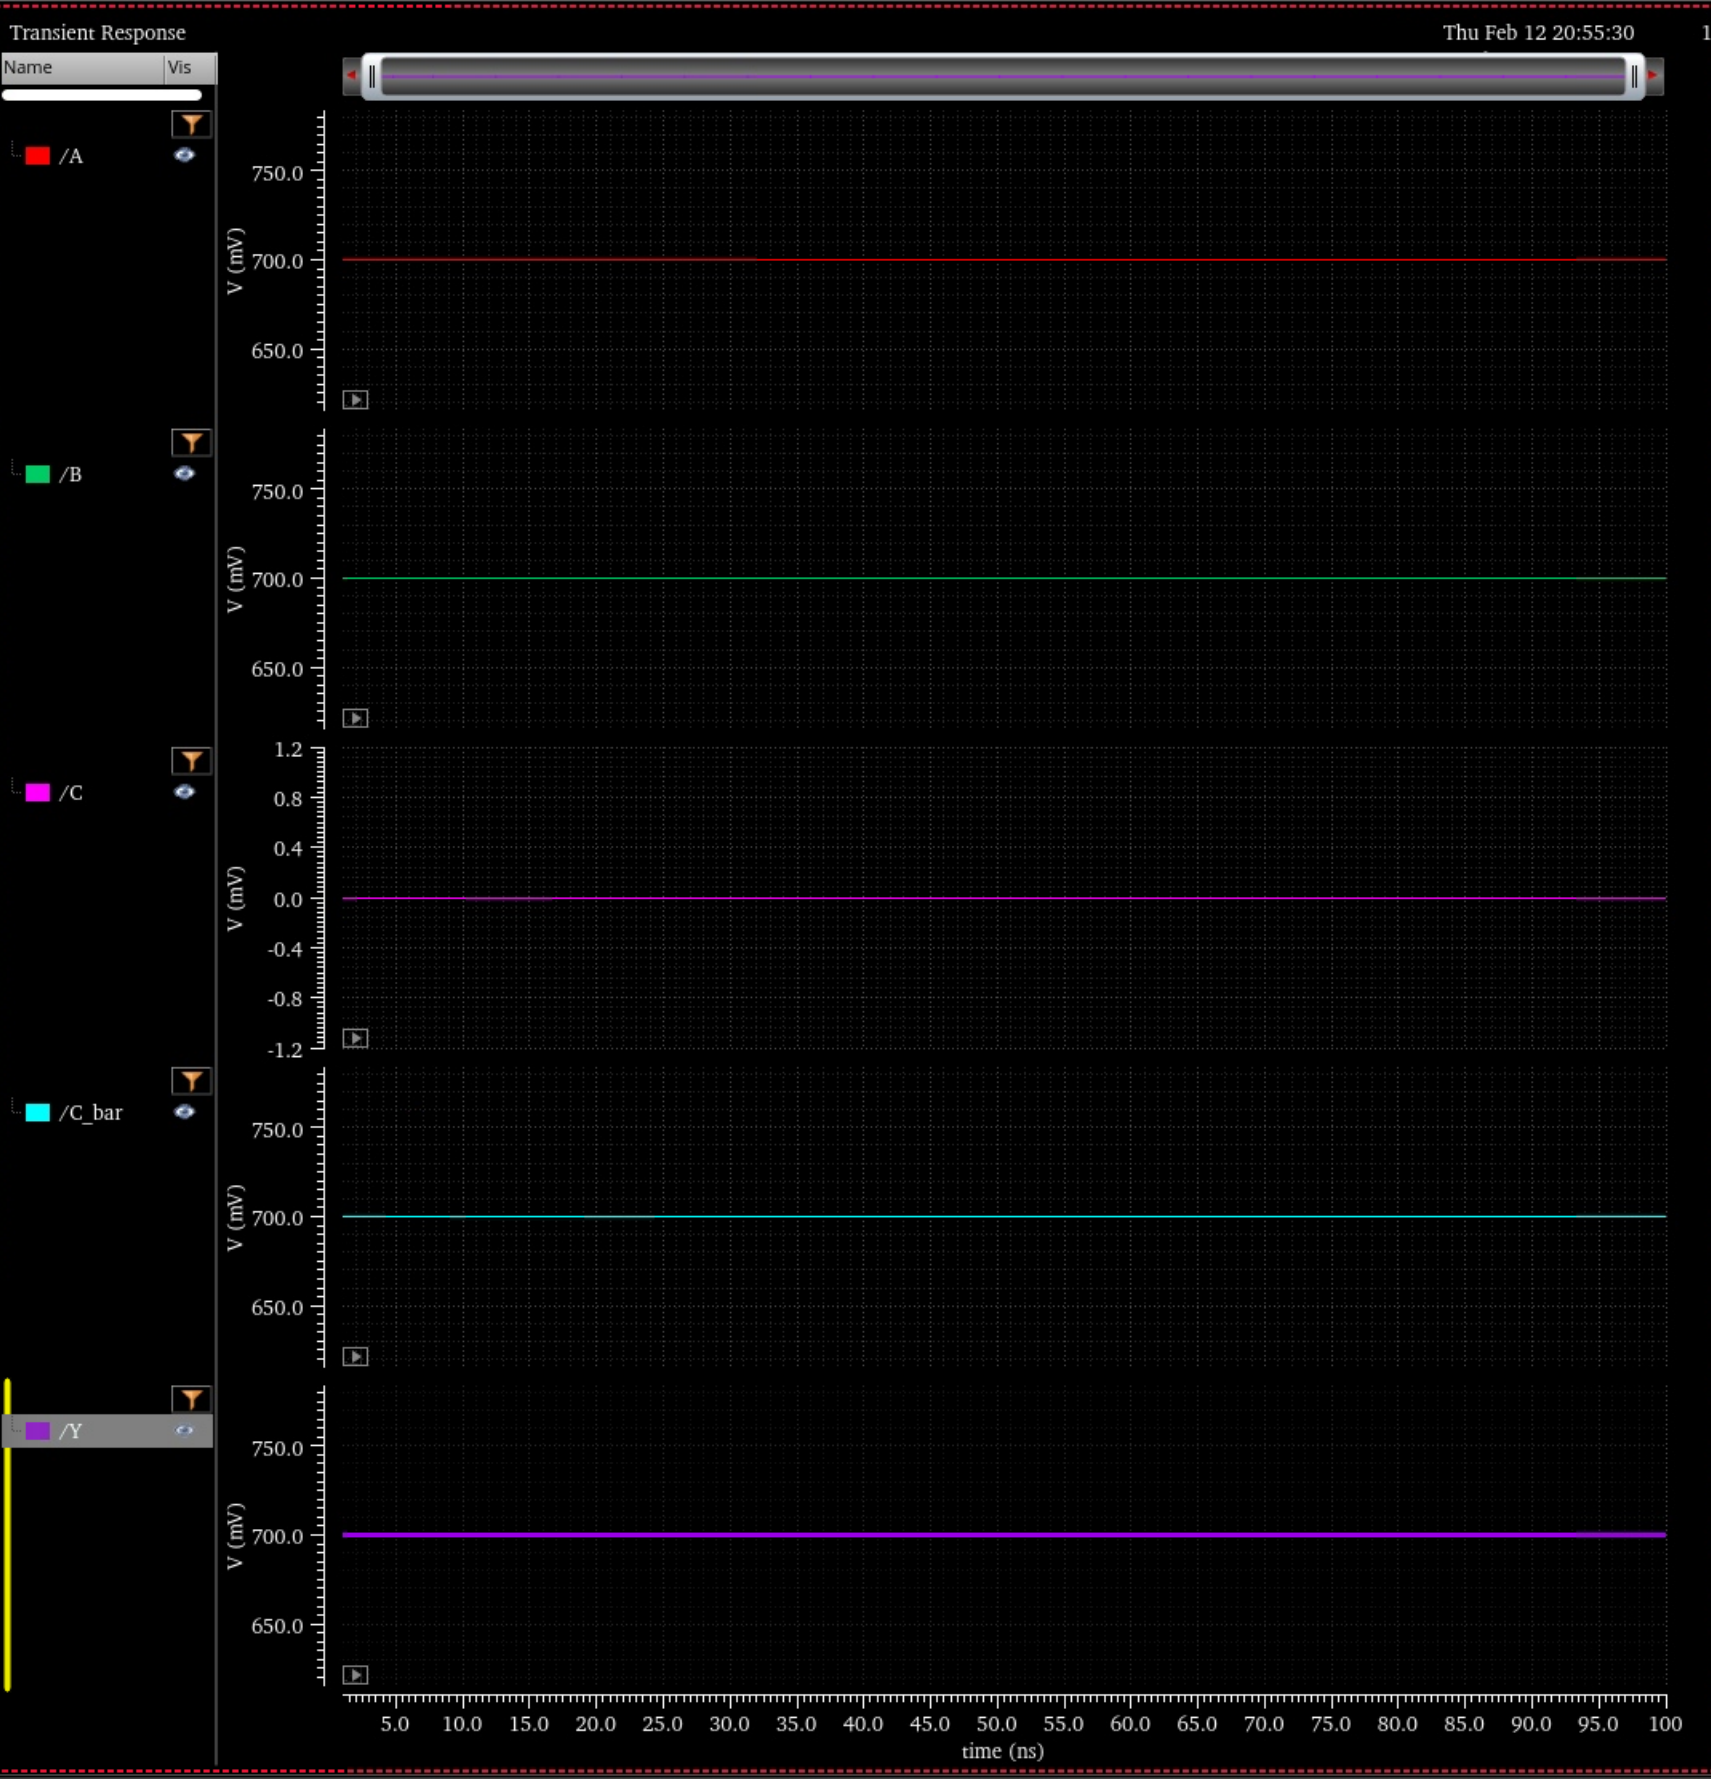
\includegraphics[width=0.54\linewidth, height=0.20\textheight, keepaspectratio]{Images/output_b_p2.png}
  \caption{Problem 2. First row sketch. Second row dynamic logic. Third row static logic.}
  \label{fid:output_p2}
\end{figure}

\clearpage

\section*{Problem 3}

\begin{figure}[h]
  \centering
  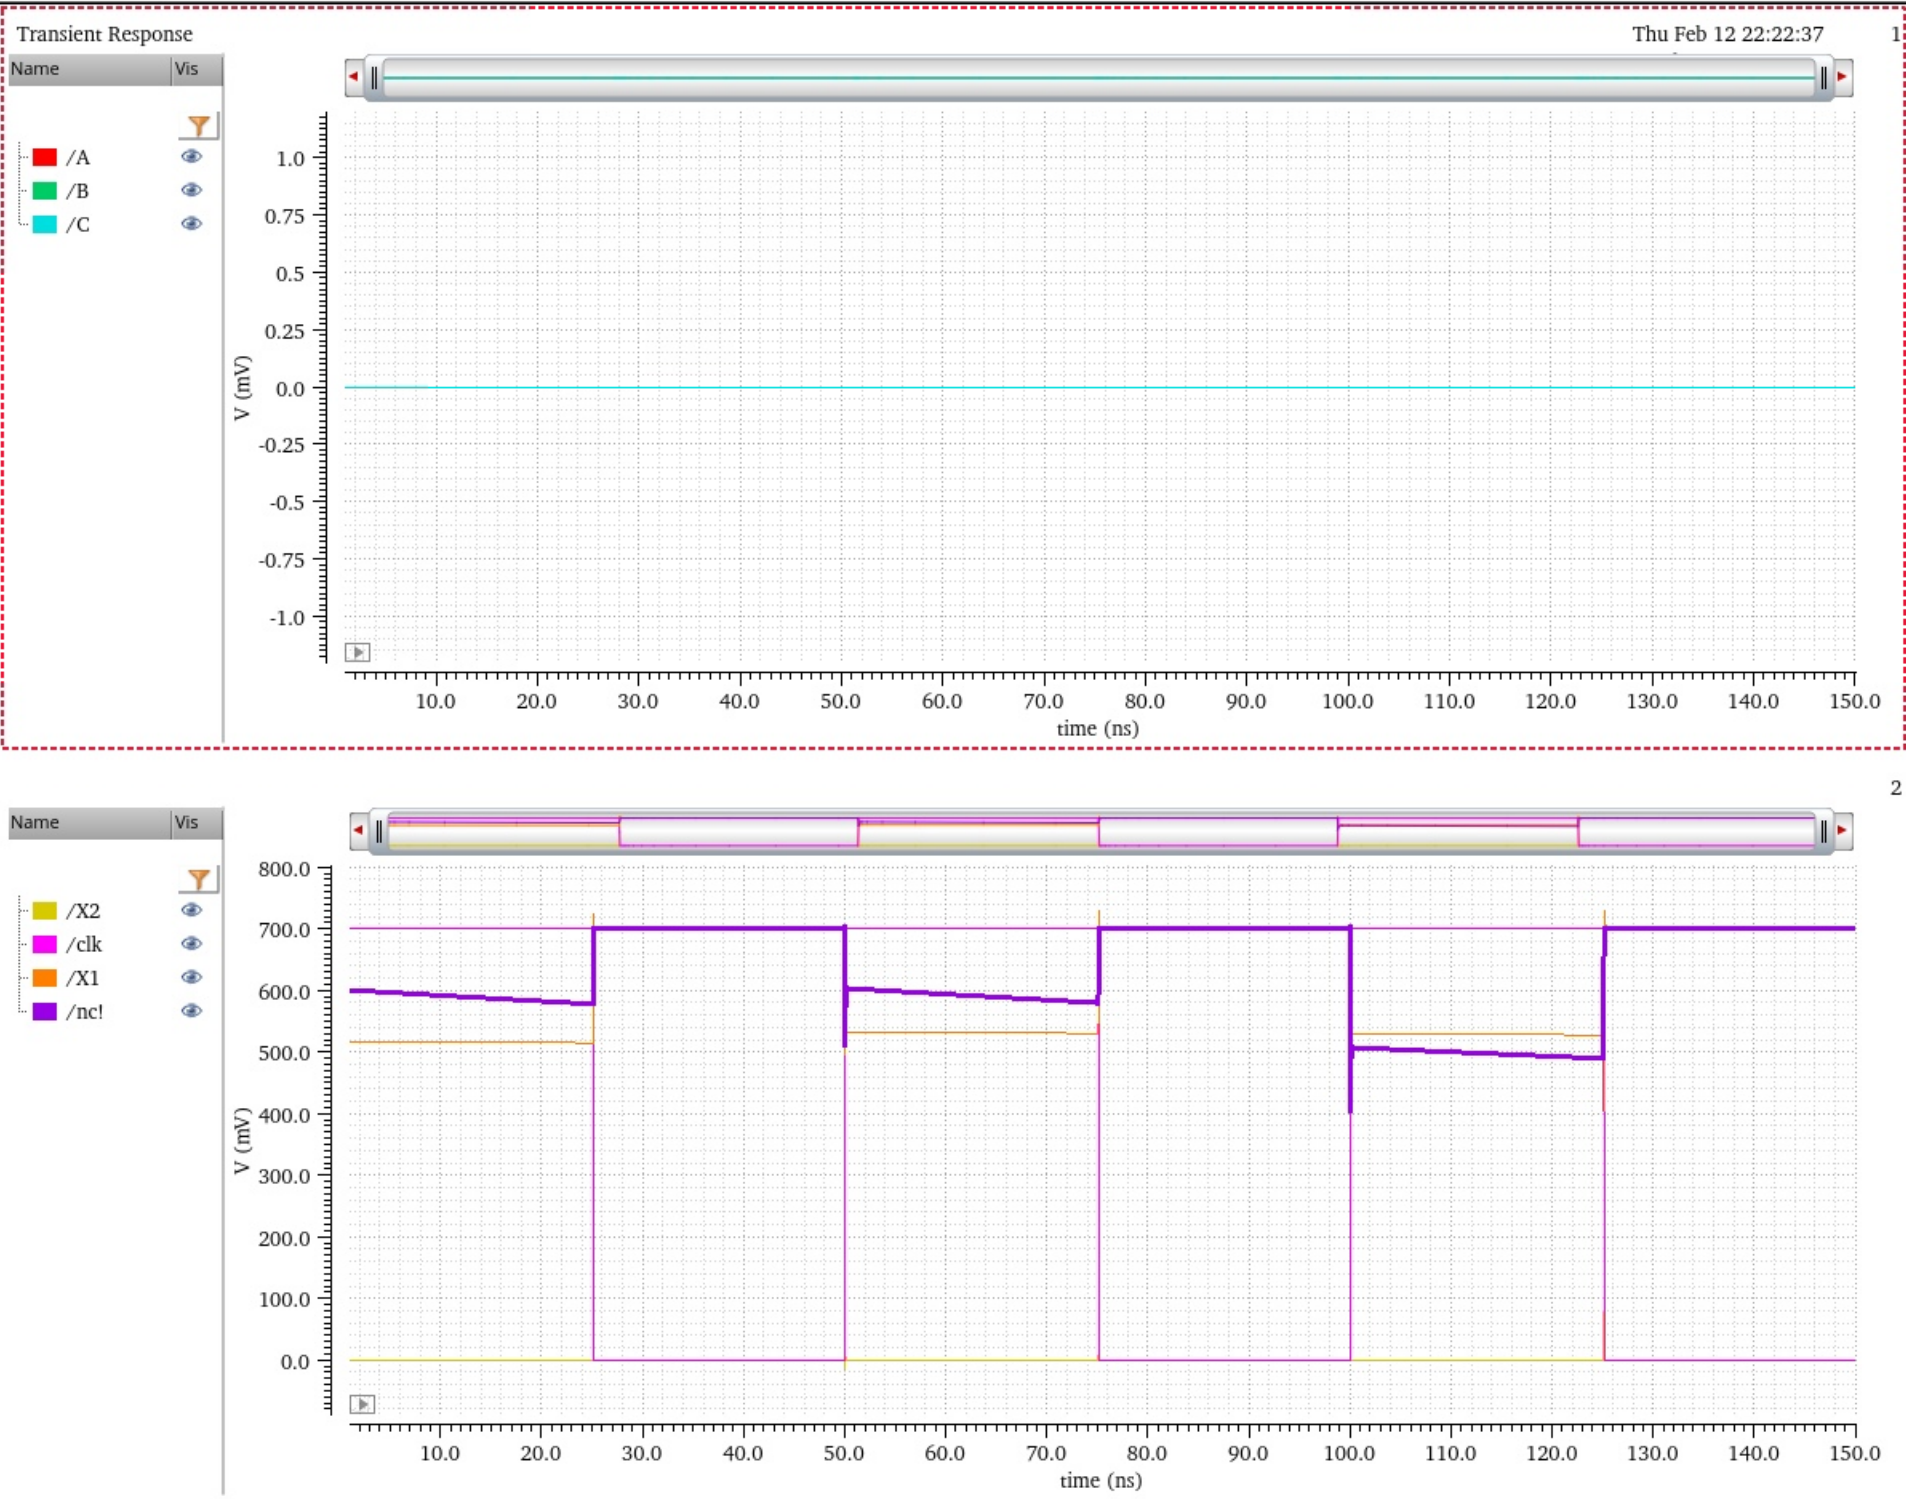
\includegraphics[width=0.45\linewidth, height=0.20\textheight, keepaspectratio]{Images/output_p3_000_1.png}\hfill
  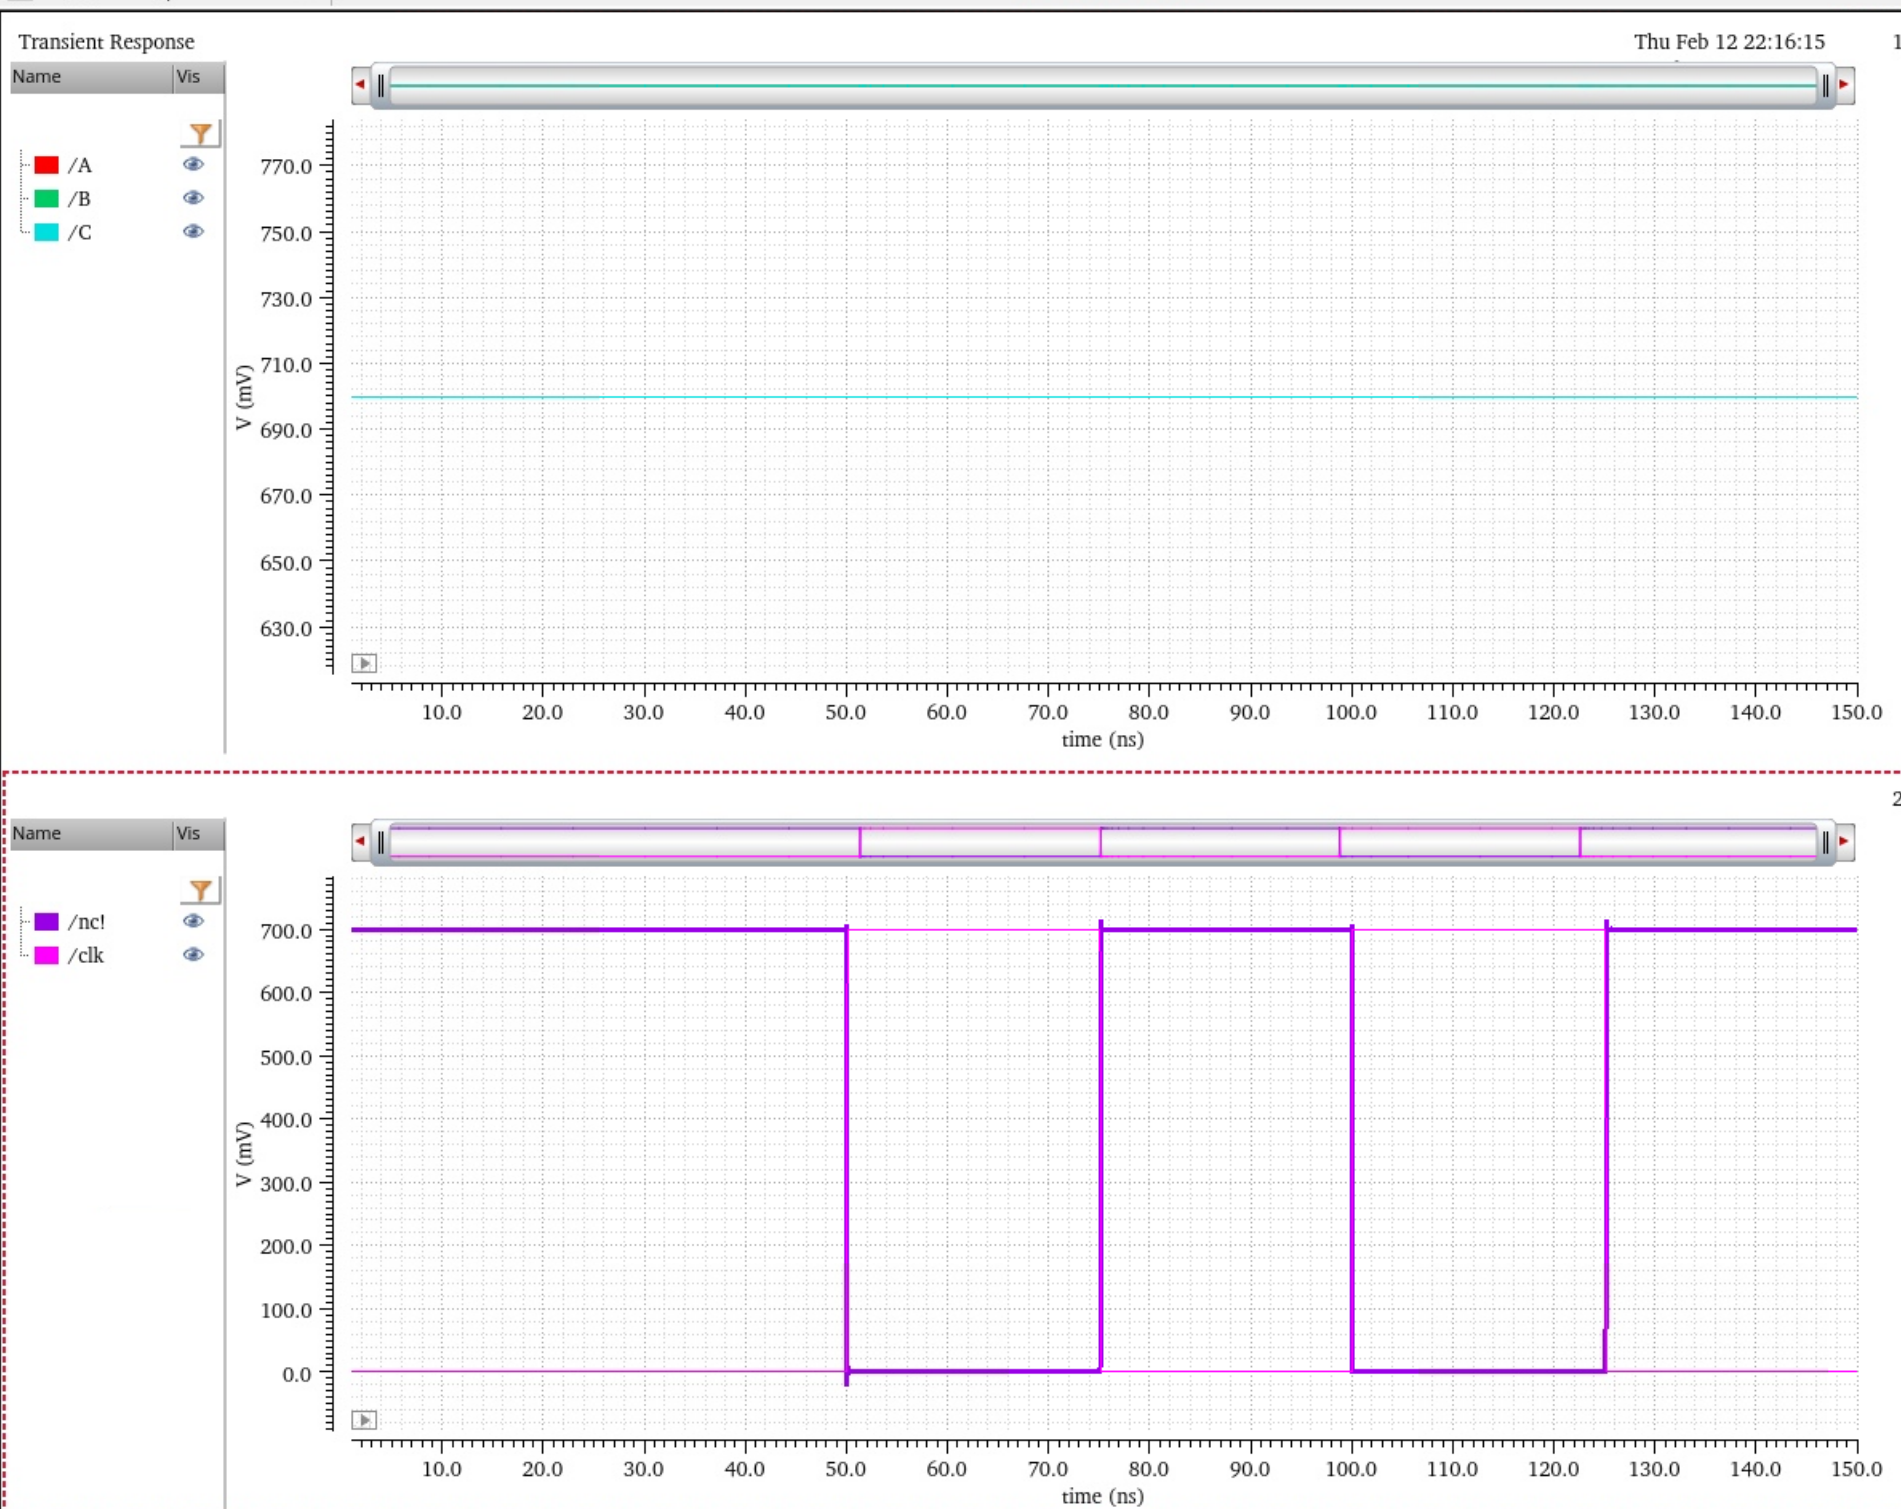
\includegraphics[width=0.54\linewidth, height=0.20\textheight, keepaspectratio]{Images/output_p3_111_1.png}
  \\[\smallskipamount]
  \centering
  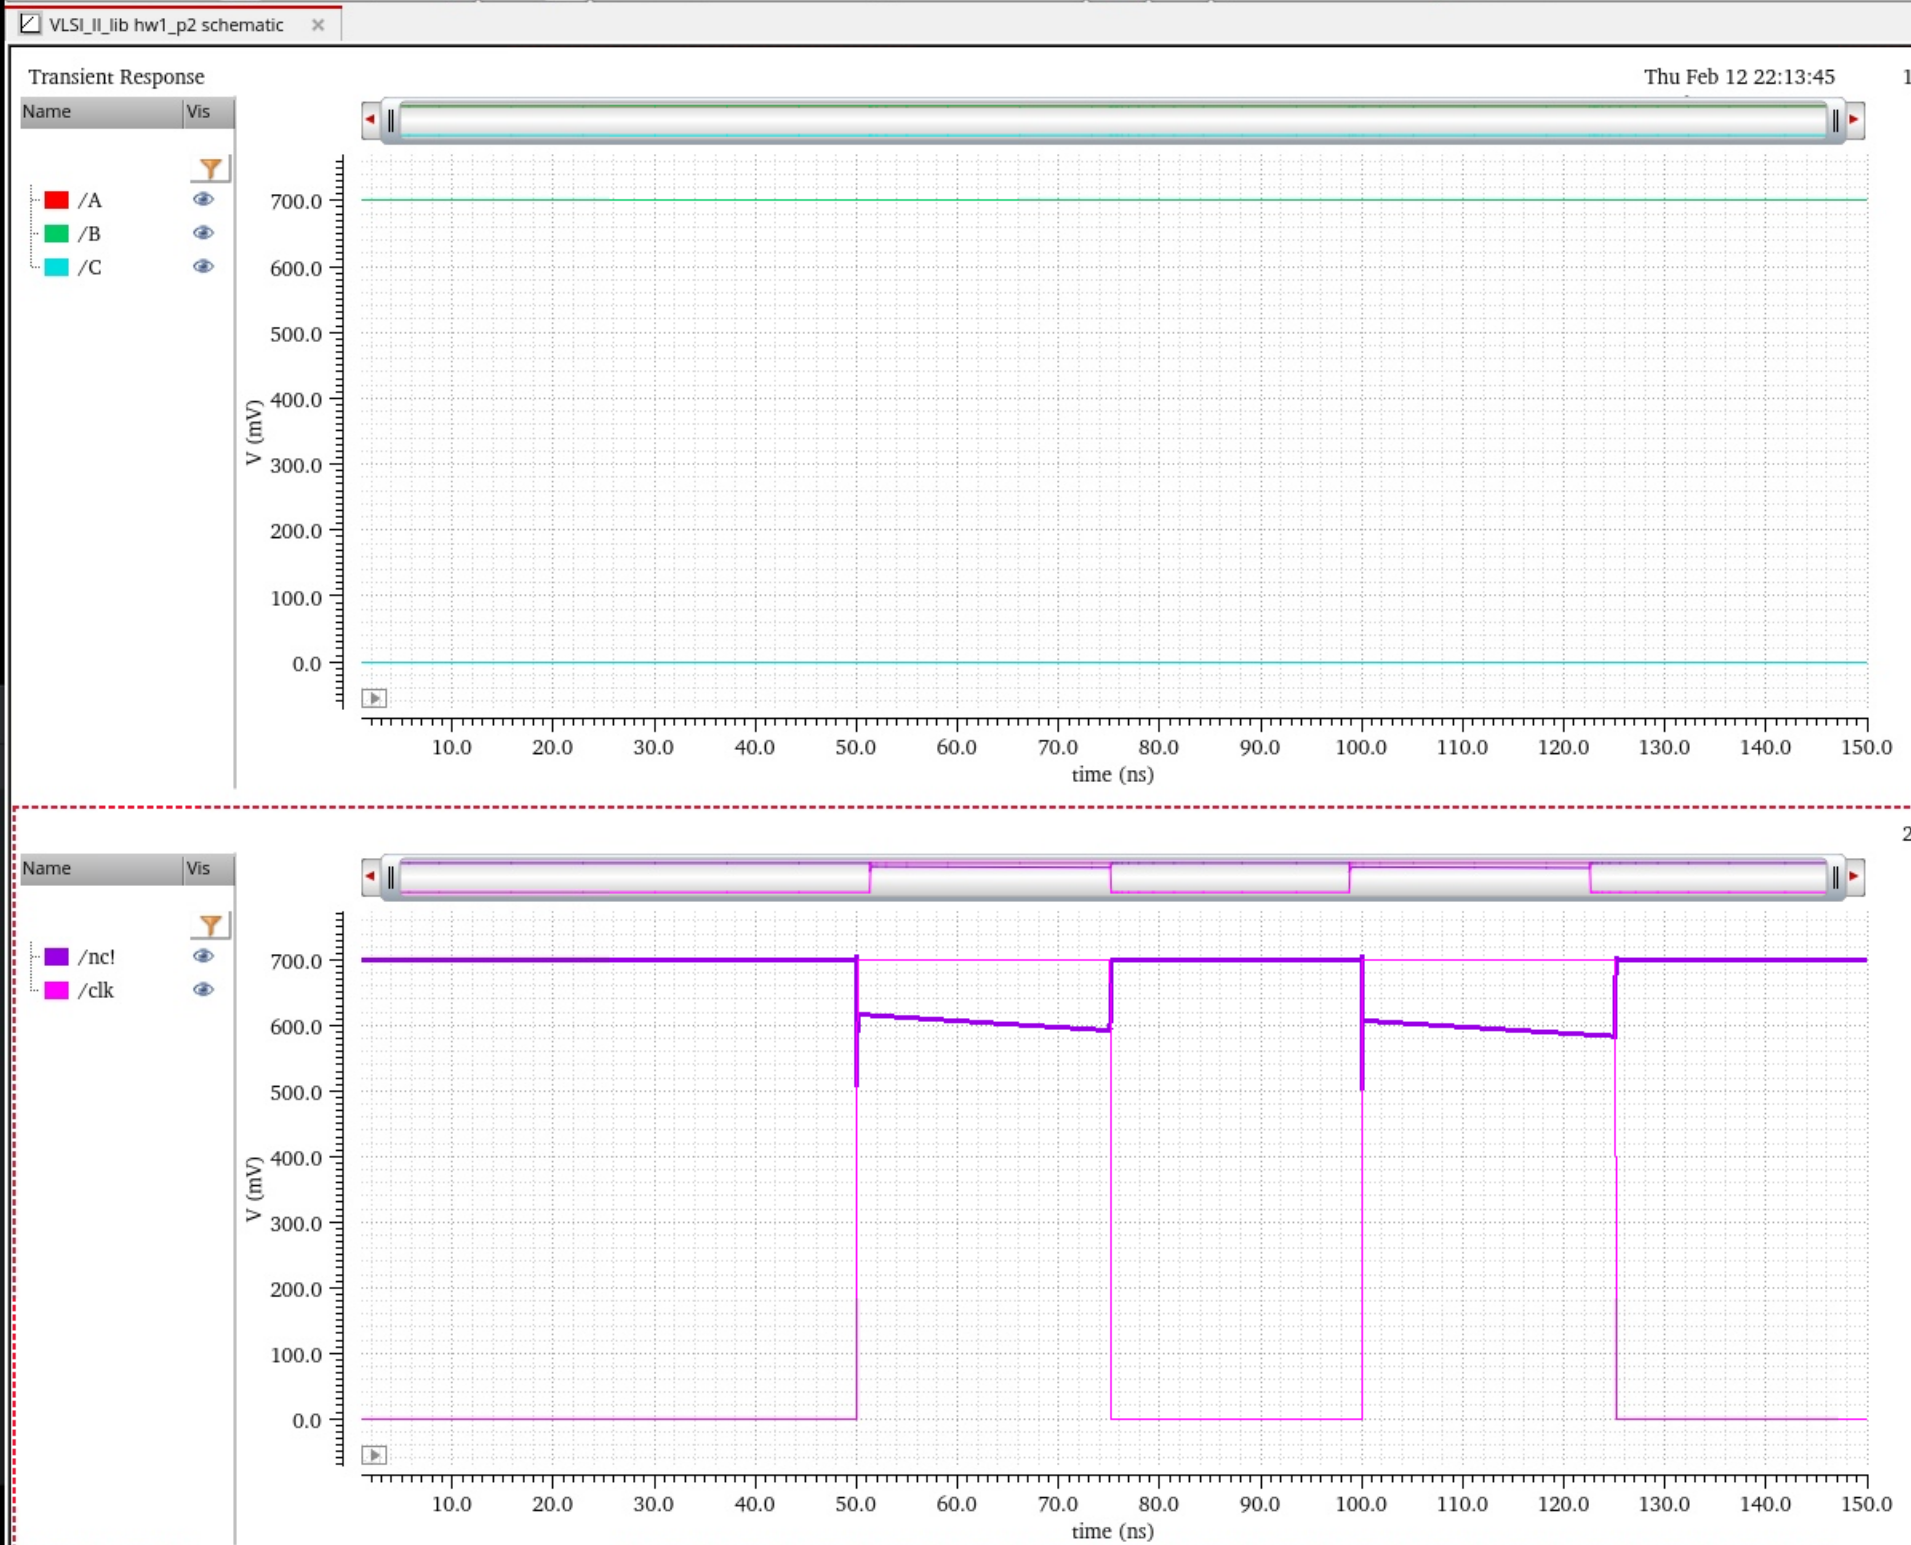
\includegraphics[width=0.45\linewidth, height=0.20\textheight, keepaspectratio]{Images/output_p3_110_1.png}\hfill
  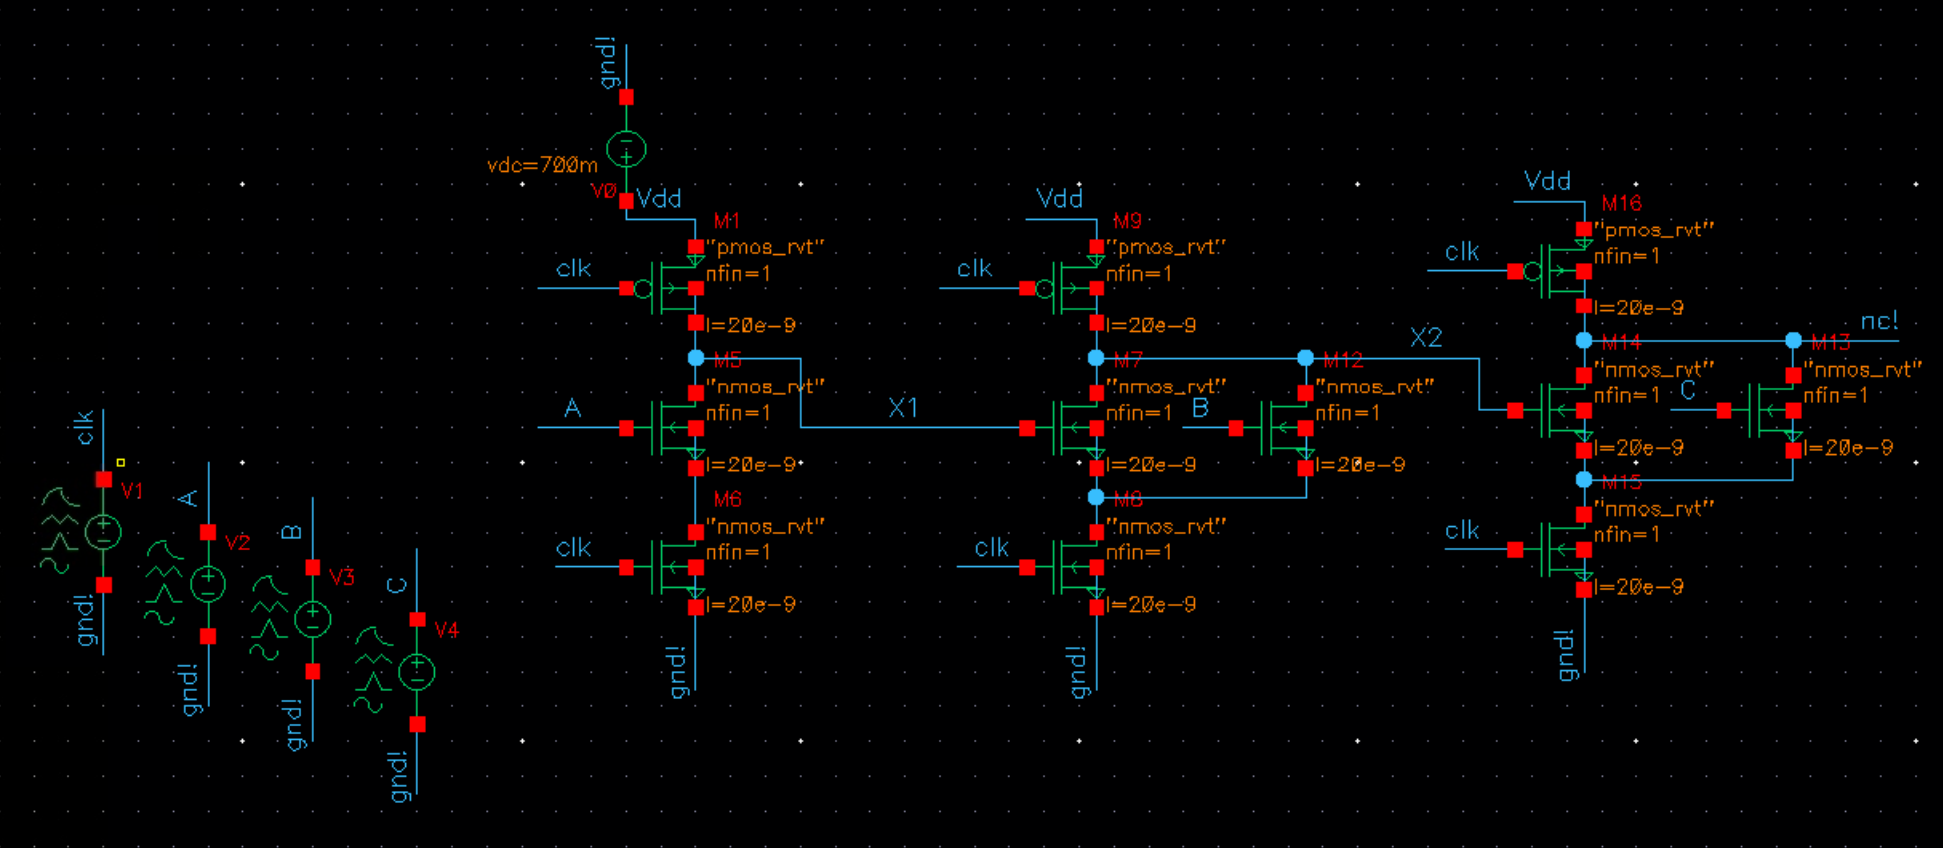
\includegraphics[width=0.45\linewidth, height=0.20\textheight, keepaspectratio]{Images/sch_p3_1.png}\hfill
  \caption{Problem 3. Top left 000. Top right 111. Bottom left 110. Bottom right schematic.}
  \label{fid:output_p3_1}
  \parbox{\linewidth}{Output of F=A+B+C. Error in input 000. Output is 1 instead of 0. When all inputs are logic 1. The Output (nc) has to discharge and charge with every clk cycle.}
\end{figure}



\begin{figure}[h]
  \centering
  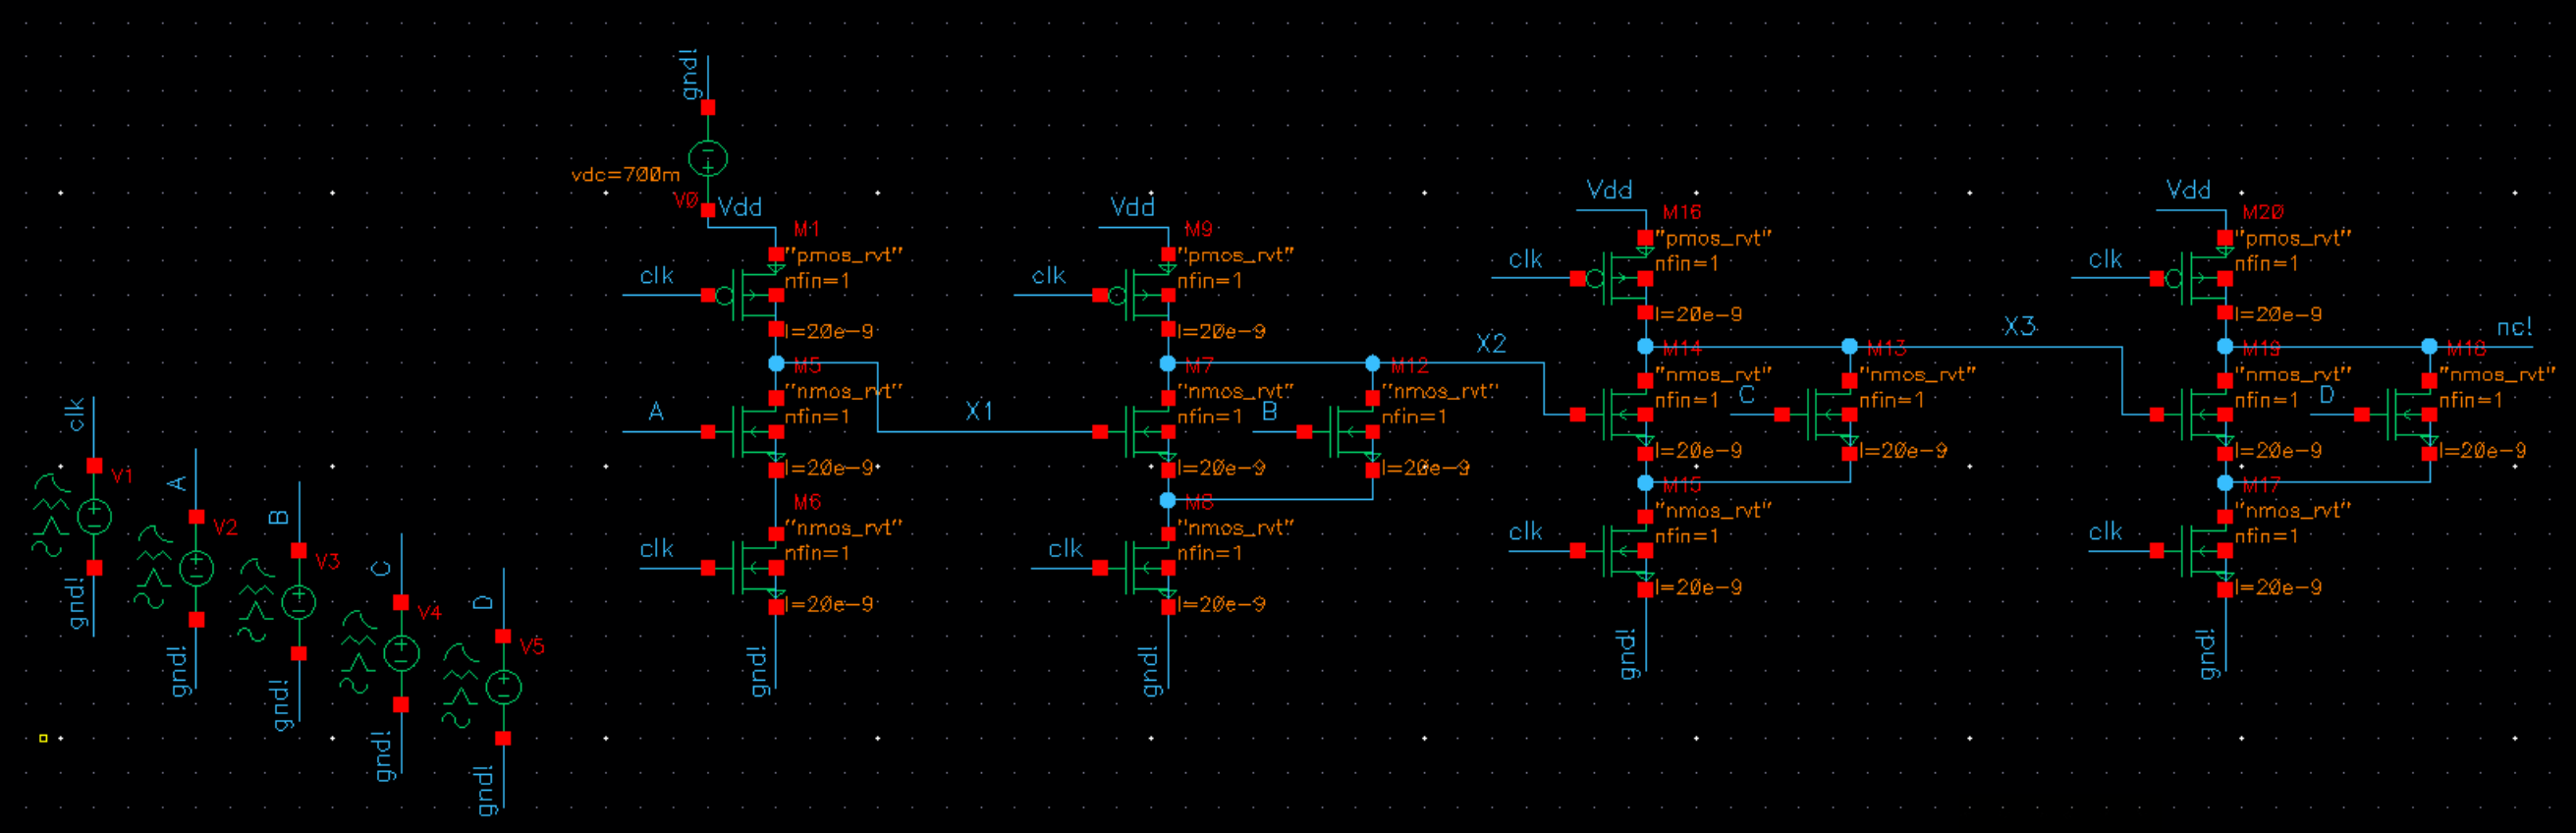
\includegraphics[width=0.45\linewidth, height=0.20\textheight, keepaspectratio]{Images/sch_p3.png}\hfill
  \\[\smallskipamount]
  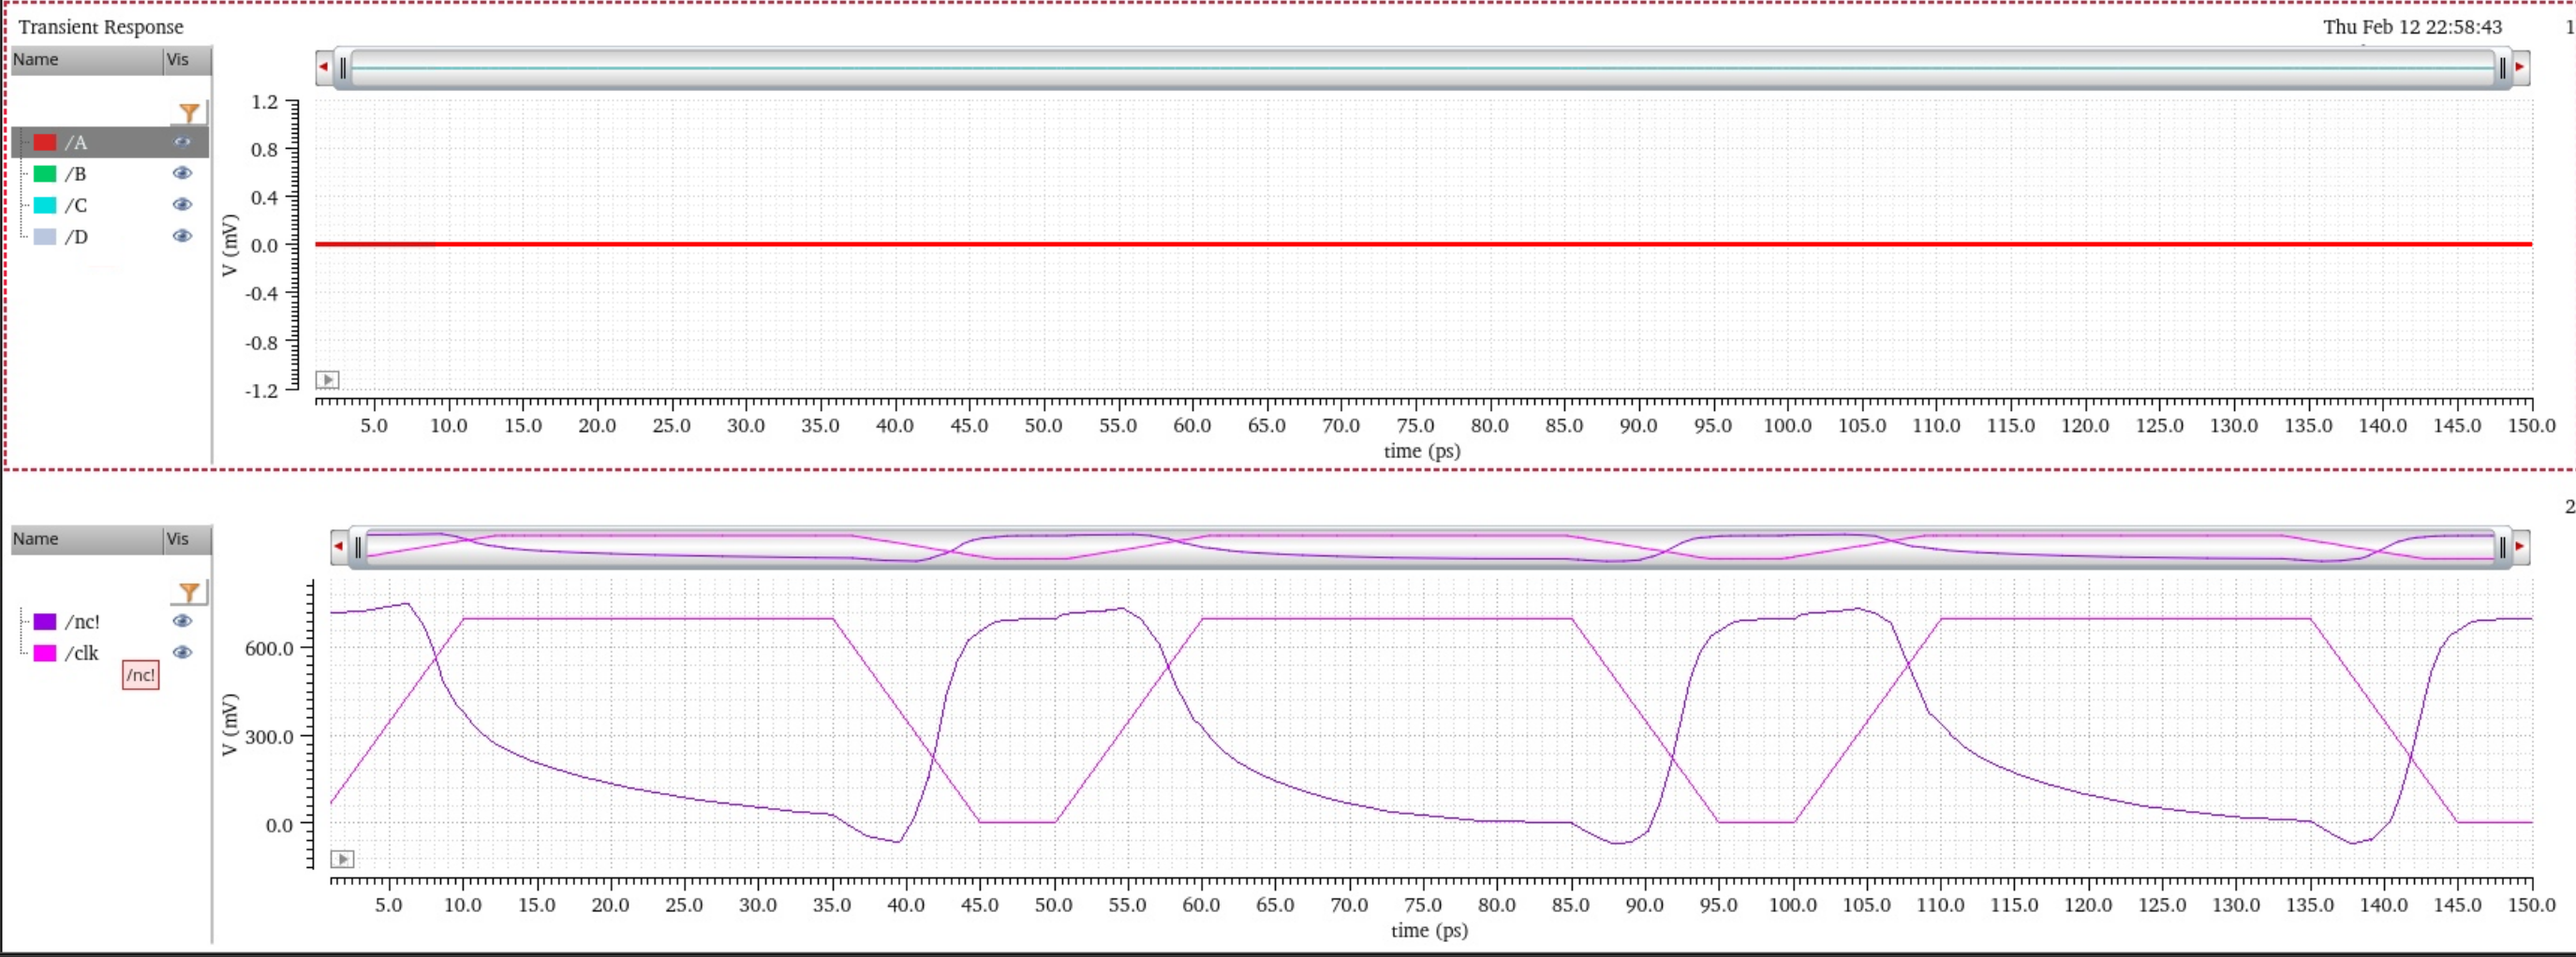
\includegraphics[width=0.45\linewidth, height=0.20\textheight, keepaspectratio]{Images/output_p3_0000_2.png}\hfill
  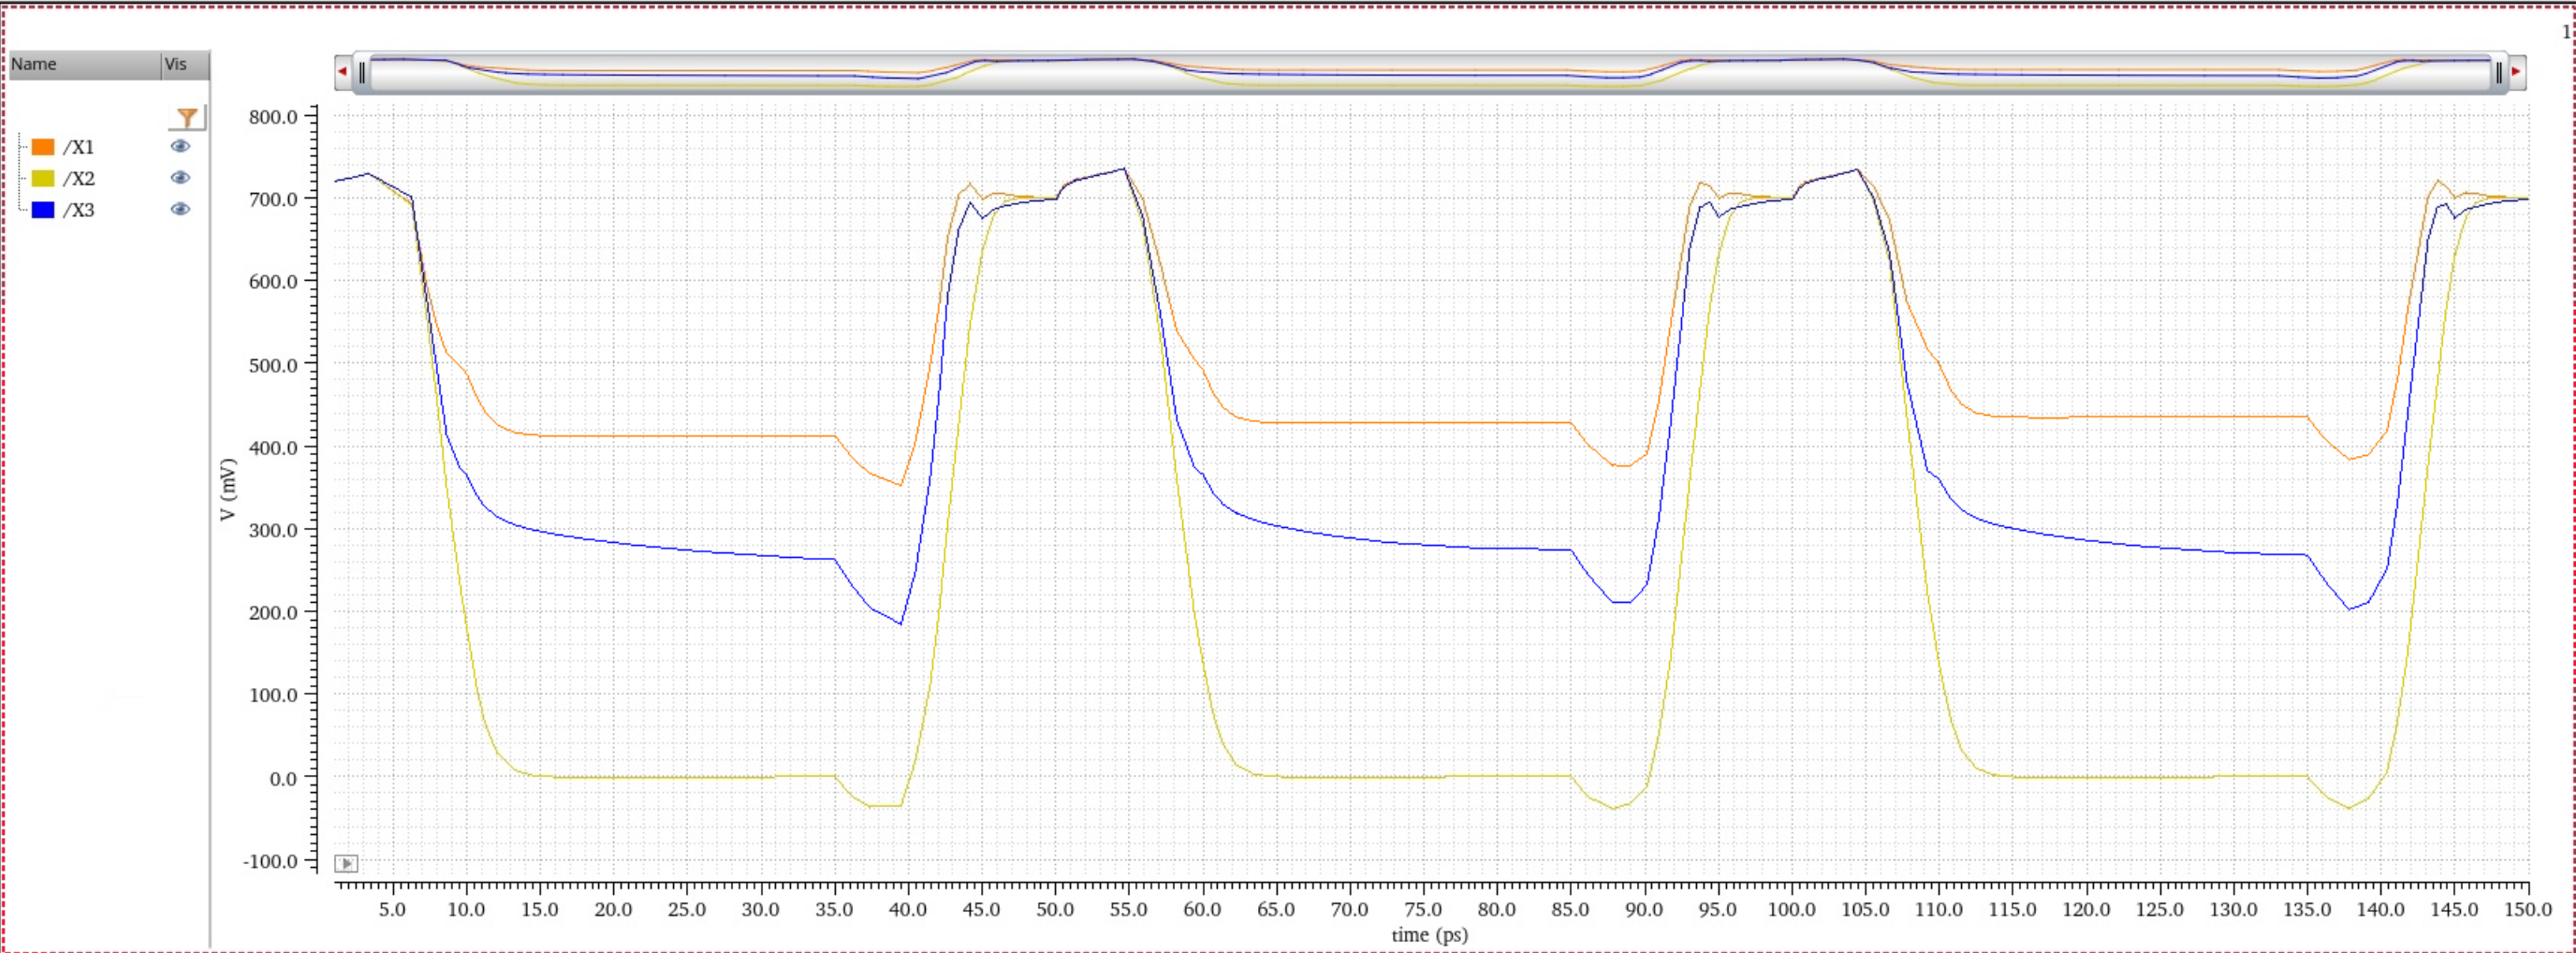
\includegraphics[width=0.54\linewidth, height=0.20\textheight, keepaspectratio]{Images/output_p3_0000_2_int.png}
  \\[\smallskipamount]
  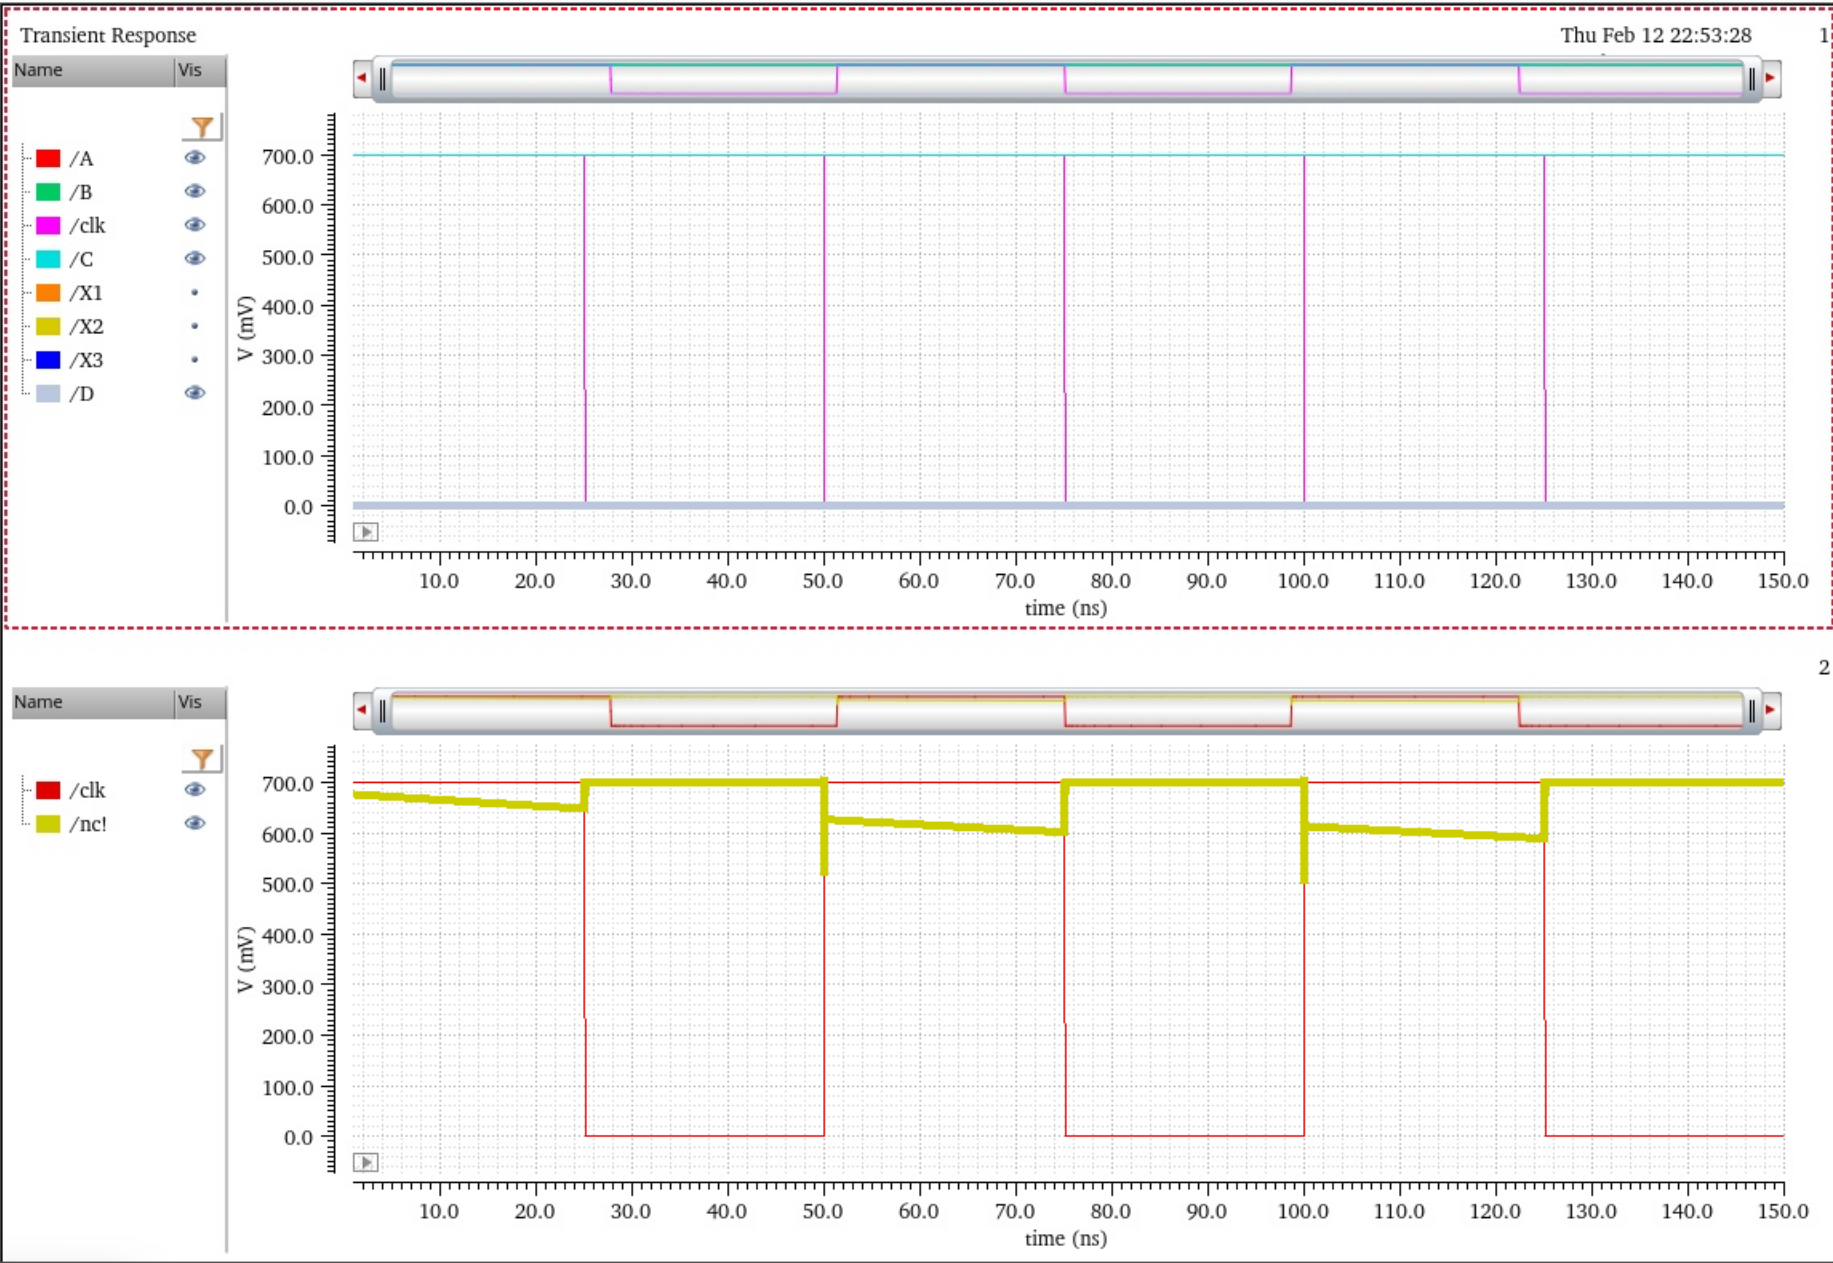
\includegraphics[width=0.45\linewidth, height=0.20\textheight, keepaspectratio]{Images/output_p3_1110_2.png}\hfill
  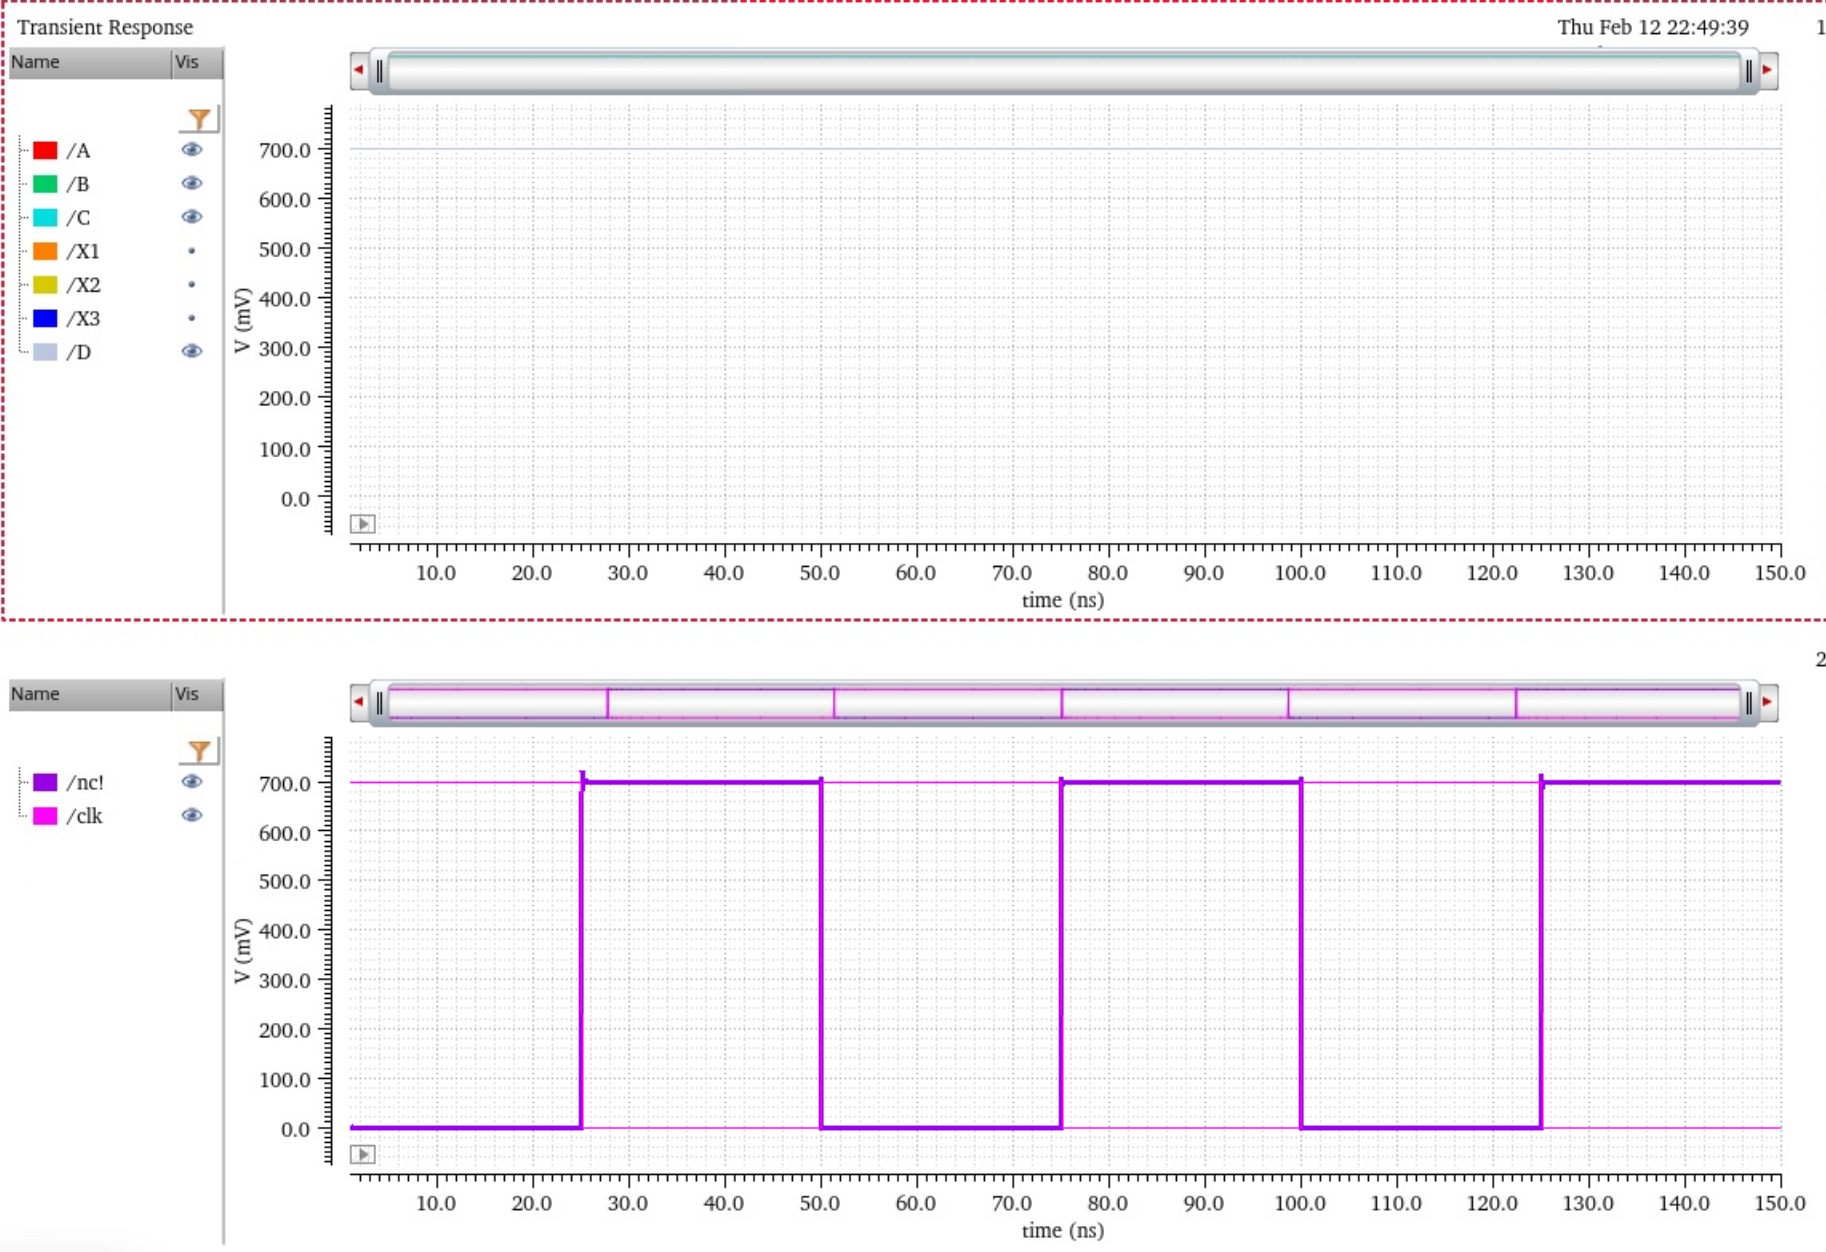
\includegraphics[width=0.45\linewidth, height=0.20\textheight, keepaspectratio]{Images/output_p3_1111_2.png}\hfill
  \caption{Problem 3. Schematic (Top row). Input 0000 with intermediate values (second row). Input 1110 (left) and 1111 (right) (third row).}
  \label{fid:output_p3_1}
  \parbox{\linewidth}{Similar behavior happens to the Function F=A+B+C. There is a logic error when all values are 0. And there is a charge and dischare every clk cycle.}
\end{figure}



\begin{figure}[h]
  \centering
  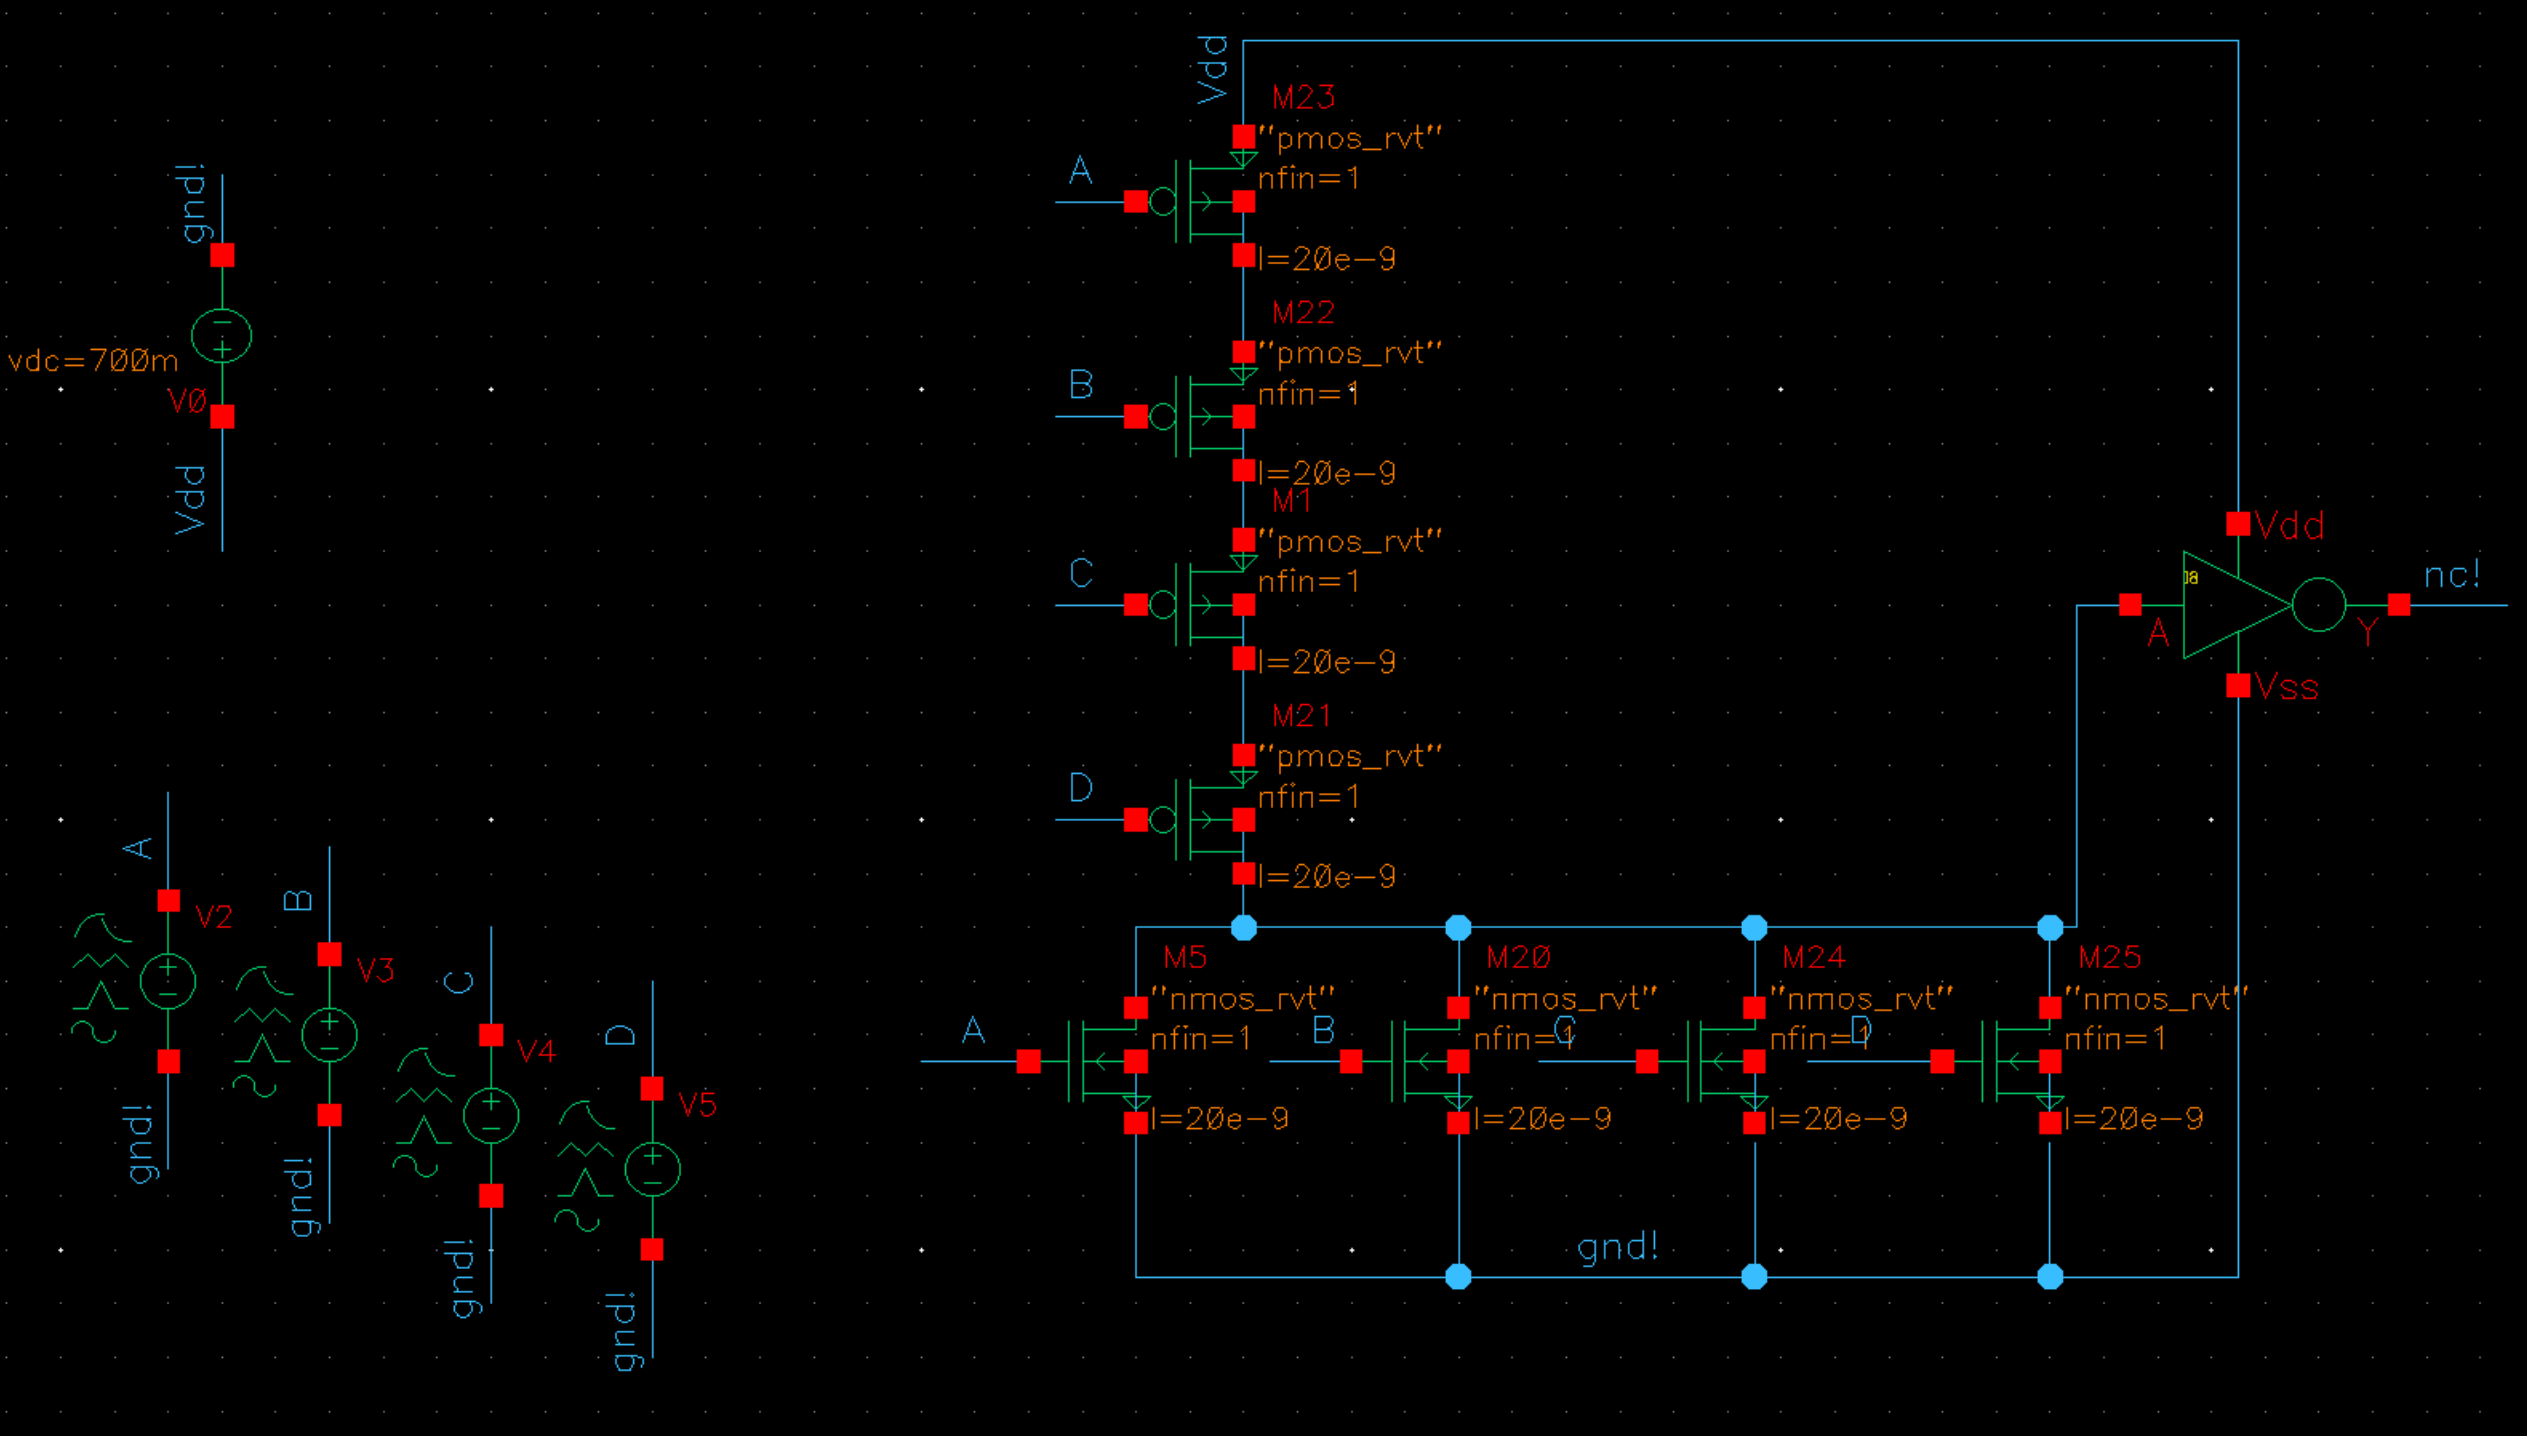
\includegraphics[width=0.45\linewidth, height=0.20\textheight, keepaspectratio]{Images/sch_p3_cmos.png}\hfill
  \\[\smallskipamount]
  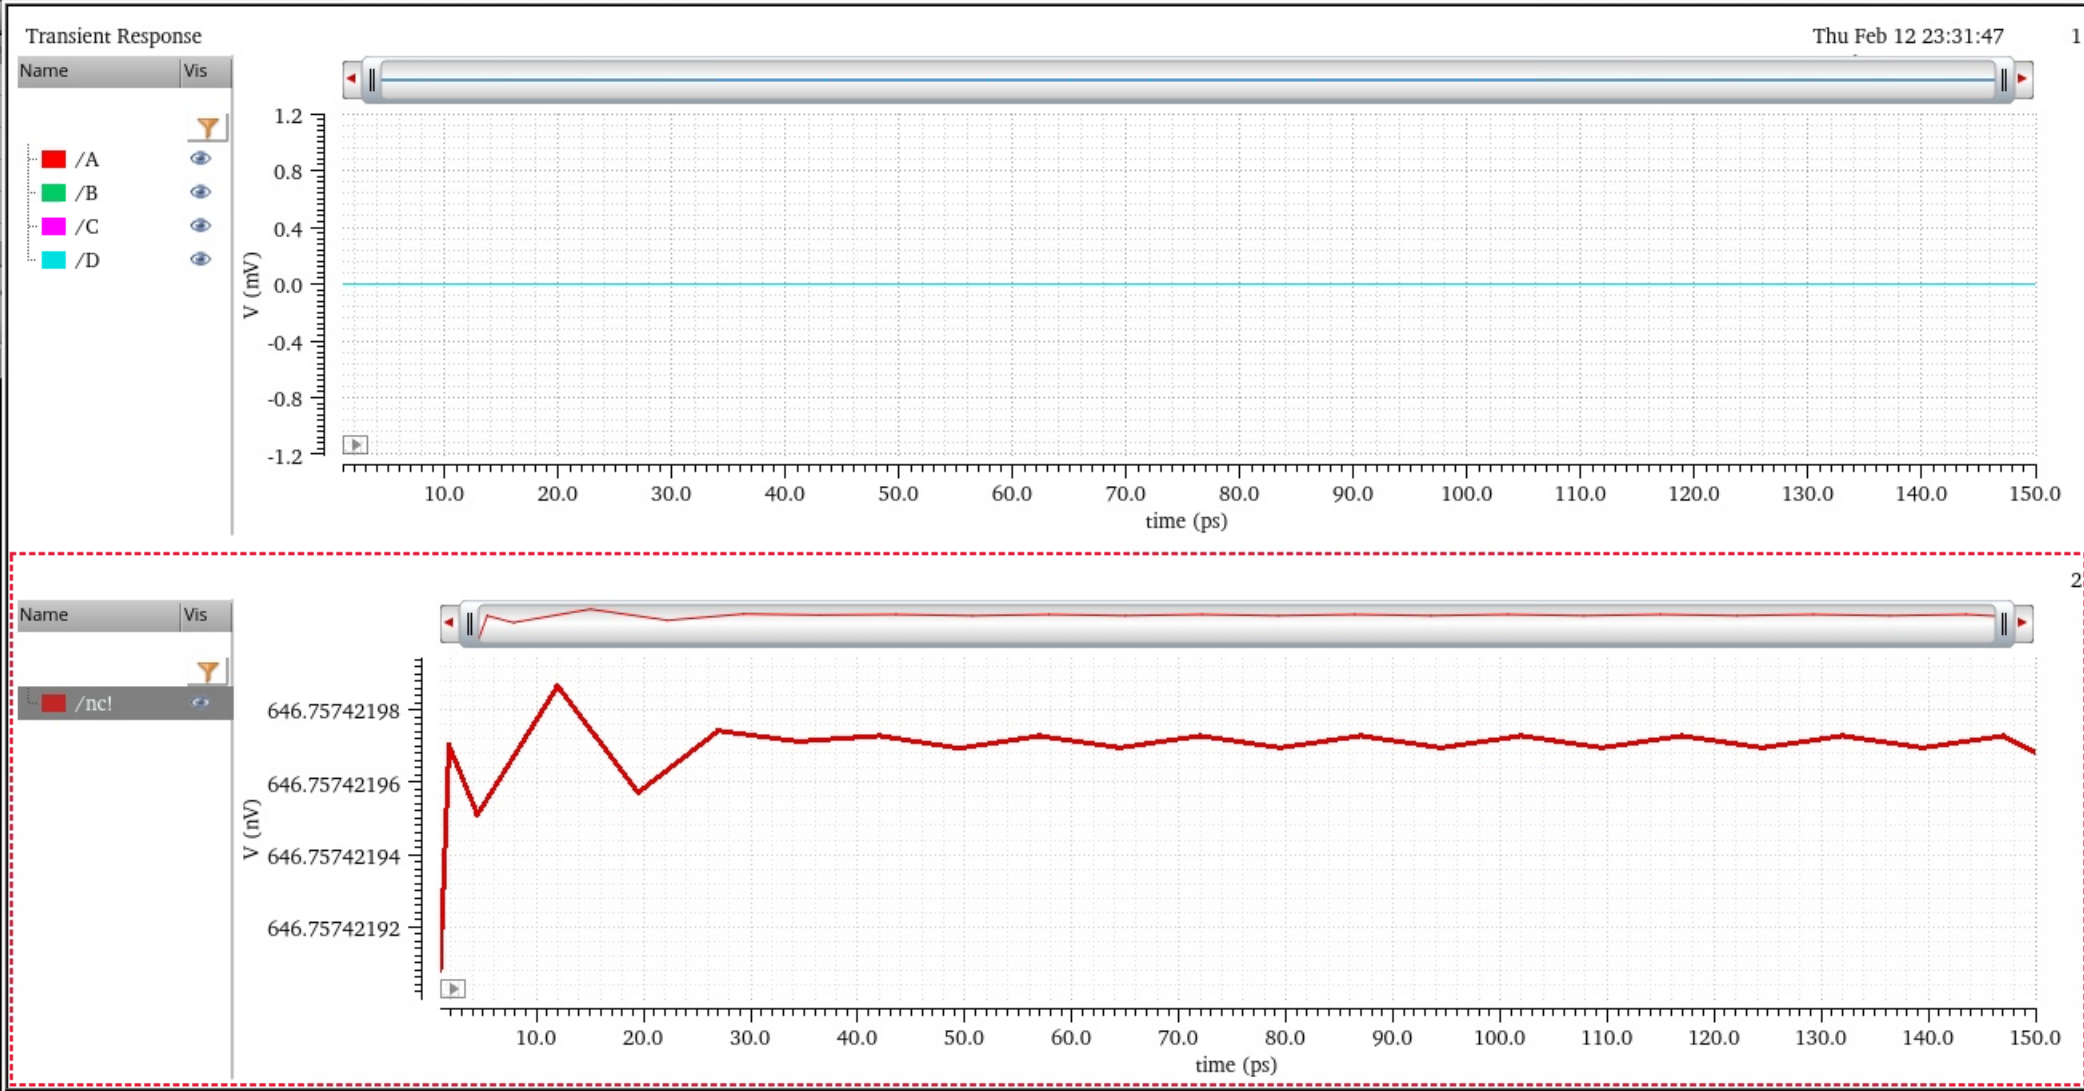
\includegraphics[width=0.45\linewidth, height=0.20\textheight, keepaspectratio]{Images/output_0000_p3_cmos.png}\hfill
  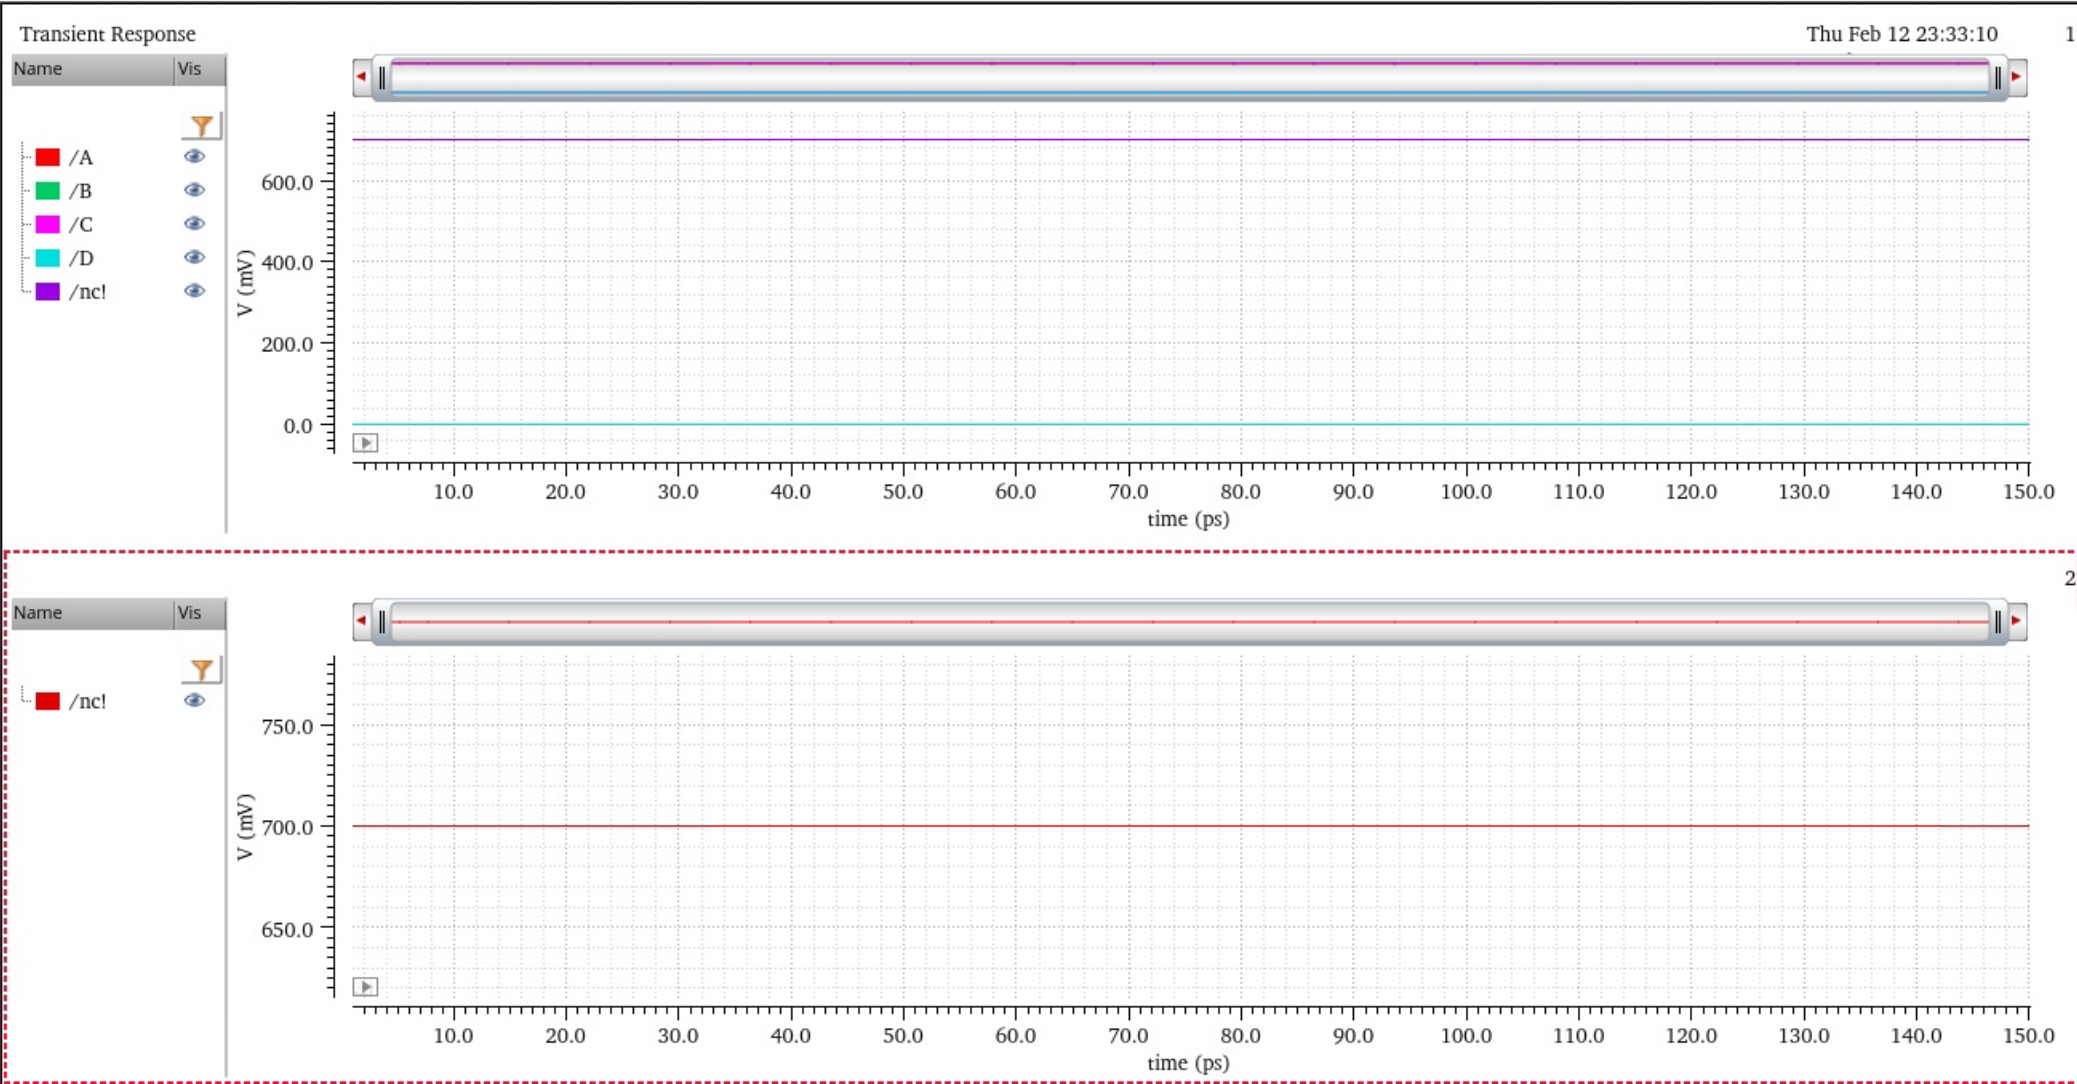
\includegraphics[width=0.54\linewidth, height=0.20\textheight, keepaspectratio]{Images/output_1000_p3_cmos.png}
  \caption{Problem 3. Schematic (Top row). Input 0000 (left) and 1000(right) (Bottom row).}
  \label{fid:output_p3_1}
  \parbox{\linewidth}{The logic is correct. And there is no charging discharging with every clk cycle. The same argument applies to the function F=A+B+C.}
\end{figure}


\clearpage

\section*{Problem 4}

\begin{figure}[h]
  \centering
  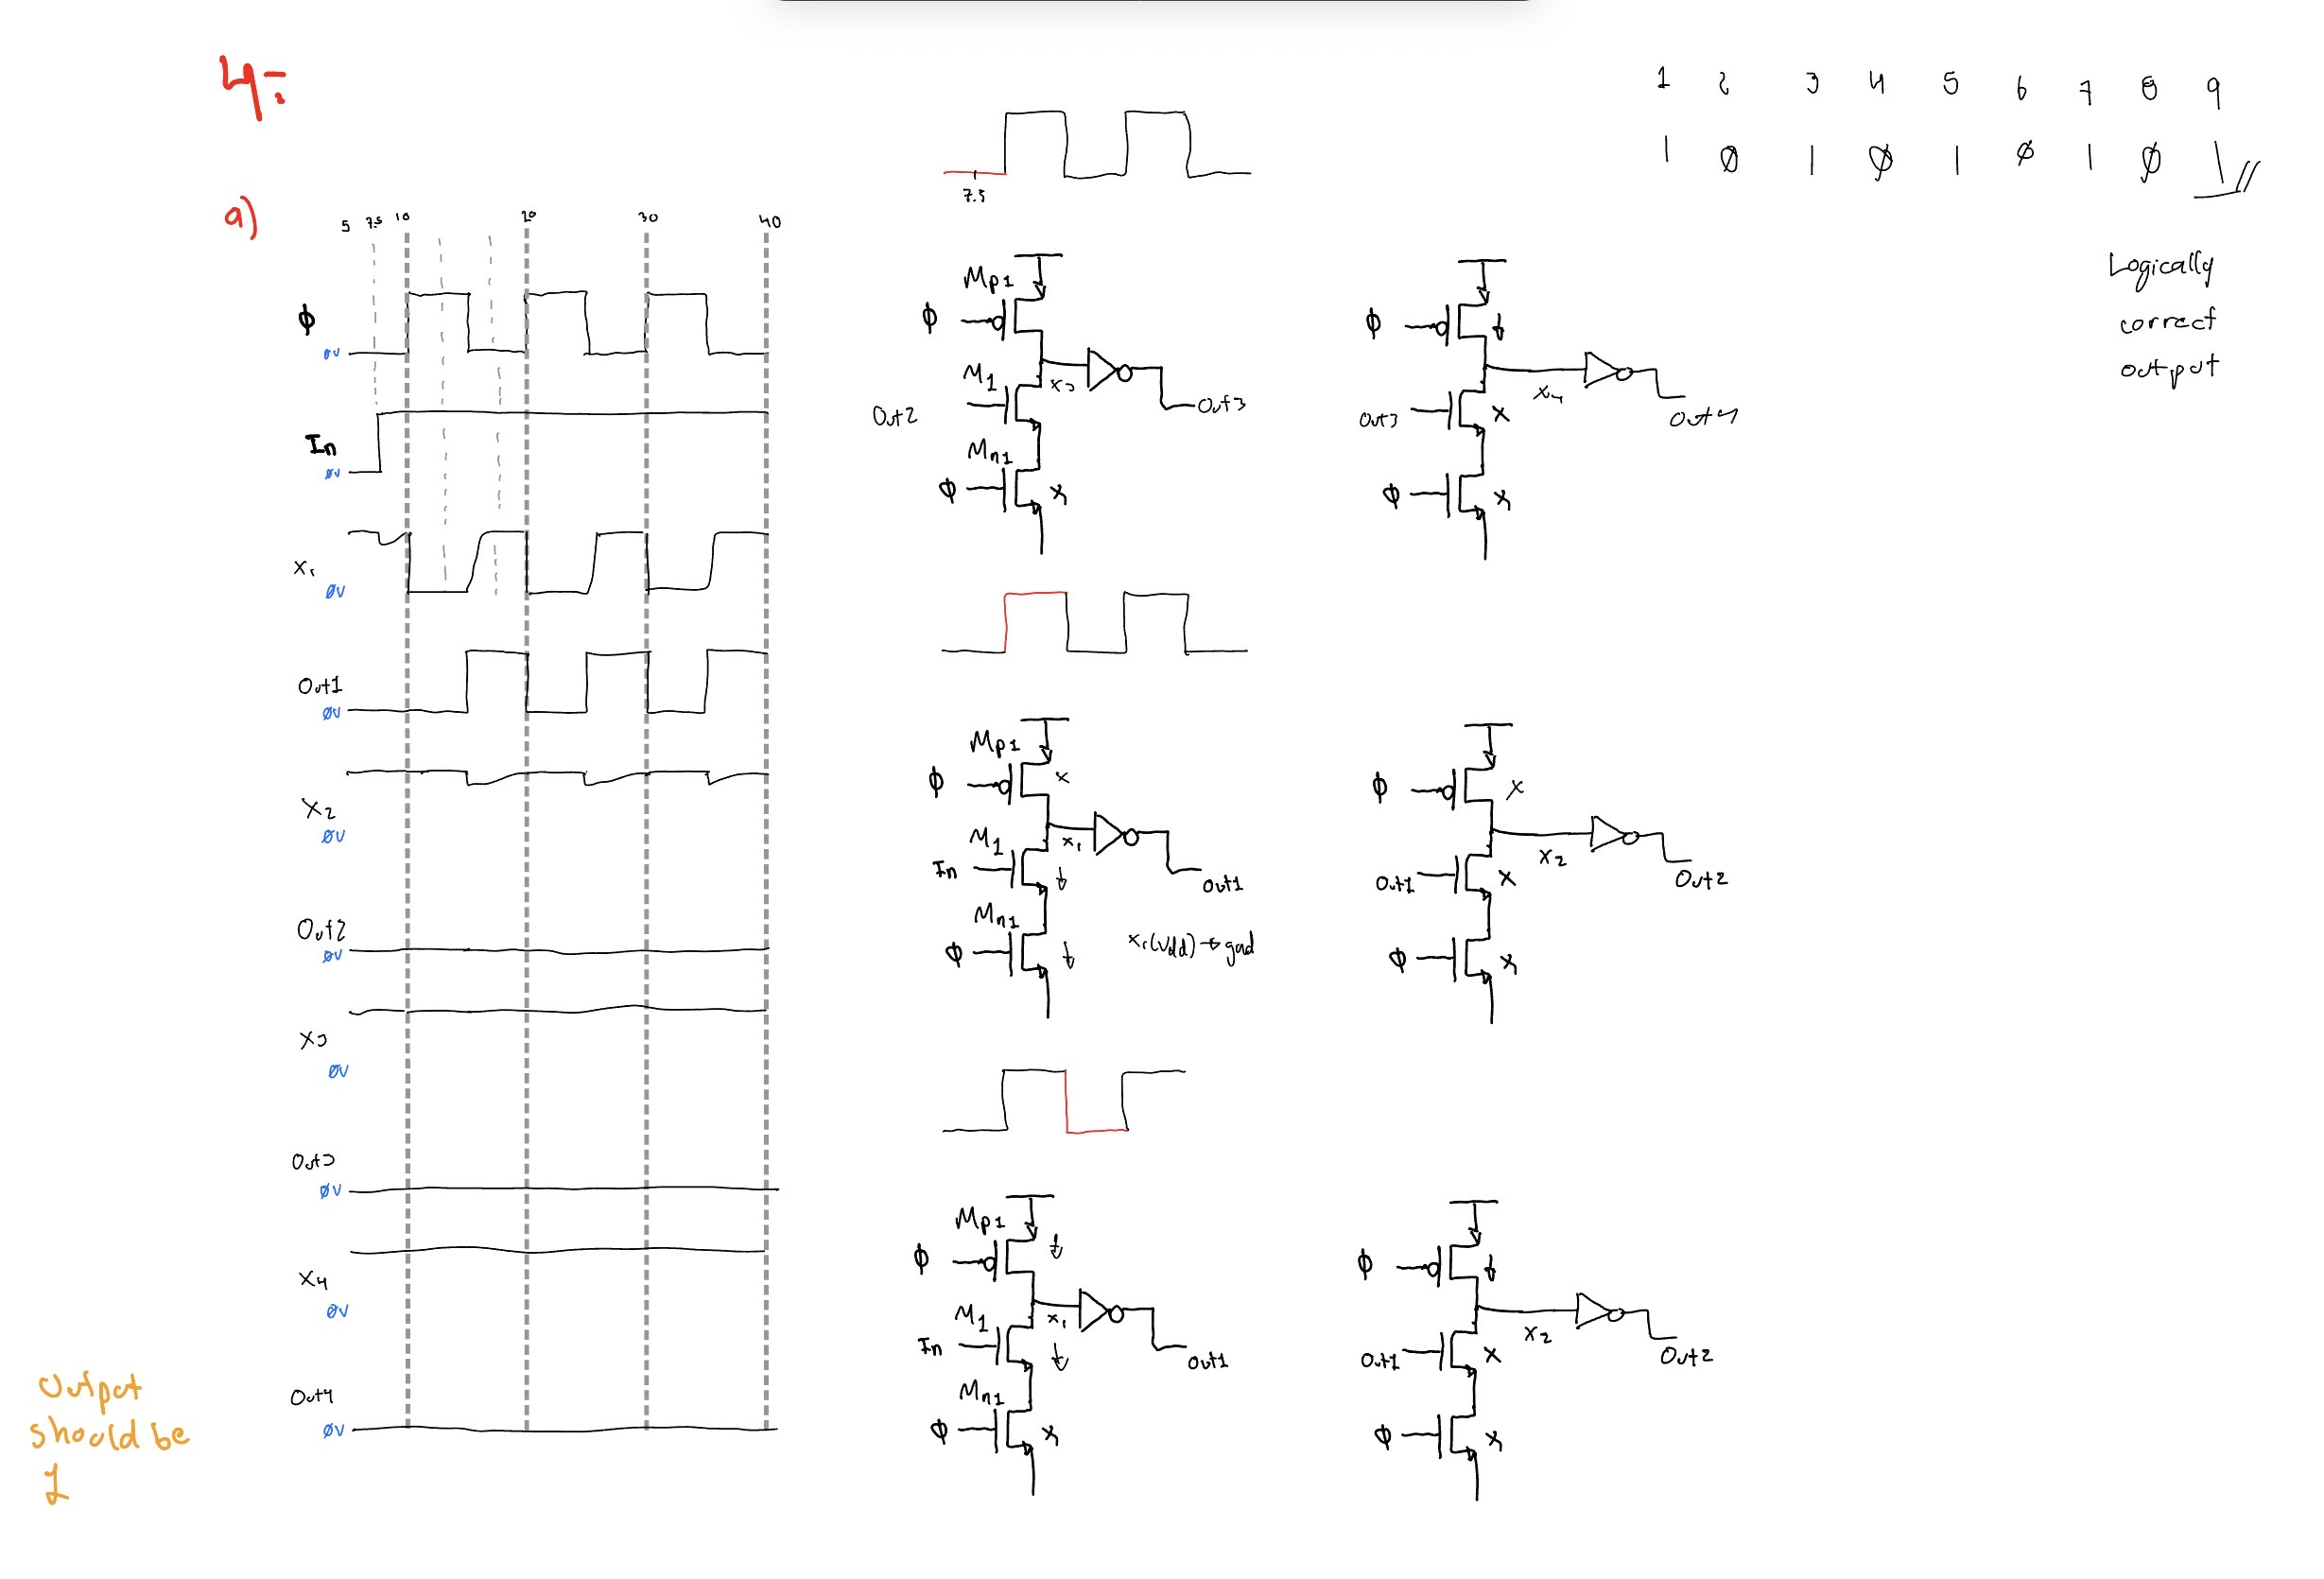
\includegraphics[width=0.45\linewidth, height=0.20\textheight, keepaspectratio]{Images/IMG_1142.jpg}\hfill
  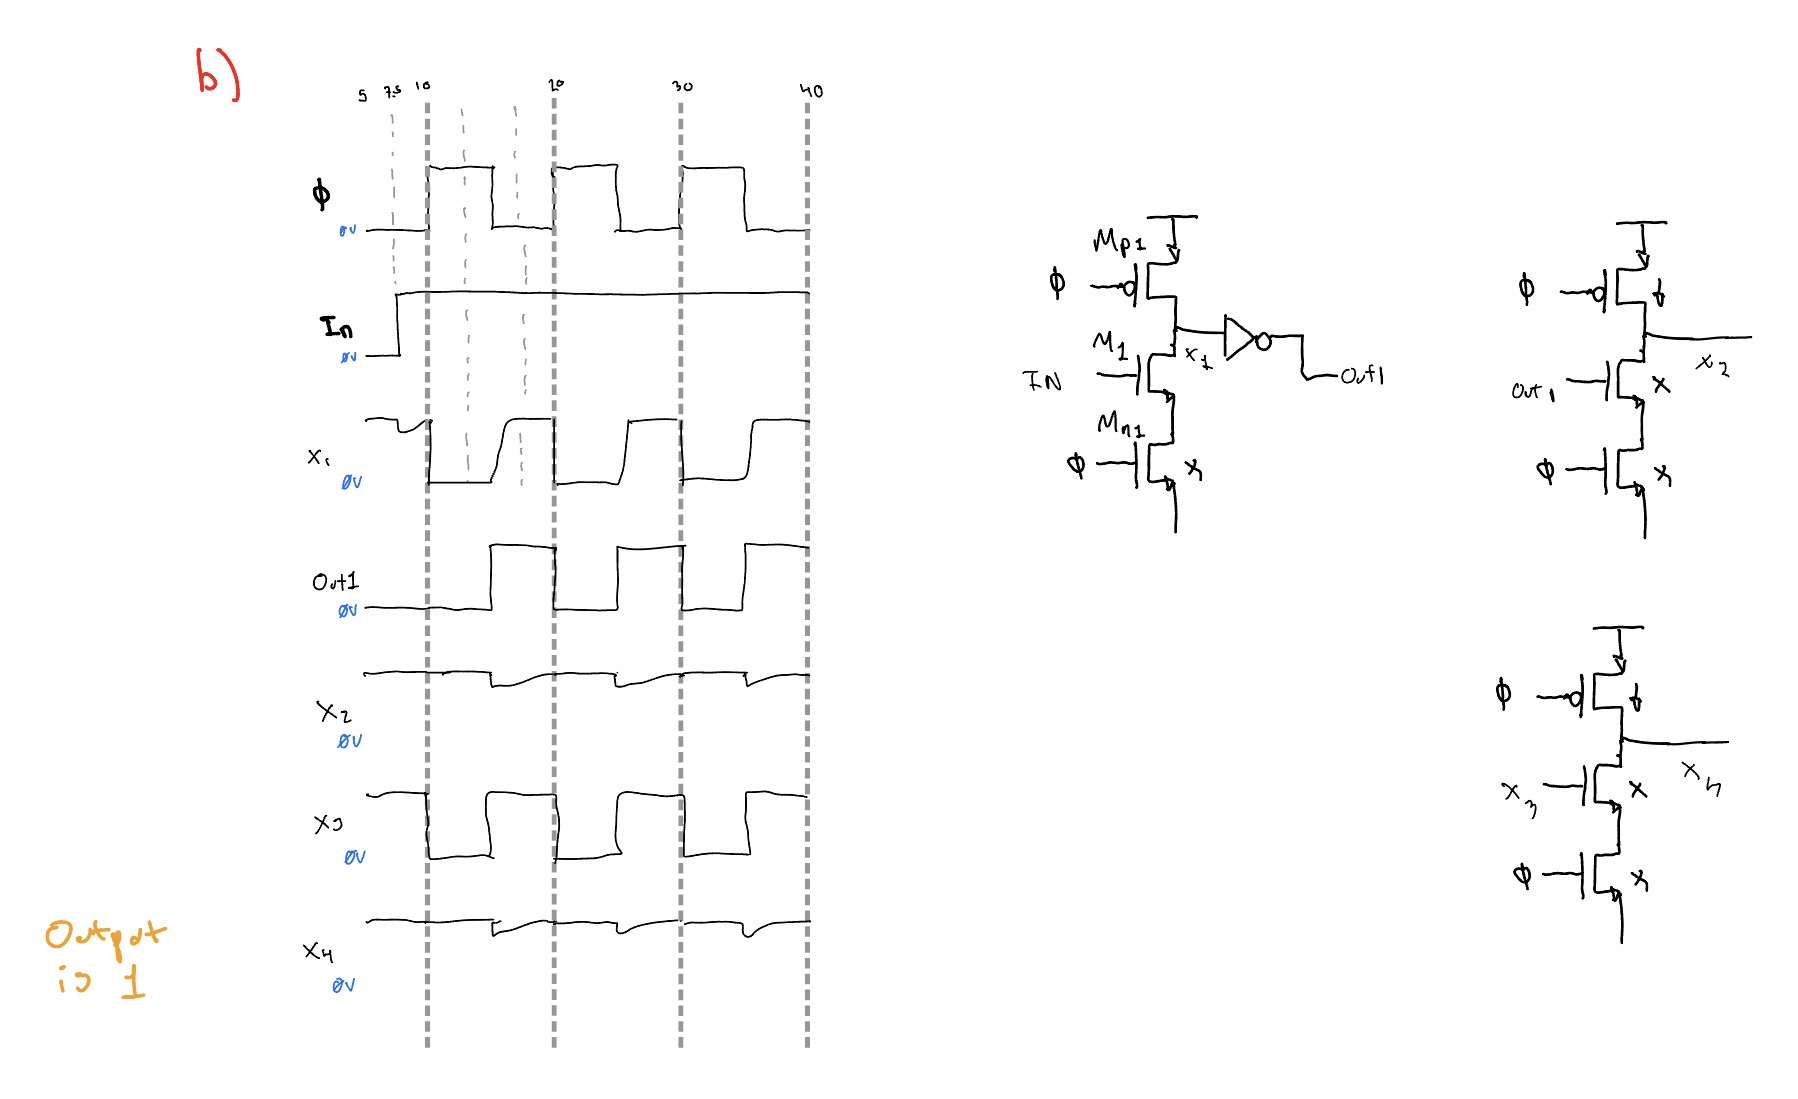
\includegraphics[width=0.45\linewidth, height=0.20\textheight, keepaspectratio]{Images/IMG_1143.jpg}\hfill
  \\[\smallskipamount]
  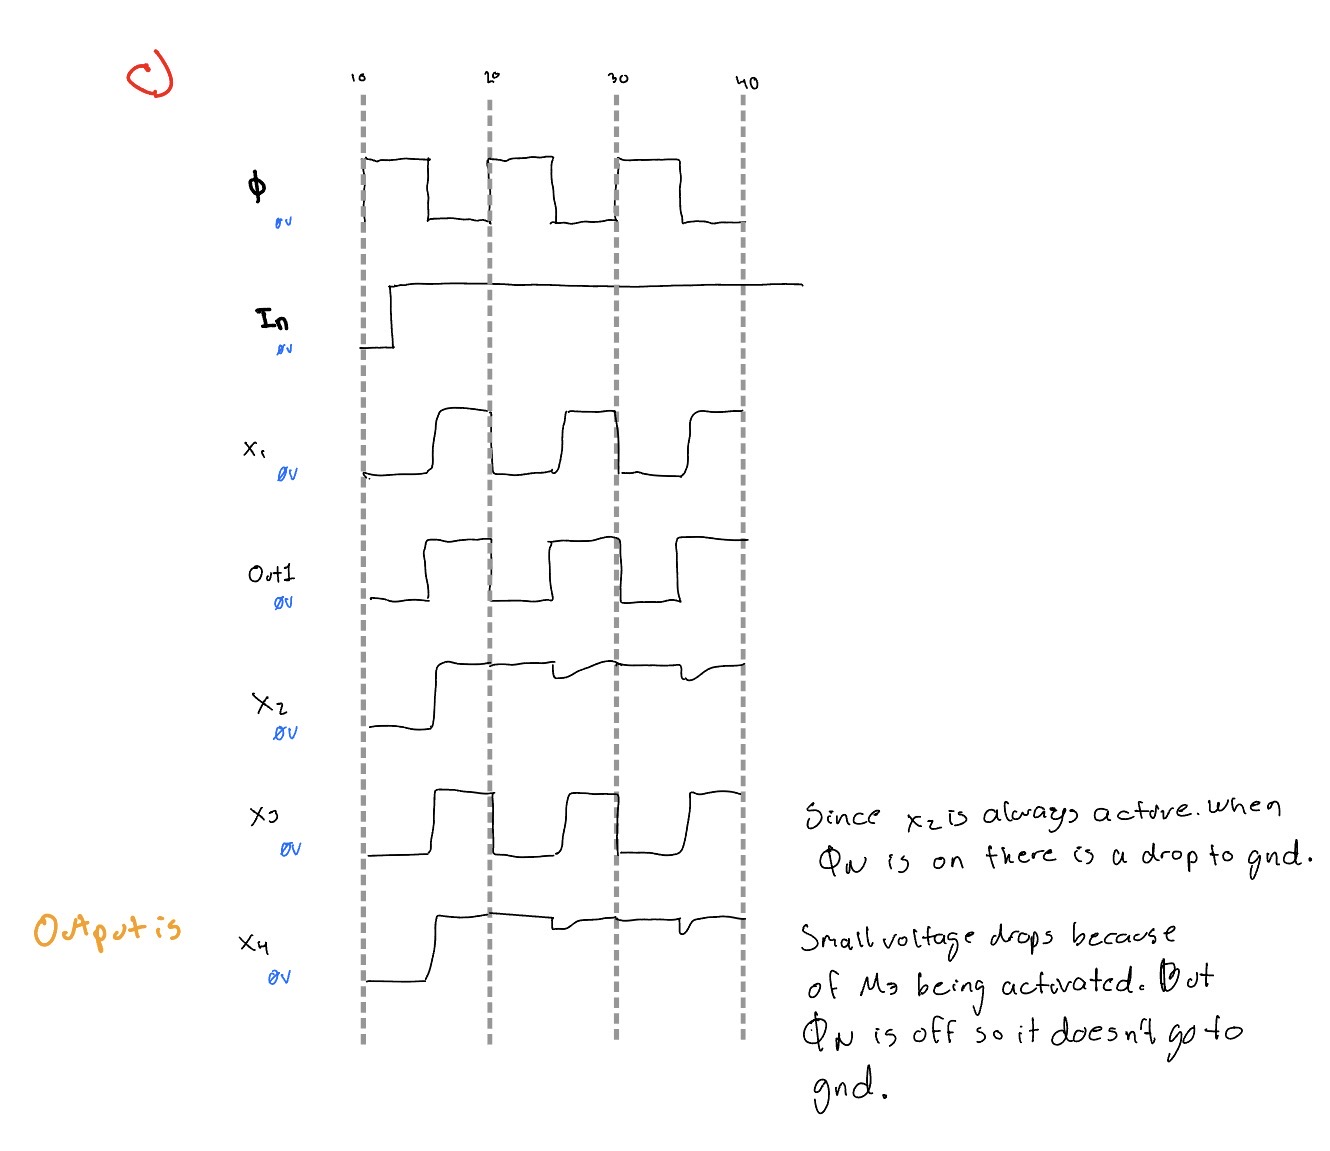
\includegraphics[width=0.45\linewidth, height=0.20\textheight, keepaspectratio]{Images/IMG_1144.jpg}\hfill
  \caption{Problem 4. Sketches of waveforms.}
  \label{fig:sketches_p4}
\end{figure}

\begin{figure}[h]
  \centering
  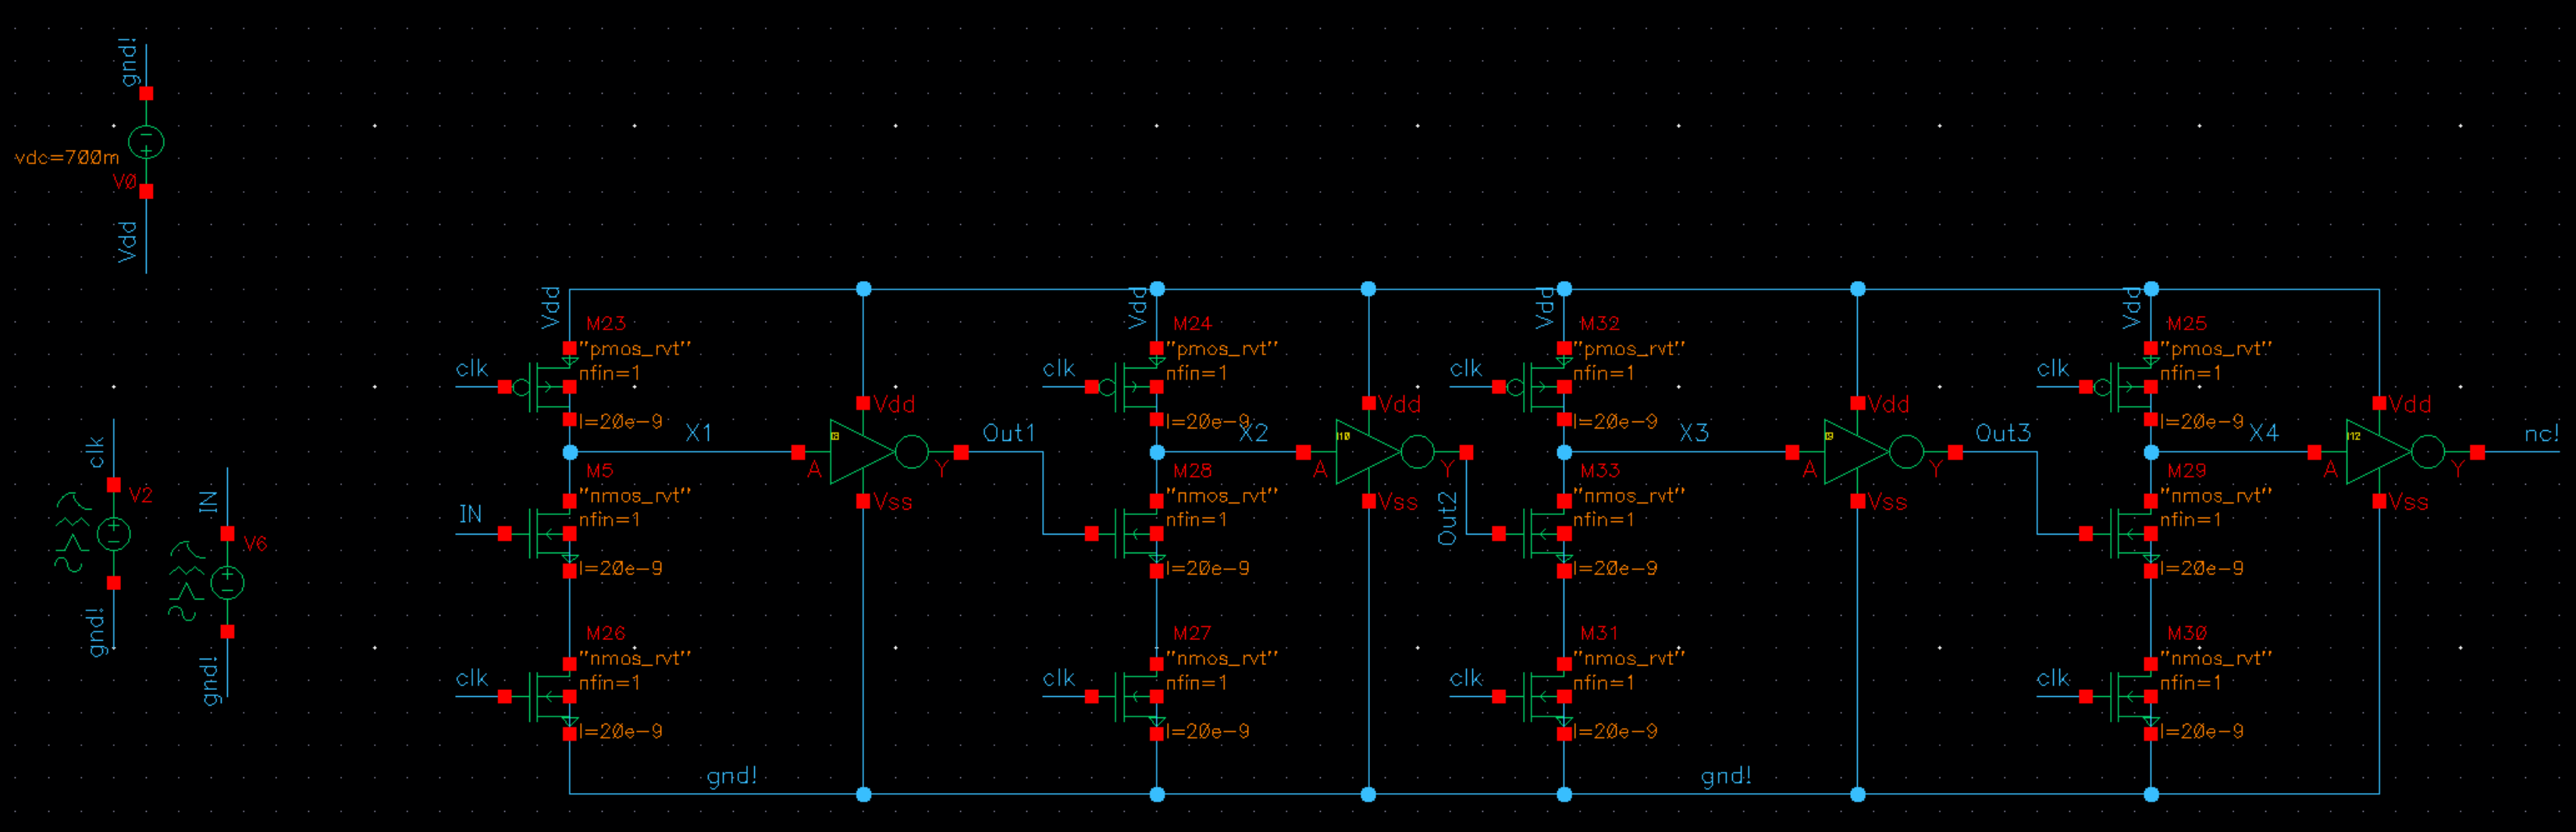
\includegraphics[width=0.45\linewidth, height=0.20\textheight, keepaspectratio]{Images/sch_p4_1.png}\hfill
  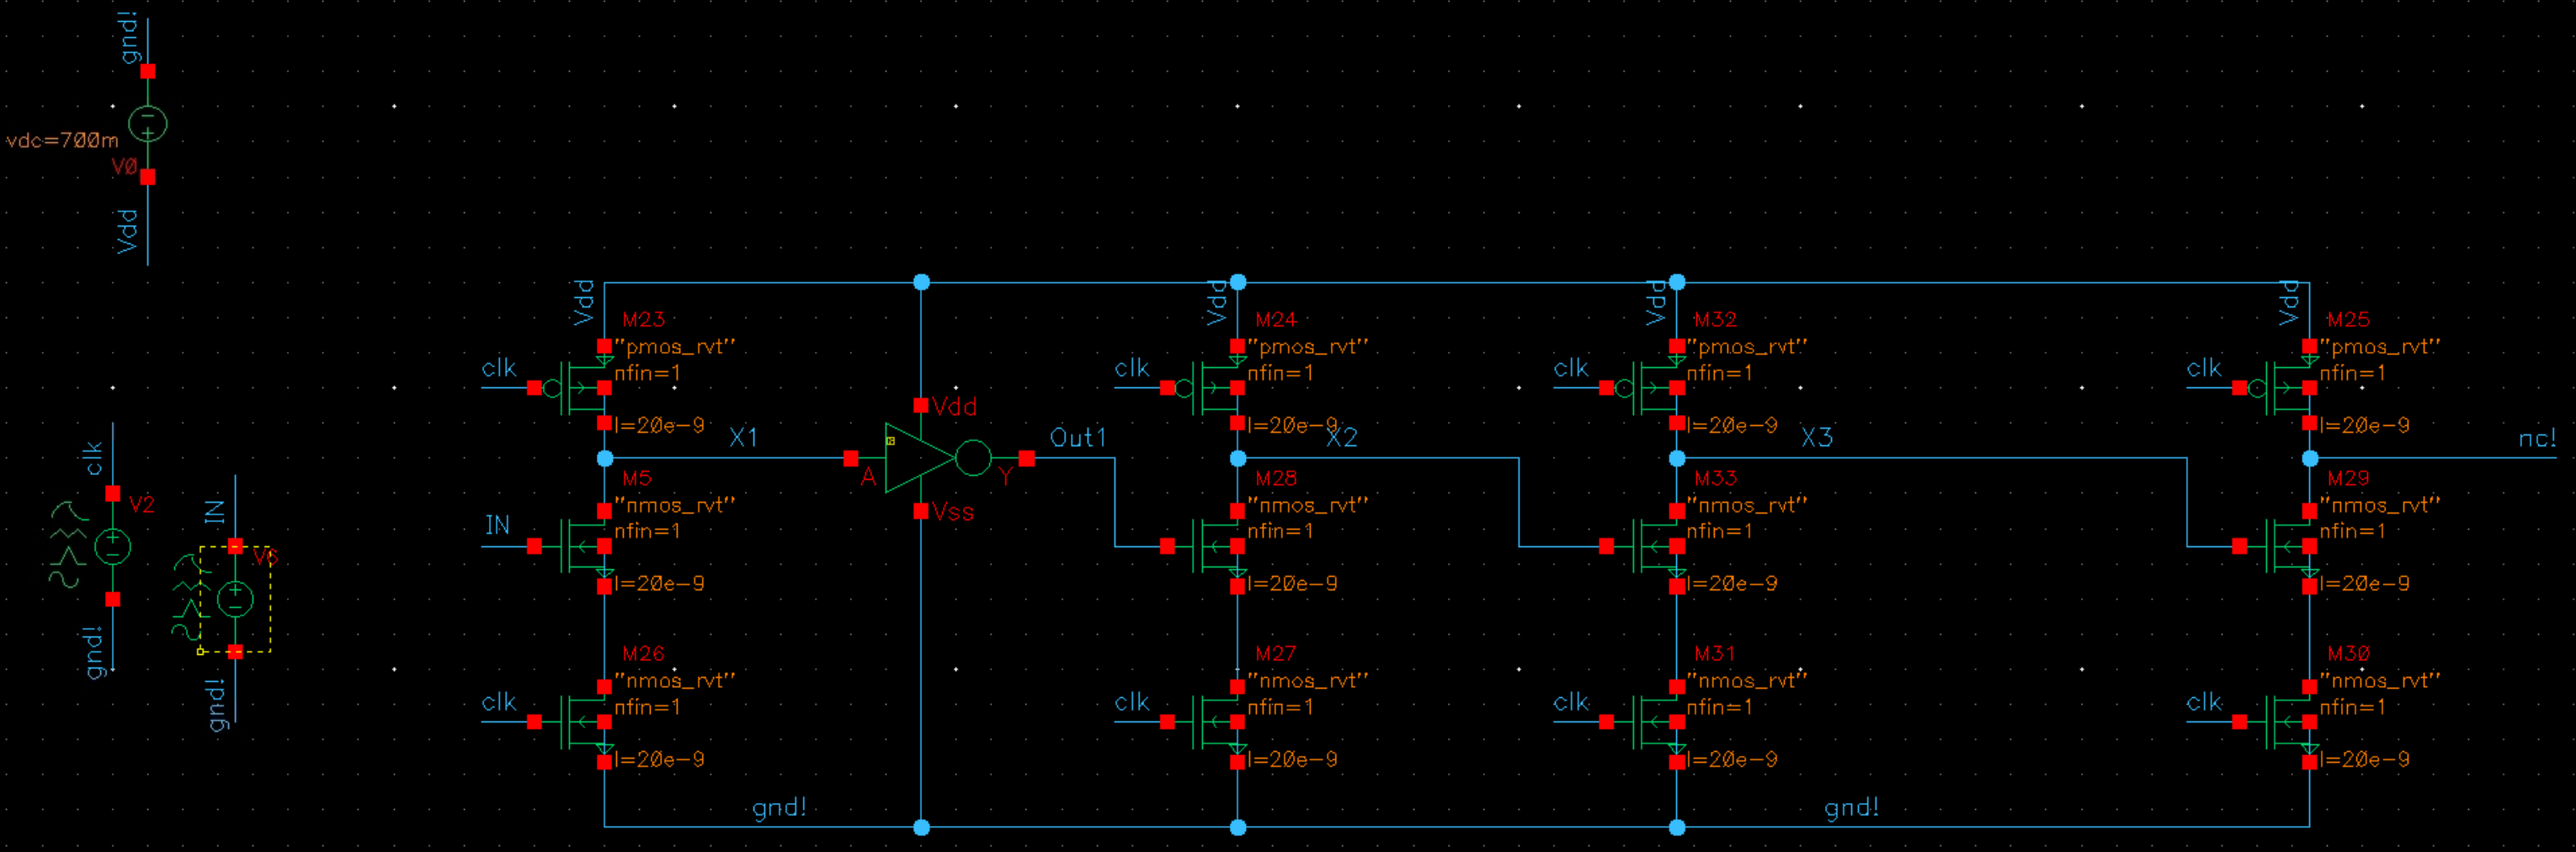
\includegraphics[width=0.45\linewidth, height=0.20\textheight, keepaspectratio]{Images/sch_p4_2.png}\hfill
  \caption{Problem 4. Schematic with switches (left). Schematic no switched (right).}
  \label{fig:sch_p4}
\end{figure}

\begin{figure}[h]
  \centering
  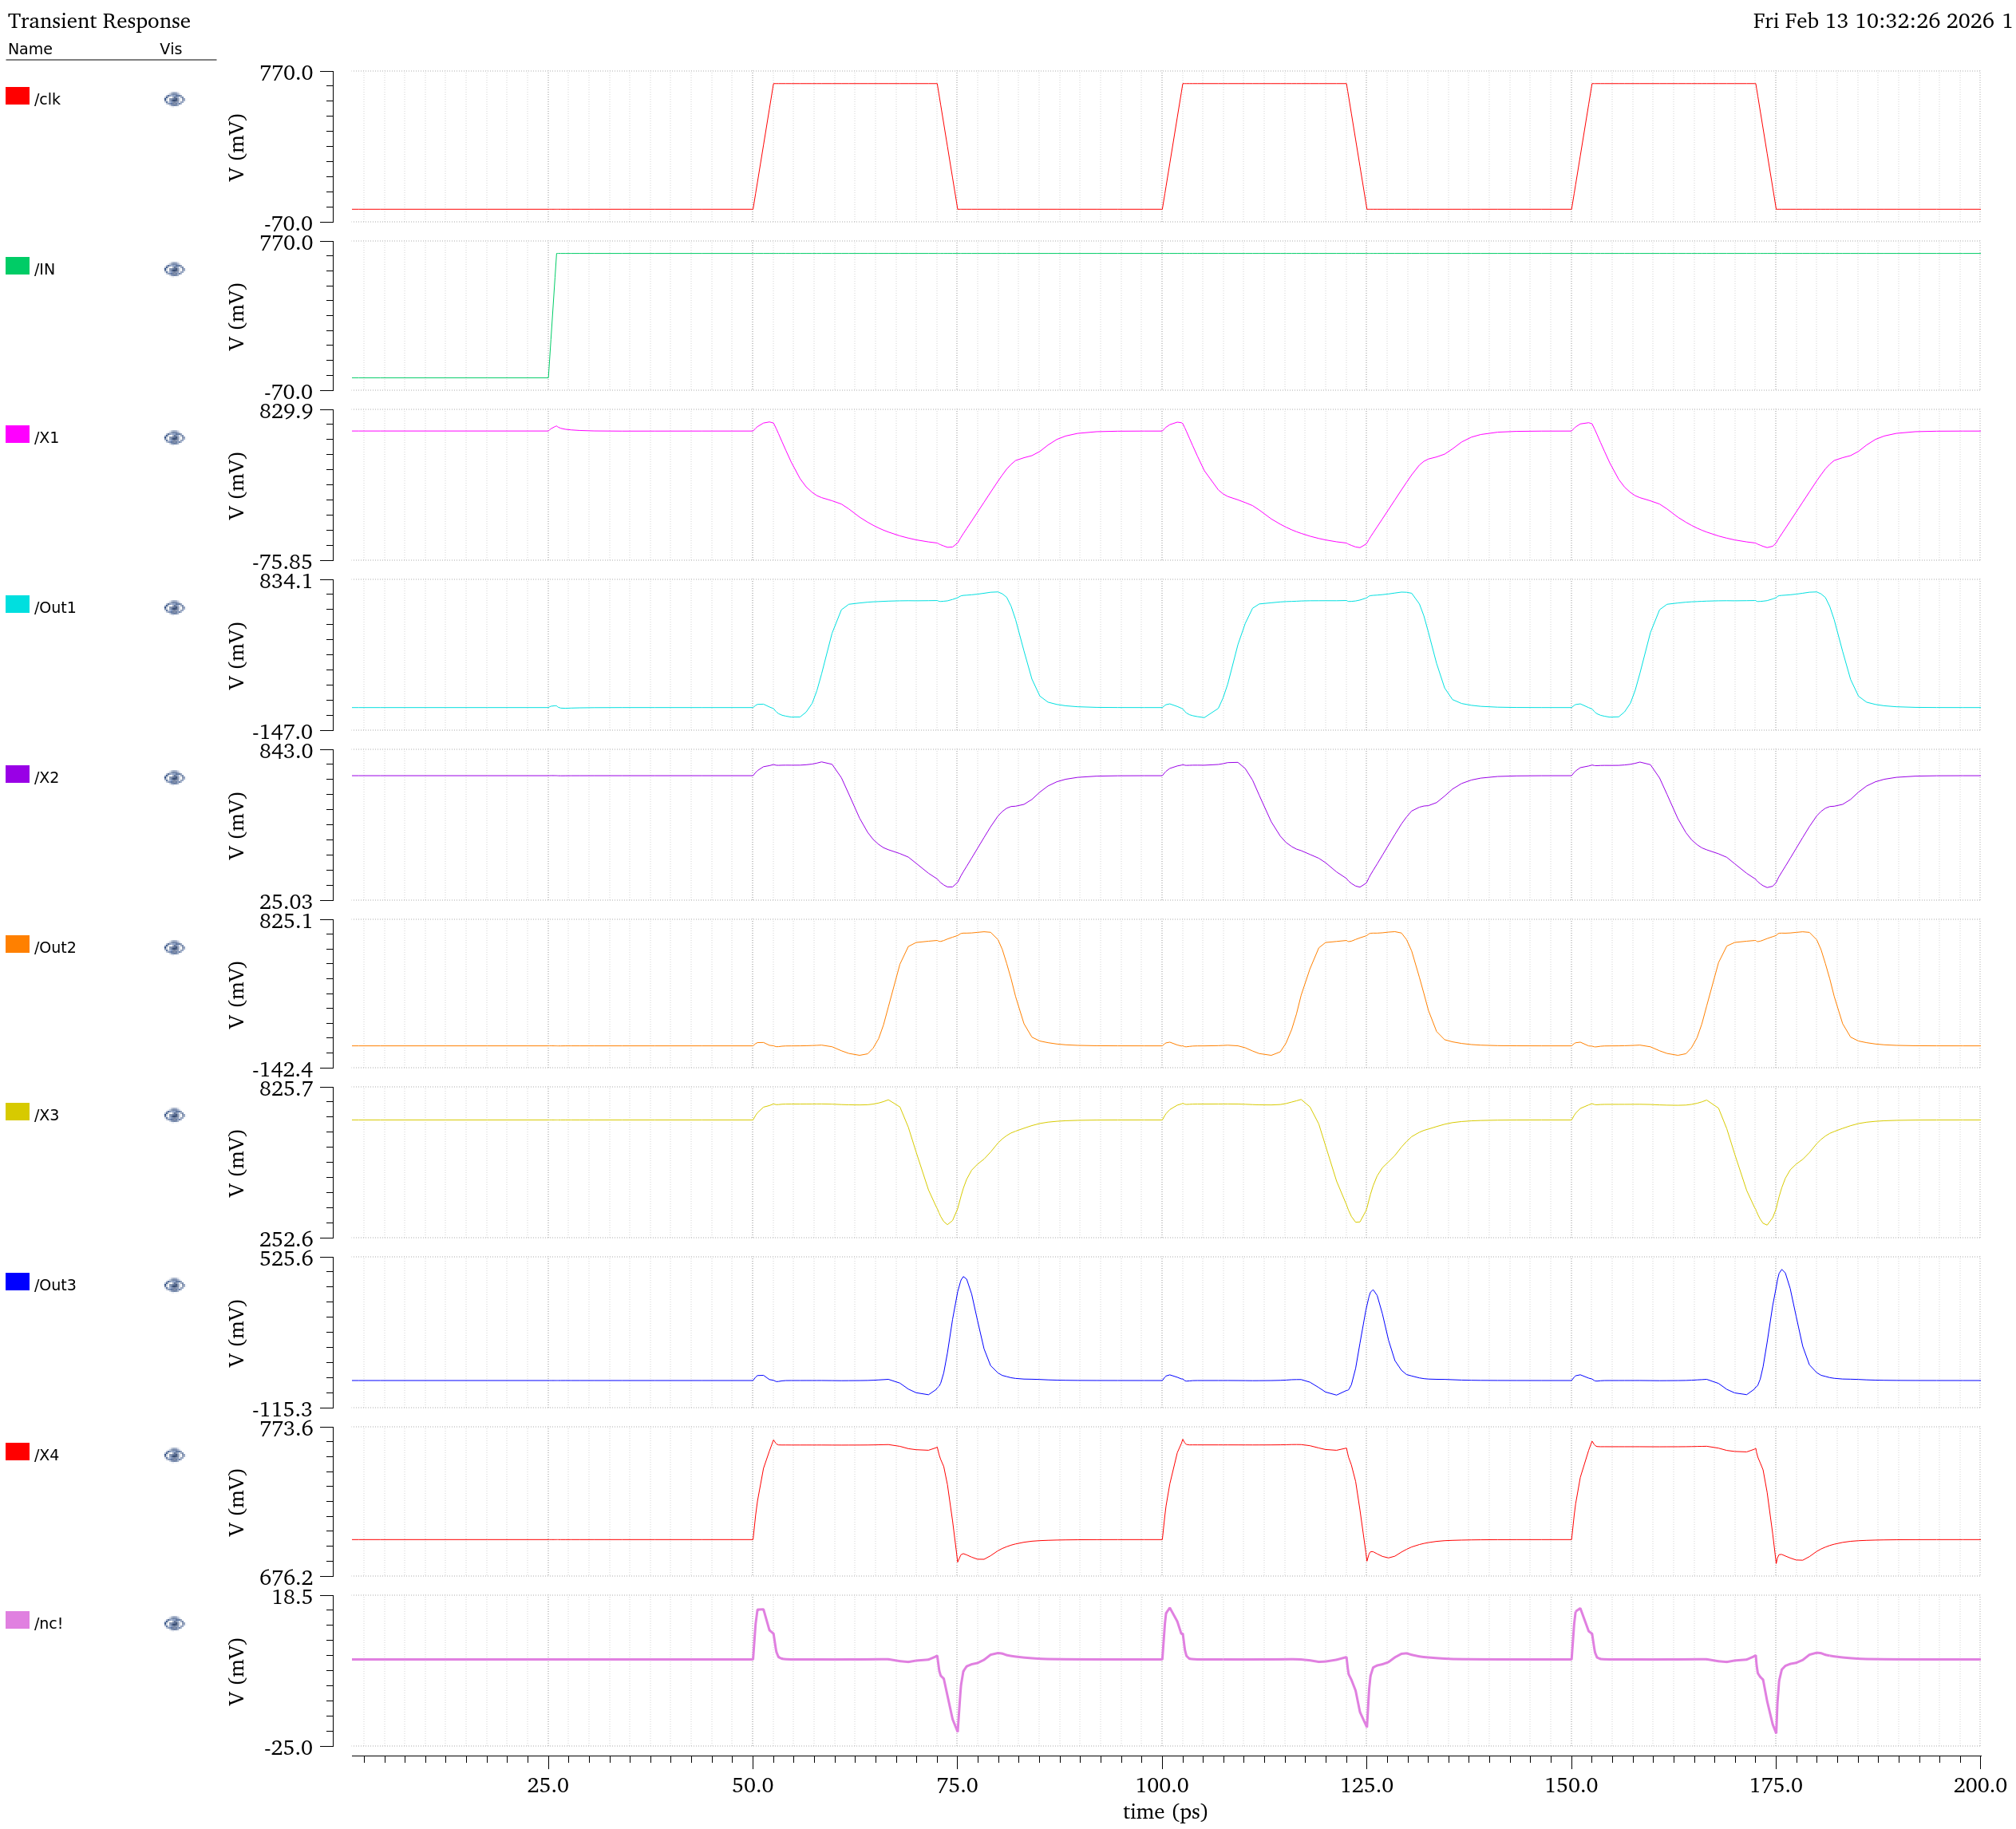
\includegraphics[width=0.49\linewidth, height=0.50\textheight, keepaspectratio]{Images/hw1_p4_vlsi_ii_1.png}\hfill
  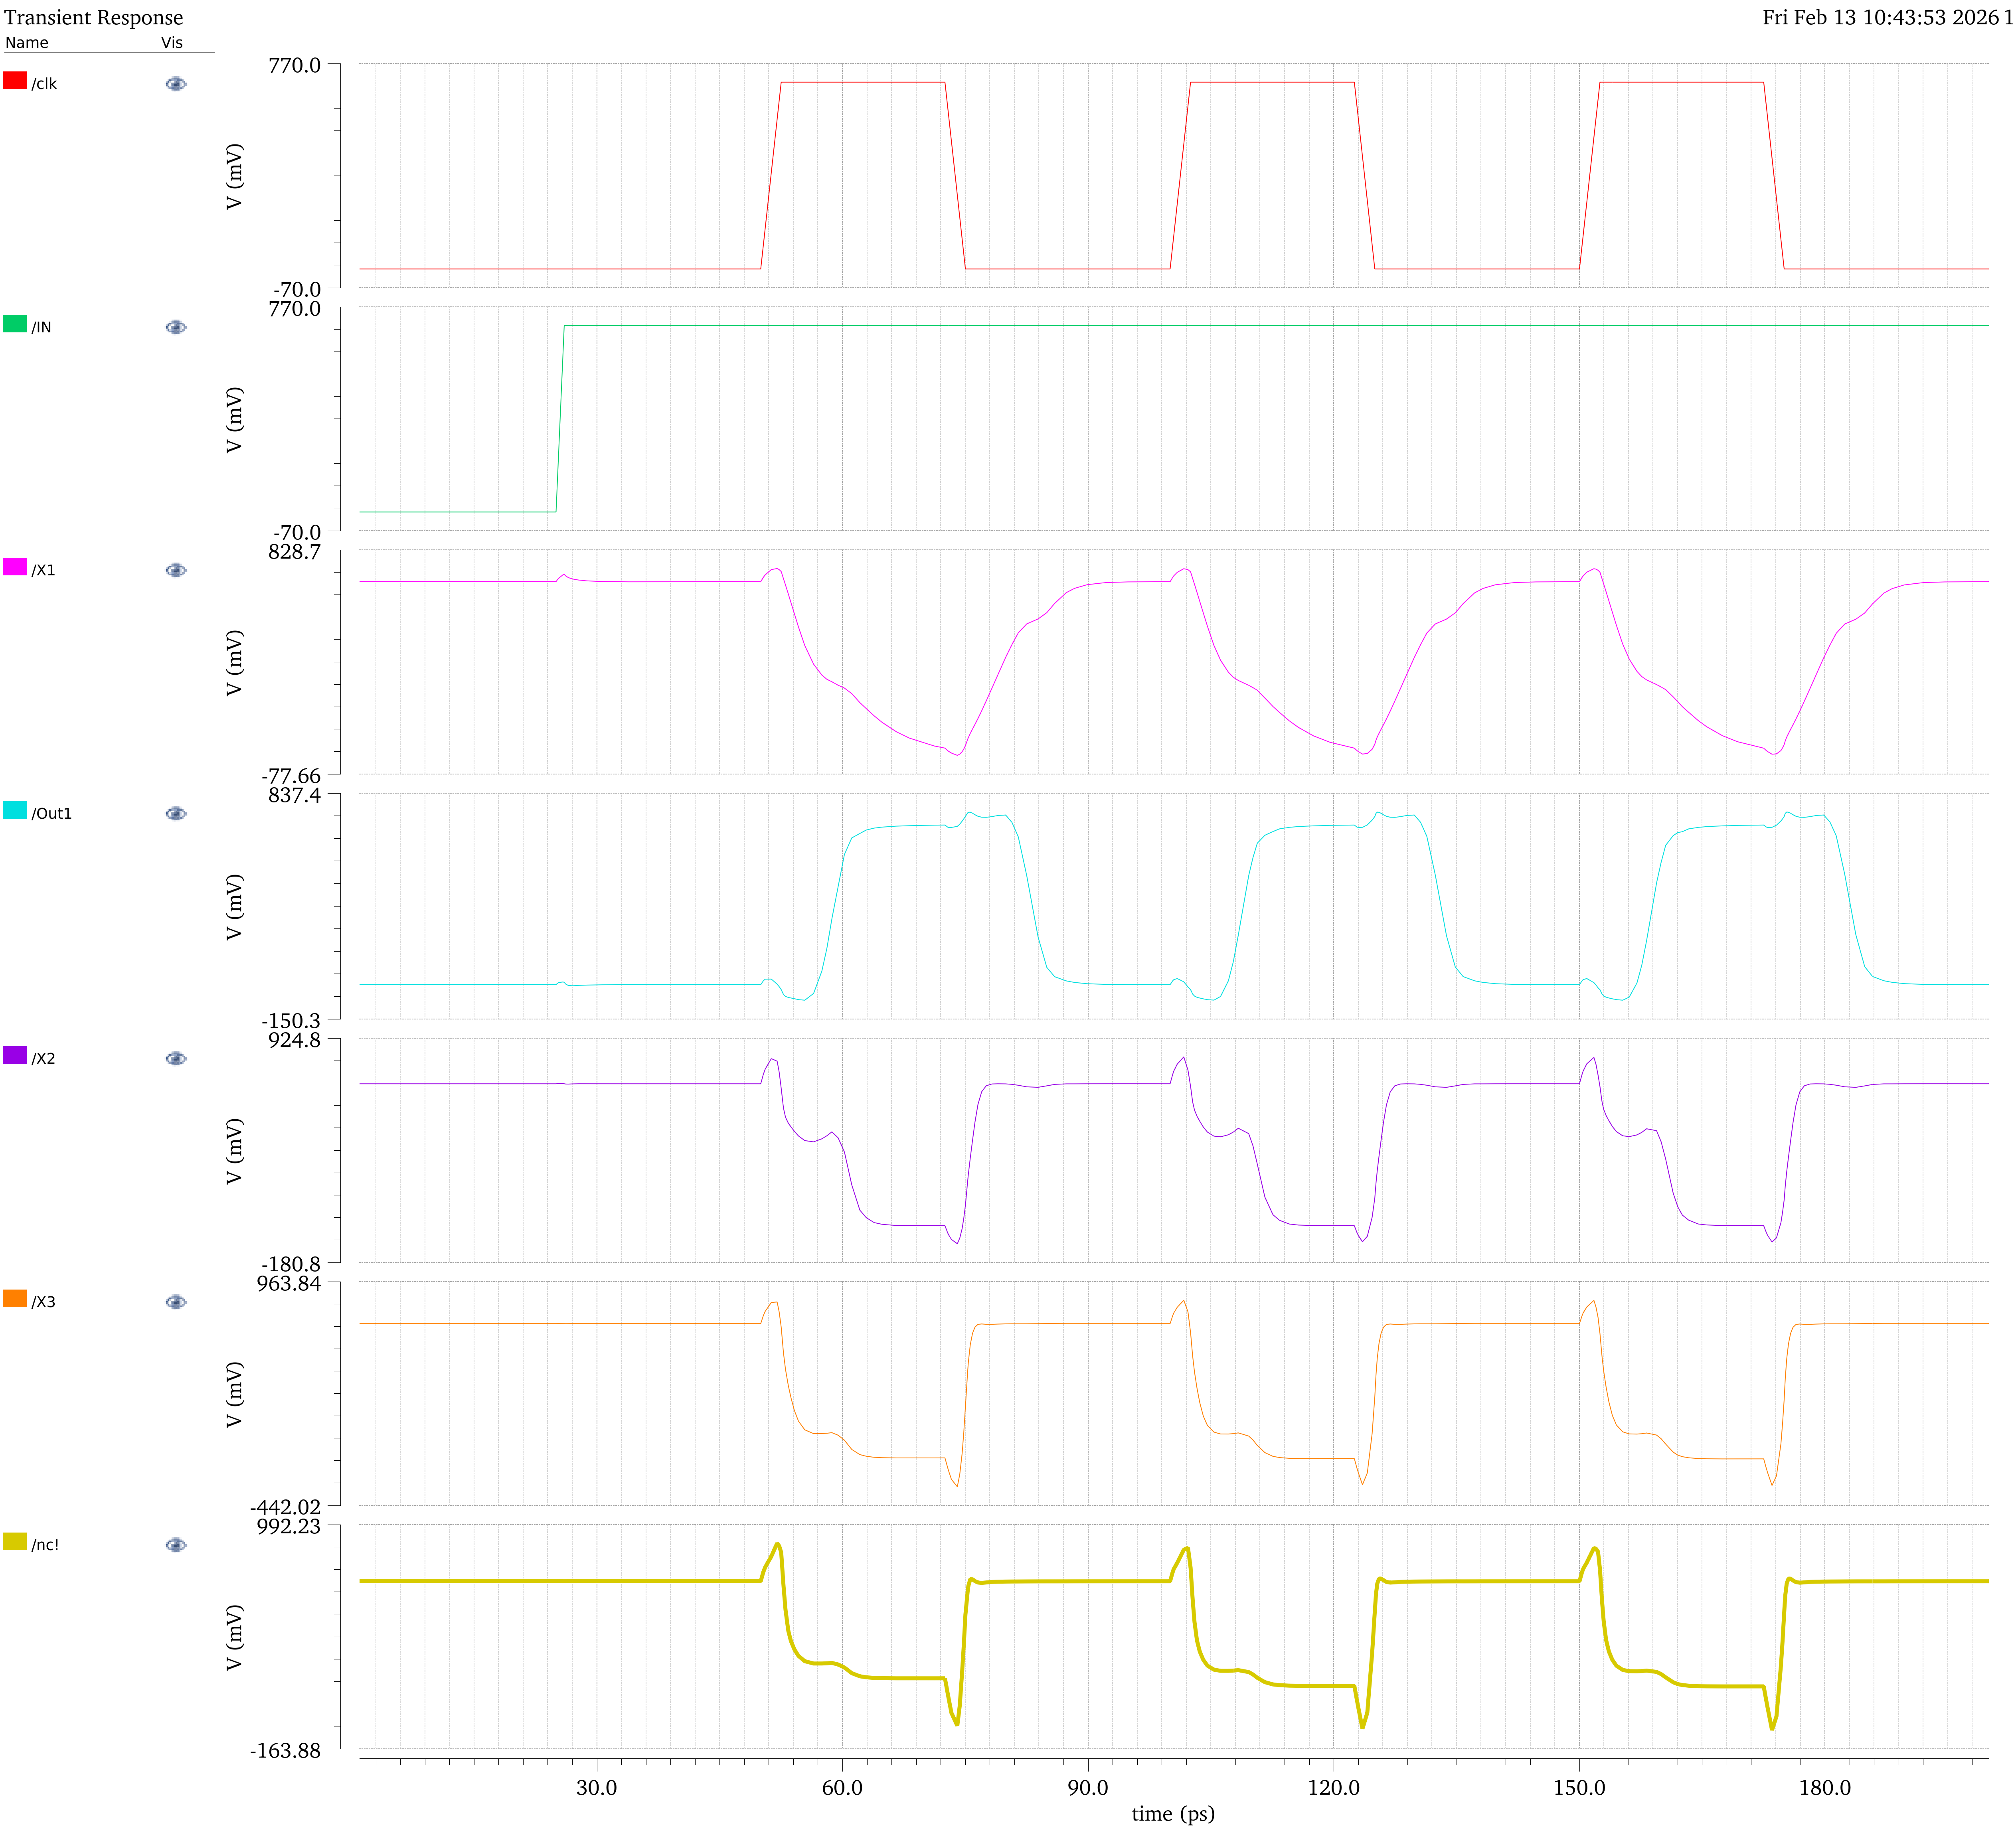
\includegraphics[width=0.49\linewidth, height=0.50\textheight, keepaspectratio]{Images/hw1_p4_vlsi_ii_2.png}\hfill
  \\[\smallskipamount]
  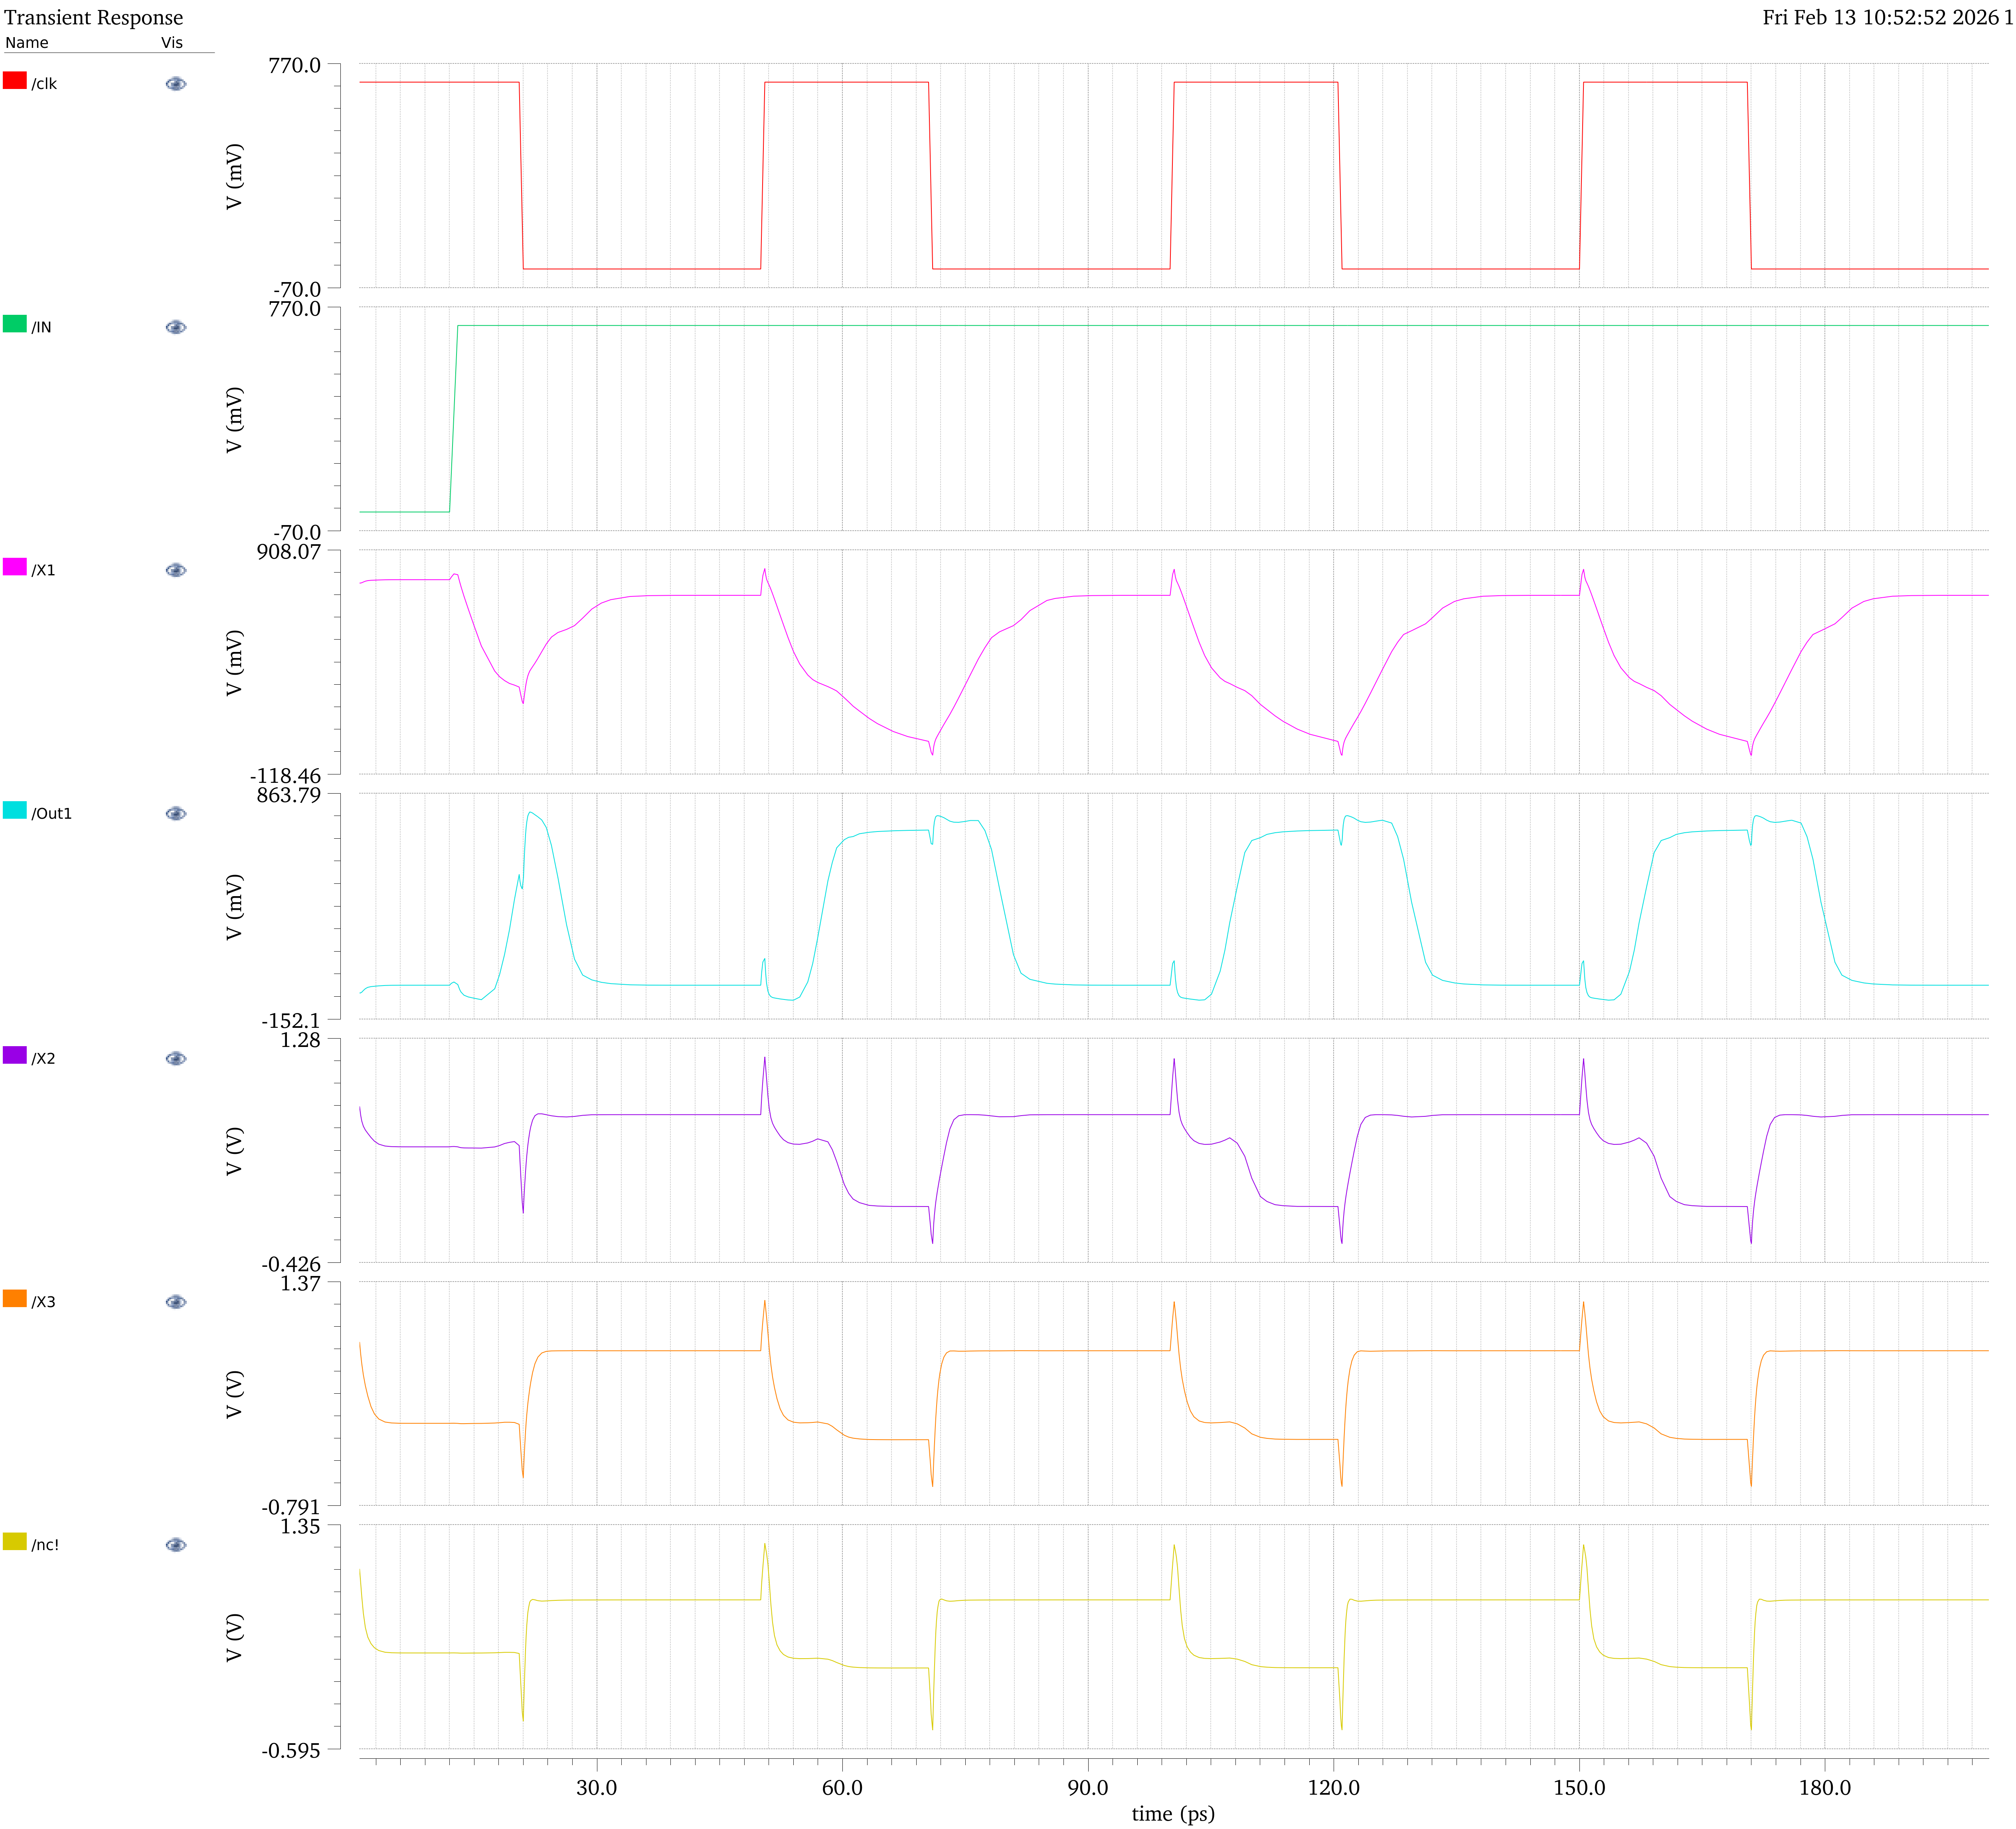
\includegraphics[width=0.79\linewidth, height=0.40\textheight, keepaspectratio]{Images/hw1_p4_vlsi_ii_3.png}\hfill
  \caption{Problem 4. Output a (left). Output b (middle). Output c (right).}
  \label{fid:output_p4}
  \parbox{\linewidth}{The circuit with the switches gives the incorrect logic response according to my sketches and simulations. The cirucits with no switches output the correct logic value. The difference from my sketches and 
  the simulation is due to the different delay period by the static inverters. And because of undervaluing the effect of voltage drops.}
\end{figure}

\end{document}

